% !TEX encoding   = UTF8
% !TEX spellcheck = ru_RU

\documentclass[a4paper,12pt,oneside,openany,final]{memoir}

% !TEX encoding   = UTF8
% !TEX spellcheck = en_US


%%% Page layout %%%
\usepackage{pdflscape}
\usepackage{geometry}

%%% Mathematics %%%
\usepackage{amsthm,amsfonts,amsmath,amscd}
\usepackage{mathtools}             % Add environment 'multlined'
\usepackage{dsfont}
\usepackage{unicode-math}

%%% Encodings and fonts %%%
\usepackage{polyglossia}[2014/05/21]  % Automatically load 'fontspec'

%%% Paragraph layout %%%
\usepackage{indentfirst}
\usepackage{epigraph}
\usepackage[style=french]{csquotes}

%%% Colors %%%
\usepackage[svgnames,table,hyperref]{xcolor} %,cmyk

%%% Tables %%%
\usepackage{longtable,ltcaption}
\usepackage{multirow,makecell}     % Advanced formatting
\usepackage{tabu,tabulary}         % Automatic columns width
\usepackage{array}
\usepackage{hhline}
\usepackage{multicol}

%%% General layout %%%
\usepackage{soulutf8}              % Underlying with hyphenation
\usepackage{icomma}
\usepackage{calc}
\usepackage[normalem]{ulem}

%%% Hyper references %%%
\usepackage{hyperref}

%%% Figures %%%
\usepackage[export]{adjustbox}
\usepackage{graphicx}
\usepackage{tikz}
\usetikzlibrary{arrows,decorations.pathmorphing,backgrounds,positioning,fit,calc}
\usetikzlibrary{arrows.meta}
\usetikzlibrary{shapes,shapes.misc}
\usetikzlibrary{graphs, graphdrawing}
\usegdlibrary{trees, layered}
\usepackage{wrapfig}

%%% Lists %%%
\usepackage[inline]{enumitem}

%%% Embedded languages %%%
\usepackage[usefamily={py,sympy},rerun=always]{pythontex}

%%% Listings %%%
\usepackage{verbatim}
\usepackage{minted}
\usepackage{listings}
\lccode`\~=0\relax                 % Fix \MakeLowercase etc. with (xe|lua)latex

%%% Smart references %%%
%\usepackage{cleveref}

%%% Style features %%%
\usepackage{lua-ul}

% !TEX encoding   = UTF8
% !TEX spellcheck = en_EN

\usepackage{csquotes}
\usepackage[backend=biber,%
            bibencoding=utf8,%
            citestyle=gost-inline-min,%gost-numeric,%
            bibstyle=gost-numeric,%
            sorting=none,%
            defernumbers=true,%
            sortcites=true,%
            doi=false,%
            isbn=false,%
            autolang=langname]{biblatex}


\DeclareFieldFormat{url}{
  \mkbibacro{URL}\addcolon\space\href{#1}{\nolinkurl{\thefield{urlraw}}}
}


% !TEX encoding   = UTF8
% !TEX spellcheck = en_US


%%% Hyper references colors %%%

\definecolor{linkcolor}{rgb}{0.9,0,0}
\definecolor{citecolor}{rgb}{0,0.6,0}
\definecolor{urlcolor}{rgb}{0,0,1}



%%% Define names %%%

\newcommand*\paperOrganization{\todo{Organization}}
\newcommand*\paperOrganizationShort{\todo{OShort}}
\newcommand*\paperDepartment{\todo{Department}}
\newcommand*\paperDepartmentShort{\todo{DShort}}
\newcommand*\paperTitle{\todo{Title}}
\newcommand*\paperSubject{\todo{Subject}}
\newcommand*\paperAuthor{\todo{\textcopyright{}perto}}
\newcommand*\paperKeywords{\todo{Keywords}}
\newcommand*\paperDate{\todo{Date}}
\newcommand*\paperYear{\todo{Year}}

% !TEX encoding   = UTF8
% !TEX spellcheck = en_US


%%% Redefine names %%%

\renewcommand*\paperOrganization{Московский физико-технический институт \\
    (государственный университет)}
\renewcommand*\paperOrganizationShort{МФТИ}
\renewcommand*\paperDepartment{Факультет аэромеханики и летательной техники}
\renewcommand*\paperDepartmentShort{ФАЛТ}
\renewcommand*\paperTitle{Программирование на языке \lang{C++}}
\renewcommand*\paperAuthor{\textcopyright Преподаватели}
\renewcommand*\paperKeywords{МФТИ, ФАЛТ, информатика, программирование, язык С++}
\renewcommand*\paperDate{\textit{2022--2023 уч.\,гг.}}
\renewcommand*\paperYear{2022--2023\,гг.}


\renewcommand*\paperSubject{\href{\latexurl}{\TeX}нические материалы семинаров}

% !TEX encoding   = UTF8
% !TEX spellcheck = en_US


%%% Template %%%

\DeclareRobustCommand{\todo}{\textcolor{red}}

\AtBeginDocument{%
  \setlength{\parindent}{2.5em}
}



%%% Encondings and fonts %%%

\setmainlanguage[babelshorthands=true]{russian}
\setotherlanguage{english}

\setmonofont{Source Code Pro}
\newfontfamily\cyrillicfonttt{Source Code Pro}

\defaultfontfeatures{Ligatures=TeX}  % NB! monofont settings should be before this

\setmainfont{STIX Two Text}
\newfontfamily\cyrillicfont{STIX Two Text}

\setsansfont{Source Sans 3}
\newfontfamily\cyrillicfontsf{Source Sans 3}

\setmathfont{STIX Two Math}
\newfontfamily\cyrillicfontmf{STIX Two Math}



%%% Captions %%%

\setlength{\abovecaptionskip}{0pt}
\setlength{\belowcaptionskip}{0pt}

\captionwidth{\linewidth}
\normalcaptionwidth



%%% Figures %%%

\setfloatadjustment{figure}{%
  \setlength{\abovecaptionskip}{0pt}
  \setlength{\belowcaptionskip}{0pt}
  \precaption{}
  \captionnamefont{\normalfont\normalsize}
  \captiondelim{~--- }
  \captionstyle[\centering]{\centering}
  \captiontitlefont{\normalfont\normalsize}
  \postcaption{}
}



%%% Subfigures captions %%%

\newsubfloat{figure}
\renewcommand{\thesubfigure}{\asbuk{subfigure}}
\subcaptionsize{\normalsize}
\subcaptionlabelfont{\normalfont}
\subcaptionfont{\!\!) \normalfont}  % round bracket after a letter
\subcaptionstyle{\centering}



%%% Tables %%%

\setfloatlocations{table}{!h}


%%% Hyper references settings %%%

\hypersetup{
  unicode,
  linktocpage=true,
%  linktoc=all,                % both the section and page part are links
%  pdfpagelabels=false,
  plainpages=false,
  colorlinks,
  linkcolor={linkcolor},
  citecolor={citecolor},
  urlcolor={urlcolor},
%  hidelinks,
  pdftitle={\paperTitle},
  pdfauthor={\paperAuthor},
  pdfsubject={\paperSubject},
  pdfkeywords={\paperKeywords},
  pdflang={ru},
}



%%% Lists %%%

\renewcommand{\labelitemi}{\normalfont\bfseries{--}}

%\renewcommand{\theenumi}{\alph{enumi}}
%\renewcommand{\labelenumi}{\theenumi)}

\makeatletter
\AddEnumerateCounter{\Asbuk}{\russian@Alph}{Щ}
\AddEnumerateCounter{\asbuk}{\russian@alph}{щ}
\makeatother

%\renewcommand{\theenumi}{\asbuk{enumi}}
%\renewcommand{\labelenumi}{\theenumi)}

\renewcommand{\theenumii}{\asbuk{enumii}}
\renewcommand{\labelenumii}{\theenumii)}

\renewcommand{\theenumiii}{\arabic{enumiii}}
\renewcommand{\labelenumiii}{\theenumiii)}

\setlist{%
  nosep,%
  labelindent=\parindent, leftmargin=*,%
  topsep=\medskipamount, itemsep=\smallskipamount%
}

\newlist{enumIssue}{enumerate}{1}
\setlist[enumIssue]{label=\Asbuk*., ref=\Asbuk*}

\newlist{enumissue}{enumerate}{1}
\newlist{enumissue*}{enumerate*}{1}
\setlist[enumissue,enumissue*]{label=\textit{\asbuk*}), ref=\textit{\asbuk*}}

\newlist{itemfeature}{itemize}{1}
\setlist[itemfeature]{label=--, topsep=\medskipamount}

\newlist{exercise}{enumerate}{1}
\setlist[exercise,1]{label={\arabic*.}, ref={\arabic*}, labelindent=0pt, widest={99}, itemsep=\bigskipamount, topsep=\bigskipamount}



%%% Listings %%%

\usemintedstyle{manni}

\renewcommand{\theFancyVerbLine}{%
  \textcolor{gray}{\tiny\arabic{FancyVerbLine}}%
}

\newmintinline{c}{fontsize=\small}
\newmintinline{cpp}{fontsize=\small}
\newmintinline{gas}{fontsize=\small}
\newmintinline{text}{fontsize=\small}

\newmint[cc]{c}{fontsize=\small, escapeinside=||}
\newmint{cpp}{fontsize=\small}
\newmint{js}{fontsize=\small}
\newmint{gas}{fontsize=\small}
\newmint[txt]{text}{fontsize=\small}
\newmint{console}{fontsize=\small}
\newmint[precomment]{text}{fontsize=\footnotesize, formatcom=\color{cyan}}

\newminted{c}{linenos, fontsize=\small, numbersep=0.2em, escapeinside=||}
\newminted{cpp}{linenos, fontsize=\small, numbersep=0.2em}
\newminted{gas}{linenos, fontsize=\small, numbersep=0.2em, tabsize=2}
\newminted{text}{fontsize=\small, tabsize=2}
\newminted{console}{fontsize=\small, tabsize=2}

\newmintedfile{c}{linenos, fontsize=\small, numbersep=0.2em}
\newmintedfile{cpp}{linenos, fontsize=\small, numbersep=0.2em}
\newmintedfile{js}{linenos, fontsize=\small, numbersep=0.2em}
\newmintedfile{gas}{linenos, fontsize=\small, numbersep=0.2em, tabsize=2}
\newmintedfile{objdump}{linenos, fontsize=\small, numbersep=0.2em, tabsize=2, escapeinside=||}
\newmintedfile{text}{fontsize=\small, tabsize=2}
\newmintedfile{console}{fontsize=\small, tabsize=2}


\newminted[precode]{text}{fontsize=\footnotesize, formatcom=\color{cyan}}



%%% General layout %%%

\DeclareRobustCommand*{\name}{\texttt}
\DeclareRobustCommand*{\code}[1]{\name{\small #1}}
\DeclareRobustCommand*{\codebf}[1]{\code{\bfseries #1}}
\DeclareRobustCommand*{\lang}[1]{\name{#1}}

\newcommand*{\comm}[1]{{\color{cyan}\ttfamily\footnotesize\itshape #1}}

\newcommand*{\styleans}[1]{\color{cyan}\underline{\color{gray}\ttfamily{}#1}}
\newcommand*{\showans}[1]{\phantom{#1}}
\newcommand*{\ansx}[1]{}
\newcommand*{\ansdots}[1]{\textcolor{cyan}{\ttfamily ...}}

\newcommand*{\ansfwnostar}[2]{\styleans{\makebox[#1][l]{\showans{#2}}}}
\newcommand*{\ansfwstar}[2]{\styleans{\makebox[#1][l]{\color{black}#2}}}
\newcommand*{\ansvwnostar}[1]{\styleans{\showans{#1}}}
\newcommand*{\ansvwstar}[1]{\styleans{\color{black}#1}}

\makeatletter
\newcommand*{\ansfw}{\@ifstar\ansfwstar\ansfwnostar}
\newcommand*{\ansvw}{\@ifstar\ansvwstar\ansvwnostar}
\makeatother

\newcommand*{\ArrowTo}[1]{%
  \tikz[baseline=#1]{
    \draw[white, -{Stealth[black, length=18pt, open]}] (0,0) -- (0.01,0)
  }%
}

\newcommand*{\mystyle}[1]{\textit{\ttfamily\footnotesize{}#1}}

% !TEX encoding   = UTF8
% !TEX spellcheck = en_US

%%% Figures %%%

\graphicspath{{images/}{../}{../../}}         % Пути к изображениям



%%% Page layout %%%

\geometry{a4paper,top=2cm,bottom=2cm,left=2.5cm,right=1cm} %,showframe,nofoot,nomarginpar
\setlength{\topskip}{0pt}
%\setlength{\footskip}{12.3pt} % to prevent warning



%%% Line spacing %%%

%\DoubleSpacing*
%\OnehalfSpacing*
%\setSpacing{1.42}   % like MS Word, may be include with previous line



%%% Align and hyphenation %%%

\tolerance 1414
\hbadness 1414
\emergencystretch 1.5em  % in case of problems the first parameter for tuning
\hfuzz 0.3pt
\vfuzz \hfuzz
%\raggedbottom
%\sloppy
\clubpenalty=10000
\widowpenalty=10000

\begin{russian}
  \hyphenation{не-пе-ре-се-каю-щих-ся}
\end{russian}


\setlength{\epigraphwidth}{0.3\textwidth}
\renewcommand{\epigraphsize}{\normalsize}
\epigraphrule = 0pt

\newfontfamily\epigraphfont[Scale=MatchLowercase]{TeX Gyre Chorus}



%%% Outline %%%

\renewcommand{\cftchapterdotsep}{\cftdotsep}

%\setrmarg{2.55em plus1fil}
\renewcommand{\cftchapterpagefont}{\normalfont}
\renewcommand{\cftchapterleader}{\cftdotfill{\cftchapterdotsep}}
%\renewcommand{\cftchapterfont}{}

\renewcommand\cftchapteraftersnum{.\space}
\renewcommand\cftsectionaftersnum{.\space}
\renewcommand\cftsubsectionaftersnum{.\space}
\renewcommand\cftsubsubsectionaftersnum{.\space}
\AtBeginDocument{%                                 % without this polyglossia make it
  \setsecnumformat{\csname the#1\endcsname.\space}
}

\renewcommand*{\cftappendixname}{\appendixname\space}



%%% Headlines %%%

\newcommand*{\headlinefont}{\normalfont\itshape\footnotesize\rmfamily}

\newcommand*{\footer}[1]{%
  \begin{tikzpicture}[baseline=\baselineskip,font=\headlinefont]
    \node[text=gray] {#1};
  \end{tikzpicture}%
}

\newcommand*{\footerleft}{\hspace{-1.5cm}\footer{\paperDepartmentShort{}, \paperOrganizationShort --- \paperTitle}}

\newcommand*{\footerright}{\footer{\paperAuthor, \paperYear}}

\makeoddhead{ruled}{\headlinefont \leftmark}{}{\headlinefont \rightmark}
\makeoddfoot{ruled}{\footerleft}{\thepage}{\footerright}
\makeoddfoot{plain}{\footerleft}{\thepage}{\footerright}
\pagestyle{ruled}



%%% Headings %%%

\chapterstyle{hangnum}

\settocdepth{subsection}


\newcommand*\AbstractSection[1]{%
  \section*{#1}
  \addcontentsline{toc}{section}{\numberline\ #1}
}

\newcommand*\WhatToReadSection{\AbstractSection{Что читать}}
\newcommand*\ExercisesSection{\AbstractSection{Упражнения}}
\newcommand*\TaskSection{\AbstractSection{Задание}}



%%% Counters %%%

\counterwithout{equation}{chapter}
\counterwithout{figure}{chapter}
\counterwithout{table}{chapter}



%%% Proper appendix numbering %%%

\makeatletter
\def\russian@Alph#1{\ifcase#1\or
   А\or Б\or В\or Г\or Д\or Е\or Ж\or
   И\or К\or Л\or М\or Н\or
   П\or Р\or С\or Т\or У\or Ф\or Х\or
   Ц\or Ш\or Щ\or Э\or Ю\or Я\else\xpg@ill@value{#1}{russian@Alph}\fi}
\def\russian@alph#1{\ifcase#1\or
   а\or б\or в\or г\or д\or е\or ж\or
   и\or к\or л\or м\or н\or
   п\or р\or с\or т\or у\or ф\or х\or
   ц\or ш\or щ\or э\or ю\or я\else\xpg@ill@value{#1}{russian@alph}\fi}
\makeatother



%%% Misc %%%

\newcommand*{\latexurl}{https://www.latex-project.org}
\newcommand*{\yadiskurl}{https://yadi.sk/d/XiUj9ZsNf3xHJ}
\newcommand*{\courseselfurl}{https://github.com/vpodaruev/programming-with-cpp}
\newcommand*{\mingwurl}{https://github.com/niXman/mingw-builds-binaries/releases/download/13.1.0-rt_v11-rev1/x86_64-13.1.0-release-posix-seh-ucrt-rt_v11-rev1.7z}
\newcommand*{\qtcreatorurl}{https://download.qt.io/official_releases/qtcreator/11.0/11.0.2/qt-creator-opensource-windows-x86_64-11.0.2.exe}
\newcommand*{\vscodeurl}{https://code.visualstudio.com/download}
\newcommand*{\giturl}{https://git-scm.com/downloads}
\newcommand*{\smartgiturl}{https://www.syntevo.com/smartgit/download}
\newcommand*{\smartgitacademicurl}{https://www.syntevo.com/register-non-commercial/\#academic}
\newcommand*{\sevenzipurl}{https://www.7-zip.org/download.html}
\newcommand*{\addtosyspathurl}{https://youtu.be/mQra00mT3Dg}
\newcommand*{\embedgitbashurl}{https://youtu.be/PzJCwfYfIzY?t=107}
\newcommand*{\typingtutorurl}{https://www.typingclub.com/sportal/program-3.game}
\newcommand*{\pythonurl}{https://www.python.org}
\newcommand*{\matplotliburl}{https://matplotlib.org}

\newcommand*{\yadisk}[1]{\name{\href{\yadiskurl}{яндекс-диск}/#1}}
\newcommand*{\GraphViz}{\href{http://www.graphviz.org}{\name{GraphViz}}}

\newcommand*{\GCC}{\textsf{\scshape gcc}}
\newcommand*{\GDB}{\textsf{\scshape gdb}}
\newcommand*{\git}{\texttt{\small Git}}

\newcommand*{\hard}{\makebox[0pt]{\hspace{-1.5\labelsep}\ensuremath{\mathsurround=0pt ^{\star}}}}
\newcommand*{\HardChapter}[1]{\chapter{\(^★\)#1}}
\newcommand*{\HardSection}[1]{\section{\(^★\)#1}}
\newcommand*{\HardSubsection}[1]{\subsection{\(^*\)#1}}

\newcommand*{\textbookref}[1]{\textit{#1}}



\addbibresource{references.bib}




\begin{document}

%%==========================
\begin{pycode}
from sympy import *
\end{pycode}
%%==========================


% !TEX encoding   = UTF8
% !TEX spellcheck = ru_RU

\thispagestyle{empty}%
\begin{center}%
  \paperOrganization
\end{center}%
%
\vspace{0pt plus 6fill}%
%
\begin{center}
  
\includegraphics[width=15em]{images/falt_logo.jpg}
\end{center}
%
\vspace{0pt plus 4fill}%
%
\begin{center}%
\paperDepartment
\end{center}%
%
\vspace{0pt plus 1fill}%
%
\begin{center}%
\textbf{\Huge\paperTitle}

\vspace{0pt plus 2fill}%
\textit{\large \paperSubject}

\vspace{0pt plus 4fill}%
\textcolor{violet}{\itshape\today}

\vspace{0pt plus 4fill}%
{Жуковский, \paperDate}
\end{center}


\frontmatter
%%==========
% !TEX encoding   = UTF8
% !TEX spellcheck = en_US

\clearpage

\ifdefmacro{\microtypesetup}{\microtypesetup{protrusion=false}}{}
\tableofcontents*
\ifdefmacro{\microtypesetup}{\microtypesetup{protrusion=true}}{}

% !TEX encoding   = UTF8
% !TEX spellcheck = ru_RU
% !TEX root = seminars.tex

%%================
\chapter{Введение}
%%================

%%=====================
\section{Цели и задачи}
%%=====================
\textit{Усвоить основы разработки, тестирования и отладки программ, базовые конструкции языка \lang{C++} и элементы стандартной библиотеки и получить практические навыки их использования при~решении ряда простых и более сложных задач.}

%%==========================
\paragraph{Структура курса.}
%%==========================
\begin{itemfeature}
  \item О курсе в~целом.
  \item Взаимосвязь с~другими курсами.

  \begin{flushleft}\hspace{-4em}\begin{tikzpicture}[node font=\small, >=Stealth]
    \graph [layered layout, components go right top aligned, layer sep=1em]
    {
      AppliedTasks/{Прикладные задачи} [blue, draw=blue, dashed, rounded corners] // [layered layout] {"Аэродинамика", "Динамика полёта", "Прочность", "Проектирование"};

      AppliedSoftware/{Прикладное программное обеспечение} [blue, draw=blue, dashed, rounded corners] // [layered layout, edge=white] {
        OpenFoam, SU2, Gmsh, FreeCAD, ParaView
      };

      OS/{Операционные системы} [blue, draw=blue, dashed, rounded corners, edge=black] // [tree layout] {
        Unix -> {
          Linux -> Android, FreeBSD -> {MacOS, iOS}, Solaris;
        },
        Windows
      };

      ComputerArchitecture/{Архитектура компьютера} [blue, draw=blue, dashed, rounded corners] // [layered layout, edge=<-] {
        "Архитектура и язык ассемблера"
        -> "Микроархитектура"
        -> "<<железо>>"
      };

      ComputerLanguages/{Языки программирования} [blue, draw=blue, dashed, rounded corners] // [layered layout, components go right top aligned, edge={<-, white}] {
        {Python, Java, PHP, HTML, Perl}
        -> {C++, Rust, ObjectiveC[as={Objective C}], Fortran}
        -> {C, Forth, Pascal}
      };

      Algorithms/{Алгоритмы и структуры данных} [blue, draw=blue, dashed, rounded corners] // [layered layout, edge=white] {
        {"Двоичный поиск", "Деревья"}
        -> {"Сортировка", "Хэш-таблицы"}
        -> {"Волновой алгоритм", "Графы"}
      };

      AppliedTasks ->[white] AppliedSoftware ->[white] {OS, ComputerLanguages} ->[white] {ComputerArchitecture, Algorithms};
    };
  \end{tikzpicture}\end{flushleft}

  \item Контрольно-проверочные мероприятия.
\end{itemfeature}



%%===========================
\section{Основная литература}
%%===========================
\cite{Stroustrup:2016:ru}

\nocite{Kernighan:2004:ru, Meyers:2006:ru, Meyers:2000:ru, Meyers:2002:ru, Meyers:2016:ru, Josuttis:2014:ru, Stroustrup:2006:ru, Stroustrup:2013:en}




%%===========================
\section{Материалы и задания}
%%===========================
Значительная часть обучающих упражнений и заданий содержится в~книге Бьярне Страуструпа. Дополнительные материалы размещены на~\href{\yadiskurl}{яндекс-диске\footnote{Материалы на Яндекс-диске: \nolinkurl{\yadiskurl}}}:
\begin{itemfeature}
  \item \codebf{books} "--- основная и дополнительная литература;
  \item \codebf{cpp-lectures} "--- лекционные материалы;
  \item \codebf{cpp-seminars} "--- семинарские материалы;
  \begin{itemize}
  	\item \codebf{/libs} "--- библиотеки, которые используются на занятиях;
  	\item \codebf{/program.pdf} "--- программа курса (темы для беседы на зачёте);
  	\item \codebf{/progress.pdf} "--- планы, успеваемость и проверочные мероприятия;
  	\item \codebf{/seminars.pdf} "--- вспомогательная методичка по материалам занятий.
  \end{itemize}
\end{itemfeature}

Исходный код примеров из данного учебного пособия доступен в \href{\courserepourl}{репозитории}\footnote{Репозиторий данного пособия: \nolinkurl{\courserepourl}} на~Git\,Hub, каталог \code{projects}.



%%===============================
\section{Программное обеспечение}
%%===============================
Интегрированная среда разработки (IDE "--- \textenglish{Integrated Development Environment}):
\begin{itemfeature}
  \item текстовый редактор,
  \item компилятор языка \lang{C++} (с~поддержкой стандарта \lang{C++14} или выше),
  \item редактор связей,
  \item средства сборки,
  \item средства отладки.
\end{itemfeature}



%%===========================================
\section{Установка и настройка рабочей среды}\label{sect:workEnv}
%%===========================================
Мы настоятельно рекомендуем в~качестве IDE установить \href{\vscodeurl}{\name{VS\,Code}}\footnote{\textenglish{Microsoft VS\,Code:} \nolinkurl{\vscodeurl}} от~Microsoft. Эта программа активно развивается, имеет полноценный современный редактор кода и поддерживает интеграцию со~множеством полезных инструментов (системой контроля версий, средствами форматирования кода, консолью). Распространяется свободно, кроссплатформенная, то есть доступна не~только под~Windows, но и под~Unix: GNU/Linux, Mac\,OS\,X. А также доступна на~территории России.

Запустите \name{VS\,Code}. Перейдите во вкладку <<Расширения>> на панели слева. Установите плагин \textenglish{C/C++ for Visual Studio Code}.

Далее необходимо установить \href{\smartgiturl}{\name{Smartgit}}\footnote{Syntevo Smartgit: \nolinkurl{\smartgiturl}} (или, в крайнем случае, просто \href{\giturl}{\git}\footnote{Система контроля версий Git: \nolinkurl{\giturl}}), оставляя рекомендуемые (по умолчанию) параметры в~тех местах, где вы сомневаетесь, что выбрать. \name{Smartgit} включает в себя дистрибутив \git-а, поэтому последний не нужно ставить отдельно.

\name{Smartgit} "--- это удобный и мощный графический пользовательский интерфейс, то есть окошки и кнопочки, для работы с~системой контроля версий \git. Это коммерческий продукт, однако, разработчик предоставляет некоммерческую лицензию для академических заведений, которую можно запросить, заполнив \href{\smartgitacademicurl}{форму}\footnote{Запрос лицензии: \nolinkurl{\smartgitacademicurl}} на сайте.

В~сочетании с дополнительными плагинами, \name{VS\,Code} частично предоставляет подобные возможности. Но, увы, это пока не так удобно.

Система контроля версий "--- неотъемлемый инструмент разработки сложных программ. Также он весьма полезен при~разработке небольших программ.



%%=====================
\paragraph{ОС Windows.}
%%=====================
Совместно с~\name{VS\,Code} используйте \href{\mingwurl}{\name{MinGW-w64}}\footnote{MinGW-w64: \nolinkurl{\mingwurl}} (компилятор, компоновщик, отладчик и прочее).

Для~этого:
\begin{itemfeature}
	\item \href{\sevenzipurl}{Распакуйте}\footnote{Архиватор 7-Zip: \nolinkurl{\sevenzipurl}} архив \name{MinGW-w64} в~каталог \code{c:\backslash{}mingw-64} или любой другой, куда вы обычно устанавливаете программы.

	\item \href{\addtosyspathurl}{Добавьте}\footnote{Adding Path to MinGW: \nolinkurl{\addtosyspathurl}} путь к~компилятору (\code{bin\backslash{}g++.exe}) в~список стандартных системных путей (системная переменная \name{PATH}).
\end{itemfeature}

Удобная Unix-подобная командная среда \name{Git\,Bash} идёт в~комплекте с~системой контроля версий \git{} (а также в~комплекте со~\name{Smartgit}-ом). Простые программы мы будем собирать непосредственно в~командной среде. Помимо прочего, она облегчит тестирование программ в~автоматическом и полуавтоматическом режимах.

\href{\embedgitbashurl}{Добавьте}\footnote{\textenglish{VS Code --- Integrate Git Bash as Default Terminal}: \nolinkurl{\embedgitbashurl}} \name{Git\,Bash} в~список доступных терминалов \name{VS\,Code} и выберите его в~качестве терминала по~умолчанию. (Файл с~именем \code{bash.exe} нужно найти в~каталоге установки \name{Smartgit}-а.)



%%==================
\paragraph{ОС Unix.}
%%==================
Пользователи Unix и подобных ей операционных систем могут установить средства сборки программ \name{GNU}/\GCC{} при~помощи менеджера системы управления пакетами (например, \code{apt} в~\name{Ubuntu} или \code{pamac} в~\name{Manjaro}). Командная среда \code{bash}, или подобная ей \code{zsh}, обычно доступна из~коробки и не~требует отдельной установки.



%%===================================
\paragraph{Если что-то пошло не так,}
%%===================================
повторите процедуру \textbf{спокойно}, выполняя \textbf{в~точности} все указанные выше действия. Попробуйте использовать только латиницу для~каталогов установки и проектов, иногда русские буквы в~путях или пробелы могут вызывать ошибки.



%%=================================
\paragraph{И теперь не получилось?}
%%=================================
Хм-м... Тогда обратитесь за~помощью к~товарищам в~группе, к~студентам старших курсов или, в~конце концов, к~преподавателю.



%%==================
\section{Что читать}
%%==================
\textcite{Stroustrup:2016:ru}: \textbf{главы~0, 1 и~2}



\mainmatter
%%=========
% !TEX encoding   = UTF8
% !TEX spellcheck = ru_RU
% !TEX root = ../seminars.tex

%%=====================
\chapter{Hello, World!}
%%=====================

%%==================================================
\section{Архитектура Фон-Неймана, уровни абстракции}
%%==================================================
Схематическое устройство компьютера. Алгоритмы и языки программирования. Абстракция от~реального <<железа>>.



%%=================
\section{Программы}
%%=================
\lang{С++}\footcite{Stroustrup:2019:ru} является компилируемым языком. Для работы программы её исходный текст должен быть обработан с~помощью компилятора, который создаёт объектные файлы, объединяемые компоновщиком в~выполнимую программу. Обычно программы на~языке \lang{С++} состоят из~многих файлов с~исходными текстами (именуемыми просто \textit{исходными файлами}).

\begin{center}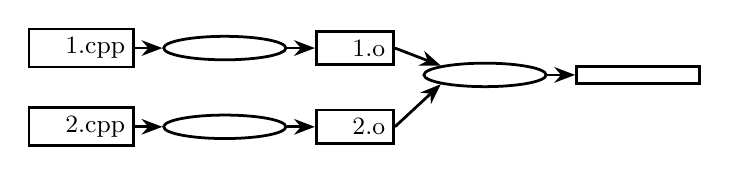
\begin{tikzpicture}[node font=\small, >=Stealth, line width=1pt]
    \graph [grow right sep, left anchor=east, right anchor=west, nodes=draw] {
    "файл1.cpp" -> c1/{компиляция} [ellipse] -> "файл1.o" ->[right anchor=north west] "компоновка" [ellipse, yshift=-2.5ex] -> "выполнимый файл"[yshift=-2.5ex];
    "файл2.cpp" -> c2/{компиляция} [ellipse] -> "файл2.o" ->[right anchor=south west] "компоновка";
    };
\end{tikzpicture}\end{center}

Выполнимая программа создаётся для~определённой комбинации аппаратного обеспечения и операционной системы; её нельзя просто перенести, скажем, из~компьютера Мac в~компьютер с~Windows. Говоря о~переносимости программ \lang{С++}, мы обычно имеем в~виду переносимость исходного кода, т.\,е. исходный код может быть успешно скомпилирован и выполняться в~разных
системах.

Стандарт ISO~\lang{С++} определяет два типа сущностей.
\begin{itemize}
\item \textit{Фундаментальные возможности языка}, такие как встроенные типы (например, \code{char} и \code{int}) или циклы (например, инструкции \code{for} и \code{while}).

\item \textit{Компоненты стандартных библиотек}, такие как контейнеры (например, \code{vector}, и \code{map}) или операции ввода--вывода (например, \code{<<} и \code{getline()}).
\end{itemize}

Компоненты стандартной библиотеки представляют собой совершенно обычный код \code{С++}, предоставляемый каждой реализацией языка. То есть стандартная библиотека \code{С++} может быть реализована в~самом \code{С++} (и реализуется "--- с~очень небольшим использованием машинного кода для~таких вещей, как переключение контекста потока). Это означает, что \code{С++} достаточно выразителен и эффективен для~самых сложных задач системного программирования.

\code{С++} является статически типизированным языком, т.е. тип каждой сущности (например, объекта, значения, имени или выражения) должен быть известен компилятору в~точке использования. Тип объекта определяет набор применимых к~нему операций.



%%===========================
\section{Структура каталогов}
%%===========================
Настоятельно рекомендуем упорядочивать файлы. Например, для семинарских программ и проектов можно использовать следующую структуру:
\begin{flushleft}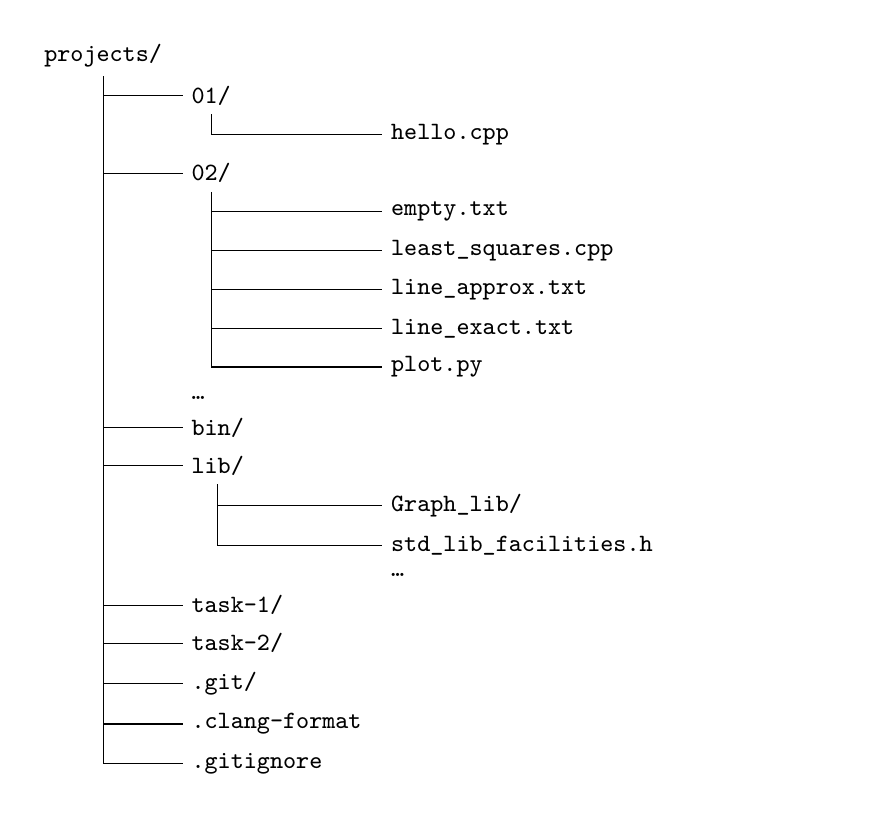
\begin{tikzpicture}[node font=\small\ttfamily]
		\matrix[row sep=0.2ex, column sep=0.5em]
		{
			\node (root) {projects/}; &  & &[-5em] \node[right] {\rmfamily все программы и проекты}; \\
			& \node[right] (sem1) {01/}; & & \node[right] {\rmfamily первое занятие}; \\
			& & \node[right] (hello) {hello.cpp}; & \\
			& \node[right] (sem2) {02/}; & & \node[right] {\rmfamily второе занятие}; \\
			& & \node[right] (test1) {empty.txt}; & \\
			& & \node[right] (lsm) {least\_squares.cpp}; & \\
			& & \node[right] (test2) {line\_approx.txt}; & \\
			& & \node[right] (test3) {line\_exact.txt}; & \\
			& & \node[right] (plot) {plot.py}; & \\
			& \node[right] {\ldots}; & & \\
			& \node[right] (bin) {bin/}; & & \node[right] {\rmfamily исполняемые файлы}; \\
			& \node[right] (lib) {lib/}; & & \node[right] {\rmfamily общие файлы и библиотеки}; \\
			& & \node[right] (graphlib) {Graph\_lib/}; & \\
			& & \node[right] (std) {std\_lib\_facilities.h}; & \\
			& & \node[right] {\ldots}; & \\
			& \node[right] (task1) {task-1/}; & & \\
			& \node[right] (task2) {task-2/}; & & \\
			& \node[right, text width=4em] (git) {.git/}; & & \node[right] {\rmfamily репозиторий системы контроля версий}; \\
			& \node[right] (format) {.clang-format}; & & \node[right] {\rmfamily стиль оформления кода}; \\
			& \node[right] (ignore) {.gitignore}; & & \node[right] {\rmfamily исключения для системы контроля версий}; \\
		};

		\draw (root) |- (sem1) (sem1) |- (hello);
		\draw (root) |- (sem2) (sem2) |- (test1)
		                       (sem2) |- (lsm)
		                       (sem2) |- (test2)
		                       (sem2) |- (test3)
		                       (sem2) |- (plot);
		\draw (root) |- (bin);
		\draw (root) |- (lib) (lib) |- (graphlib)
		                      (lib) |- (std);
		\draw (root) |- (task1);
		\draw (root) |- (task2);
		\draw (root) |- (git);
		\draw (root) |- (format);
		\draw (root) |- (ignore);
\end{tikzpicture}\end{flushleft}



%%=====================================
\section{Классическая первая программа}
%%=====================================
Наберите код классической первой программы (\code{hello.cpp}):

\cppfile{projects/01/hello.cpp}

Чтобы скомпилировать код, необходимо перейти (команда \code{cd}) в~каталог всех проектов:

\console'$ cd /path/to/your/projects'%$

\noindent и уже оттуда выполнить команду:

\console'$ g++ -Og -Wall -Wextra -pedantic -Ilib -o p 01/hello.cpp'%$

Здесь мы использовали следующие ключики (флаги) компилятора \code{g++}:
\begin{center}\begin{tabular}{lp{0.8\textwidth}}
    \toprule
    \code{-Og} & Задаёт разумный уровень оптимизации при~сохранении скорости компиляции и возможности отладки \\
    \code{-Wall} & Включает все предупреждения относительно конструкций, которые многие пользователи считают сомнительными и которые легко исправить \\
    \code{-Wextra} & Включает дополнительные предупреждения, которые не~включает \code{-Wall} \\
    \code{-pedantic} & Сообщает обо~всех нарушениях стандарта языка \lang{C++}. Отвергает программы, которые используют запрещённые расширения \\
    \code{-Ilib} & Добавляет каталог \code{lib} в~стандартные пути поиска компилятора. Таким образом, компилятор находит наш заголовок \code{std\_lib\_facilities.h} в~стандартных путях (когда, используя директиву \code{\#include}, мы указываем имя файла в~угловых скобках, а не в~двойных кавычках) \\
    \code{-o p} & Даёт исполняемому файлу имя \code{p}. В~\name{Windows} к~имени автоматически добавляется расширение \code{exe} \\
    \bottomrule
\end{tabular}\end{center}

Следом за~ключиками мы перечисляем все файлы с~исходным кодом (только \code{*.cpp} файлы). На первых порах у~нас будут программы, в которых весь код размещается в~одном файле. Немного позже мы начнём распределять код на~несколько модулей.

Если компиляция прошла успешно, то на~экране не~появится никаких сообщений. Можно вывести список файлов в~текущем каталоге, чтобы убедиться, что исполняемый файл с~именем \code{p} действительно появился.

\begin{consolecode}
$ ls
01  02  lib  p
\end{consolecode}

Теперь можно запустить программу на исполнение:
\begin{consolecode}
$ ./p
Hello, World!
\end{consolecode}

Текущий каталог (обозначается символом <<\code{.}>>) не~входит в~системные пути Unix, поэтому мы обязаны написать \code{./p}. Напротив, утилита \code{ls} расположена в~системных путях, поэтому не~требует уточнения пути.

В~дальнейшем рекомендуем сохранять бинарный (исполняемый) файл в~каталоге \code{bin}:
\begin{consolecode}
$ rm p
$ mkdir bin
$ ls
01  02  bin  lib
\end{consolecode}

\noindent Мы удалили (команда \code{rm}) файл~\code{p} и затем создали (команда \code{mkdir}) каталог \code{bin}.

\begin{consolecode}
$ g++ -Og -Wall -Wextra -pedantic -Ilib -o bin/p 01/hello.cpp
$ bin/p
Hello, World!
\end{consolecode}

\emph{Совет: чтобы избежать повторного набора команд в терминале, используйте стрелки~\code{\uparrow} и~\code{\downarrow} для~навигации по~истории команд.}



%%=============================
\section{Редактирование текста}
%%=============================
Набор исходного текста "--- неотъемлемая часть разработки программ. Используйте <<горячие>> клавиши для~более быстрого редактирования. Краткий список наиболее популярных комбинаций, поддерживаемых даже простыми редакторами:

{ % hot keys
\newcommand*{\hotkey}[1]{\fbox{\texttt{\small #1}}}
\newcommand*{\hotplus}{{\small\,+\,}}
\newcommand*{\hotkeys}[2]{\hotkey{#1}\hotplus\hotkey{#2}}
\newcommand*{\hotkeyss}[3]{\hotkey{#1}\hotplus\hotkey{#2}\hotplus\hotkey{#3}}

\begin{longtable}[l]{@{}rp{0.7\textwidth}@{}}
    \endhead
    \endfoot

    \hotkeys{Ctrl}{A} & Выделить всё \\[0.5em]

    \hotkeys{Ctrl}{C} & Скопировать выделение \\
    \hotkeys{Ctrl}{V} & Вставить \\[0.5em]

    \hotkeys{Ctrl}{Z} & Отменить последнее действие \\[0.5em]

    \hotkey{Home} & Переместить курсор в~начало\slash{}конец текущей строки \\
    \hotkey{End}  & \\[0.5em]

    \hotkeys{Shift}{Home} & Выделить символы с~текущей позиции и до~начала\slash{}конца строки \\
    \hotkeys{Shift}{End}  & \\[0.5em]

    \hotkeys{Ctrl}{Home} & Переместить курсор в~начало\slash{}конец файла \\
    \hotkeys{Ctrl}{End}  & \\
\end{longtable}

\noindent Дополнительные полезные комбинации в~\name{VS\,Code}:
\begin{longtable}[l]{@{}rp{0.7\textwidth}@{}}
    \endhead
    \endfoot

    \hotkeys{Ctrl}{\slash} & Комментировать\slash{}раскомментировать текущую строку или выделение \\[0.5em]

    \hotkeys{Alt}{\uparrow}   & Сместить текущую строку или выделение вверх\slash{}вниз \\
    \hotkeys{Alt}{\downarrow} & \\[0.5em]

    \hotkeyss{Alt}{Shift}{\uparrow}   & Дублировать текущую строку или выделение вверх\slash{}вниз \\
    \hotkeyss{Alt}{Shift}{\downarrow} & \\[0.5em]

    \hotkeyss{Ctrl}{Alt}{\uparrow}   & Редактировать столбец \\
    \hotkeyss{Ctrl}{Alt}{\downarrow} & \\
\end{longtable}
} % hot keys

Полезно научиться набирать текст вслепую, то есть не~глядя на~клавиатуру. В~сочетании с~использованием горячих клавиш, это позволяет достичь существенного ускорения при~наборе исходного кода. Таким образом, остаётся больше времени для~размышлений над~структурой и логикой самой программы. В~качестве примера он-лайн клавиатурного тренажёра приведём \href{\typingtutorurl}{эту}\footnote{Он-лайн клавиатурный тренажёр: \nolinkurl{\typingtutorurl}} ссылку.

Используйте моноширинный шрифт для~кода, например, \name{JetBrains\,Mono}. По~желанию, его можно \href{\jetbrainsfonturl}{скачать}\footnote{Шрифты JetBrains Mono: \nolinkurl{\jetbrainsfonturl}} и \href{\setupfonturl}{установить}\footnote{Как установить шрифт в~систему: \nolinkurl{\setupfonturl}} в~систему. Чтобы указать шрифт редактору, откройте файл с~настройками \name{VS\,Code} и добавьте такие строки:
\begin{minted}[fontsize=\small]{json}
    "editor.fontFamily": "JetBrains Mono",
    "editor.fontLigatures": false
\end{minted}
\noindent Если включить лигатуры, то некоторые составные операторы будут заменяться на более привычное начертание. Например, оператор \code{!=} будет выглядеть как \(\neq\).

Аккуратно оформляйте код, соблюдая правила хорошего \href{\codestyleurl}{стиля}\footnote{Стиль кода: \nolinkurl{\codestyleurl}}. Современные средства позволяют автоматически форматировать код согласно заданному стилю. Описание стиля \code{projects/.clang-format} есть в~\href{\courseselfurl}{репозитории}. В~настройки добавьте:

\begin{minted}[fontsize=\small]{json}
    "editor.formatOnSave": true
\end{minted}

Можно изменить стиль по вашему вкусу. Для этого отредактируйте загруженный файл, используя \href{\clangformatdocurl}{документацию}\footnote{Опции Clang-format: \nolinkurl{\clangformatdocurl}} утилиты \name{Clang-format}.



%%====================
\section{Unix утилиты}\label{sect:utils}
%%====================
Совместно с~командной средой \code{bash} (\textenglish{\textbf{b}ourne \textbf{a}gain \textbf{sh}ell}) поставляется широкий набор полезных программ, или утилит (\textenglish{utilities}).

\console/$ cd dir/%$

\textenglish{\textbf{c}hange \textbf{d}irectory} "--- перейти в~каталог \code{dir}. Если каталог опущен, то перейти в~домашний каталог. (Определяется значением переменной среды \code{HOME}.) Файловая система \textenglish{Unix} представляет собой единое дерево, и любой абсолютный путь начинается с~корня (\code{/}). Точка (\code{.}) означает текущий каталог, две точки (\code{..}) "--- родительский каталог.

\console/$ cd ../%$

Перейти в~родительский каталог.

\console|$ cd /|%$

Перейти в~корневой каталог.

\console/$ pwd/%$

\textenglish{\textbf{p}rint \textbf{w}orking \textbf{d}irectory} "--- вывести на~экран абсолютный путь к~текущему каталогу.

\console/$ ls dir/%$

\textenglish{\textbf{l}i\textbf{s}t} "--- вывести на~экран содержимое каталога \code{dir}. Если каталог опущен, то по~умолчанию используется текущий каталог.

\console/$ man cmd/%$

\textenglish{\textbf{man}ual} "--- вывести на~экран подробную справку о~команде \code{cmd}.

\console/$ cmd --help/%$

Вывести на~экран короткую справку о~команде \code{cmd}. Полезно, если утилита \code{man} недоступна.

\console/$ mkdir dir/%$

\textenglish{\textbf{m}a\textbf{k}e \textbf{dir}ectory} "--- создать каталог \code{dir}.

\console/$ rmdir dir/%$

\textenglish{\textbf{r}e\textbf{m}ove \textbf{dir}ectory} "--- удалить пустой каталог \code{dir}.

\console/$ rm file/%$

\textenglish{\textbf{r}e\textbf{m}ove} "--- удалить файл. Используя опцию \code{-r} можно рекурсивно удалить непустой каталог.

\console/$ mv src dst/%$

\textenglish{\textbf{m}o\textbf{v}e} "--- перемещает/переименовывает файл \code{src} в~\code{dst}. Имя \code{dst} может быть каталогом, тогда \code{mv} перемещает \code{src} туда.

\console/$ cat file.../%$

\textenglish{\textbf{cat}enate} "--- связывает файлы и выводит объединённое содержимое на~экран.

\console/$ less file/%$

Более мощный аналог утилиты \code{more} "--- постраничного фильтра для~просмотра файлов. Часто применяется для~буферизации вывода на~экран, используя конвейер:

\console/$ odjdump -d prog | less/%$


\console/$ vim file/%$

\textenglish{\textbf{v}isual editor \textbf{im}proved} "--- открыть файл для~редактирования. Пройти вводный курс по~использованию этого мощного редактора можно запустив команду:

\console/$ vimtutor/%$



%%==================================
\section{Интерпретатор \name{shell}}\label{sect:shell}
%%==================================
Когда система (в~терминале) выдаёт приглашение \code{\$} и вы вводите команды для~выполнения, вы имеете дело не с~ядром самой системы, а с~неким посредником, называемым интерпретатором команд, или \name{shell}\footnote{Более подробно об~интерпретаторе \name{shell} и других возможностях системы Unix излагается, например, в~книге \fullcite{Kernighan:1992:ru}}. Это обычная программа, но она может делать удивительные вещи. Применение программы--посредника обеспечивает три главных преимущества:

\begin{itemfeature}[itemsep=\baselineskip]
    \item Сокращённые имена файлов: можно задать целое множество файлов в~качестве аргументов команде, указав шаблон для имён: \name{shell} будет искать файлы, имена которых соответствуют заданному шаблону.

    \console/$ ls *.cpp *.c/%$

    Вывести на~печать имена всех файлов в~текущем каталоге, которые оканчиваются на~\code{.cpp} или \code{.c}. Символ \code{*} в~шаблоне соответствует любой последовательности символов. Поддерживаются и другие специальные символы для~задания шаблона.


    \item Переключение ввода--вывода: вывод любой программы можно направить в~файл, а не на~терминал, ввод можно получать из~файла, а не с~терминала. Ввод и вывод можно даже передать другим программам.

    \console/$ ls *.cpp > cppfiles.txt/%$

    Имена всех файлов, оканчивающихся на~\code{.cpp}, направить в~файл \code{cppfiles.txt}. Файл будет создан, если не~существует, или перезаписан, если существует.

    \console/$ wc -l < main.cpp/%$

    Подсчитать количество строк (опция \code{-l}) в~файле \code{main.cpp}.

    \console/$ cat main.cpp | wc -l/%$

    То же. Символ~\code{|} обозначает конвейер. Вывод команды слева передаётся на~ввод команде справа. Можно организовывать в~конвейере цепочку любой длины.

    \console/$ wc -l main.cpp/%$

    То же, используя лишь возможности самой утилиты \code{wc} (\textenglish{\textbf{w}ord \textbf{c}ount}).


    \item Создание собственной среды: можно определить свои собственные команды и правила сокращений.
\end{itemfeature}



%%============================================
\section{Система контроля версий \texttt{Git}}
%%============================================
Основы работы в~\git{} изложены в~книге \cite{Chacon:2023:ru}.

Это довольно обширный материал и представляет собой отдельный курс. Поэтому здесь мы рекомендуем прочитать главы <<Введение>> и <<Основы \git{}>> для первого знакомства с системой контроля версий.

Затем, полезно получить некоторой опыт работы с данной системой. И далее, перечитать эти главы, а также прочитать главу <<Ветвление в~\git{}>>. Этих возможностей вам будет вполне достаточно для успешного освоения данного курса.

Поняв суть и возможности системы контроля версий \git{}, очень просто освоить \name{Smartgit} "--- графическую обёртку. Каждая кнопка интерфейса выполняет в~консоли одну или несколько команд \git{}-а. Эти команды печатаются в~окне \textenglish{Output}. Попутно в~разных окнах отображаются состояние файлов, изменения от~версии к~версии, а также полное дерево истории коммитов. Встроенные средства позволяют не только сравнивать, принимать/отклонять, но и редактировать изменения.



%%================
\WhatToReadSection
%%================
\textcite{Stroustrup:2016:ru}: \textbf{глава~3} \\\indent
\textcite{Chacon:2023:ru}: \textbf{глава <<Основы \git{}>>}



%%===============
\ExercisesSection
%%===============
\begin{exercise}
\item Напишите программу, которая по заданному \(n\) находит \(n\)-е число Фибоначчи \(F_n\). Числа Фибоначчи определяются соотношениями:
\[
F_n = F_{n-1} + F_{n-2},\quad F_1 = F_2 = 1.
\]
Необходимо ли хранить в памяти все вычисленные числа Фибоначчи?

\item Напишите программу, которая принимает на входе число и печатает на экран его зеркальную копию, то есть, в <<перевёрнутом>> виде.

\item Напишите функцию, которая принимает на входе целое число и возвращает ответ, является ли оно простым. Протестируйте работу вашей функции.

\item Вычислите и сравните левую и правую части тождеств:
\begin{flushleft}
    \begin{enumerate*}[label=\arabic*), itemjoin={\qquad}]
        \item \(\sum\limits_{k=0}^{\infty}\dfrac{1}{(2k)!} = \dfrac{e + e^{-1}}{2}\);
        \item \(\prod\limits_{k=1}^{\infty} \dfrac{4k^2}{4k^2 - 1} = \dfrac{\pi}{2}\);
        \item \(e = \lim\limits_{n\to\infty} \dfrac{n}{\sqrt[n]{n!}}\);
    \end{enumerate*}
    \begin{flushright}
        \begin{enumerate*}[label=\arabic*), itemjoin={;\qquad}, resume]
            \item \(\dfrac{2}{1}\cdot
            \left( \dfrac{4}{3} \right)^{\frac{1}{2}}\cdot
            \left( \dfrac{6}{5}\dfrac{8}{7} \right)^{\frac{1}{4}}\cdot
            \left( \dfrac{10}{9}\dfrac{12}{11}\dfrac{14}{13}\dfrac{16}{15} \right)^{\frac{1}{8}}\cdot
            \ldots = e\).
        \end{enumerate*}
    \end{flushright}
\end{flushleft}
\end{exercise}
% !TEX encoding   = UTF8
% !TEX spellcheck = ru_RU
% !TEX root = ../seminars.tex

%%===========================
\chapter{Работа в \name{IDE}}\label{chap:ide}
%%===========================
В~ходе студенческой лабораторной работы по~физике получены данные измерений некоторой величины~\(y\), которая описывается линейной зависимостью \(y = a + bx\), где \(a\)~и \(b\) "--- какие-то константы. Полученные точки записаны в~файл, следуя простому формату:
\[
\begin{array}{ll}
    x_1 & y_1 \\
    x_2 & y_2 \\
    \vdots & \vdots \\
    x_N & y_N \\
\end{array}
\]
Количество пар координат не~указано и может быть произвольным. Несмотря на~линейную зависимость, точки не~ложатся строго на~прямую из-за различного рода погрешностей измерений.

Давайте напишем программу, которая считывает данные эксперимента из~файла и методом наименьших квадратов вычисляет коэффициенты \(a\) и \(b\), а также доверительные интервалы \(\pm\Delta a\) и \(\pm\Delta b\) соответственно.



%%==================================
\section{Метод наименьших квадратов}
%%==================================

%%===============================
\subparagraph{Постановка задачи.}
%%===============================
Рассмотрим регрессию (зависимость) следующего вида:
\begingroup
\newcommand{\SumN}{\ensuremath{\sum\limits_{i=1}^{N}}}
\[
y_i = a + b x_i + \varepsilon_i,\quad i = \overline{1, N}.
\]
Среди всевозможных значений \(\{ a, b \}\) будем искать такие, которые приводят к~минимальной сумме квадратов отклонений (ошибок):
\[
S_{\varepsilon} = \SumN \varepsilon_i^2 = \SumN (y_i - a - b x_i)^2\quad\rightarrow\quad \min\limits_{a, b}.
\]
Запишем условие существования экстремума:
\[
\begin{array}{l}
    \dfrac{\partial}{\partial a} S_{\varepsilon} = -2 \SumN (y_i - a - b x_i) = 0, \\[2ex]
    \dfrac{\partial}{\partial b} S_{\varepsilon} = -2 \SumN (y_i - a - b x_i) x_i = 0, \\
\end{array}
\]
откуда получим систему линейных уравнений:
\[
\left\{ \begin{array}{l}
    \SumN y_i - N a - b\SumN x_i = 0, \\[2ex]
    \SumN x_i y_i - a\SumN x_i - b\SumN x_i^2 = 0. \\
\end{array} \right.
\]
Вводя обозначение для среднего арифметического множества значений некоторой величины \(f\):
\[
\bar f = \dfrac{1}{N}\SumN f_i,
\]
перепишем систему в~виде:
\[
\left\{ \begin{array}{l}
    \bar y - a - b\bar x = 0, \\
    \overline{x y} - a\bar x - b\overline{x^2} = 0, \\
\end{array} \right.
\]
и получим искомое решение:
\[
\boxed{ \begin{array}{l}
        a = \bar y - b\bar x, \\
        b = \dfrac{\overline{x y} - \bar x\bar y}{\overline{x^2} - \bar x^2}. \\
\end{array} }
\]
\endgroup



%%====================================
\subparagraph{Программная реализация.}
%%====================================
Решение этой задачи может быть выражено на~языке \lang{C++} следующим образом:\label{code:lsm}

\cppfile{projects/02/least_squares.cpp}



%%====================
\subparagraph{Сборка.}
%%====================
Чтобы собрать исполняемый файл из командной среды, или <<консоли>>, необходимо перейти в каталог с вашими проектами:

\console`$ cd /path/to/your/projects`

\noindent и вызвать \GCC:

\console`$ g++ -o bin/lsm -std=c++17 -pedantic -Wall -Wextra 02/least_squares.cpp`

\begin{figure}[h]
{\centering
    \hfill
    \subbottom[точки лежат строго на прямой\label{fig:lsm:a}]{%
        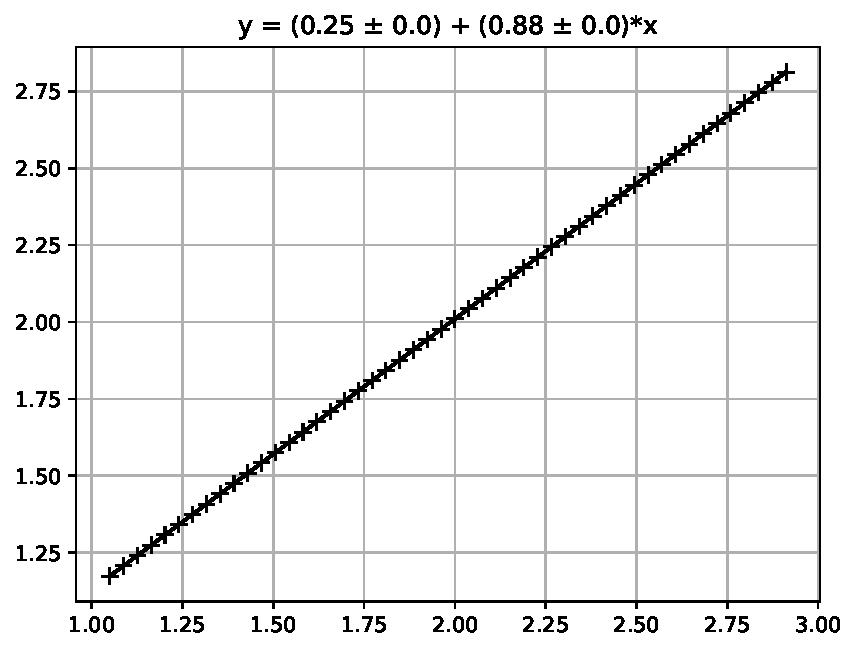
\includegraphics[width=0.45\textwidth]{images/line_exact.pdf}}
    \hfill
    \subbottom[точки не лежат на прямой\label{fig:lsm:b}]{%
        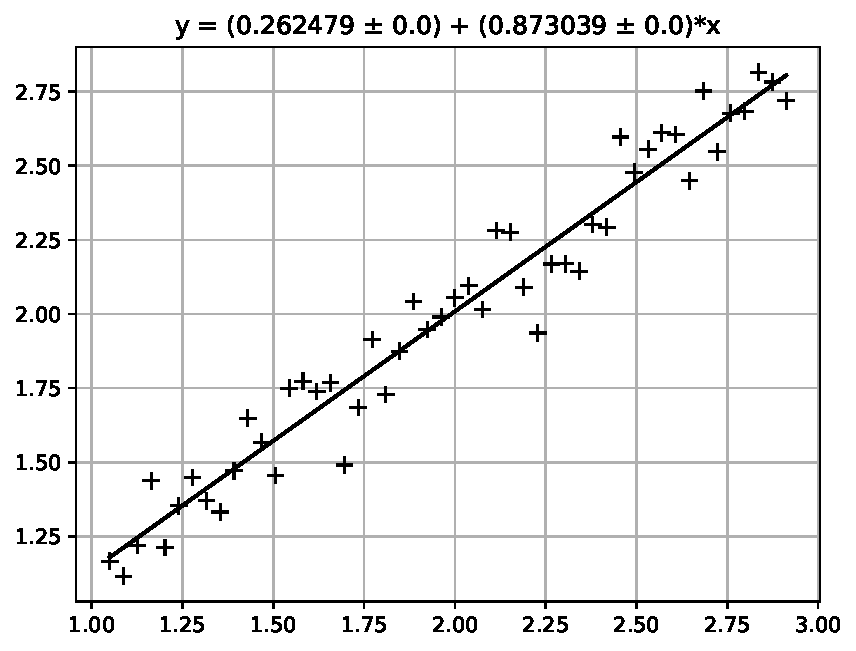
\includegraphics[width=0.45\textwidth]{images/line_approx.pdf}}
    \hfill
}
\caption{Линейная аппроксимация методом наименьших квадратов}
\label{fig:lsm}
\end{figure}



%%==========================
\subparagraph{Тестирование.}\label{test:lsm}
%%==========================
Полученная программа невелика, и, тем не менее, даже она может содержать приличное количество ошибок. Поэтому её работоспособность необходимо как следует проверить, запустив несколько разнообразных тестов. Приведём примеры:
\par\begin{itemfeature}
\item забыли указать имя файла:
\begin{consolecode}
$ bin/lsm
usage: bin/lsm  file_with_data
\end{consolecode}


\item файл не существует:
\begin{consolecode}
$ bin/lsm  not_exist.txt
error: can't open file 'not_exist.txt'
\end{consolecode}


\item файл пуст:
\begin{consolecode}
$ bin/lsm  02/empty.txt
error: division by zero
\end{consolecode}


\item идеальный случай (рис.\,\ref{fig:lsm:a}), когда точки лежат строго на прямой:
\begin{consolecode}
$ bin/lsm  02/line_exact.txt
line_exact.txt  0.25 0  0.88 0
\end{consolecode}


\item реальный случай (рис.\,\ref{fig:lsm:b}), когда точки лежат вдоль прямой с некоторым разбросом:
\begin{consolecode}
$ bin/lsm  02/line_approx.txt
line_approx.txt  0.262479 0  0.873039 0
\end{consolecode}
\end{itemfeature}



%%================
\WhatToReadSection
%%================
\textcite{Stroustrup:2016:ru}: \textbf{глава~4}



%%===============
\ExercisesSection
%%===============
\begin{exercise}
\item Доработайте программу, приведённую на странице~\pageref{code:lsm}. В функции \code{least\_squares} необходимо дополнительно вычислить доверительные интервалы.

Обязательно протестируйте вашу программу. Воспользуйтесь файлами, упомянутыми в подразделе на странице~\pageref{test:lsm}.


\item\hard\label{ex:plot} Продолжая предыдущее упражнение, напишите на \emph{любом} известном вам языке программу, которая рисует график, отражающий результаты лабораторной работы. На вход подаётся исходный файл с точками и оценки коэффициентов линейной регрессии.

Организуйте взаимодействие с программой из предыдущего упражнения так, чтобы можно было автоматически передавать входные данные. На выходе необходимо получить изображение на экране или в файле одного из популярных форматов, например \code{PNG}, с графиком, на котором маркерами нанесены экспериментальные точки, и сплошной линией "--- аппроксимирующая прямая.

Например, рисунок~\ref{fig:lsm} получен в результате выполнения этого упражнения с использованием языка \lang{Python}, пакета \name{Matplotlib} и командной среды (см. страницу~\pageref{sect:pyplot}).
\end{exercise}

% !TEX encoding   = UTF8
% !TEX spellcheck = ru_RU
% !TEX root = ../seminars.tex

%%==================
\chapter{Вычисления}
%%==================
Дополнительно к~материалу учебника рассмотрим несколько примеров простых вычислений. Для~расширения кругозора коротко покажем некоторые возможности открытой системы автоматической генерации документации из~комментариев в~коде \href{\doxygenurl}{\name{Doxygen}}\footnote{Документация по~Doxygen: \nolinkurl{\doxygenurl}}. Эта система работает с~кодом на~разных языках, не~только~\lang{C++}.

\begin{center}
  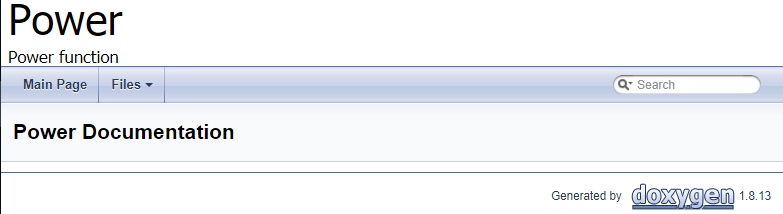
\includegraphics[width=0.75\textwidth]{images/doxygen_main_page.png}
\end{center}



%%================
\section{Рекурсия}
%%================
Рекурсия, или рекурсивный вызов, "--- это вызов функцией самой себя. Многие алгоритмы рекурсивны по~своей природе, и часто реализация с~использованием рекурсии оказывается проще, а также яснее выражает идею исходного варианта алгоритма.

\begin{center}
  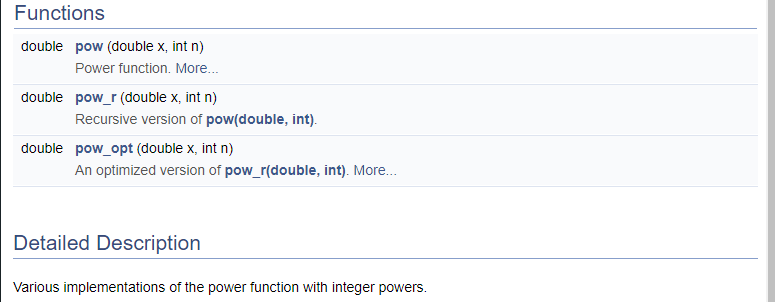
\includegraphics[width=0.75\textwidth]{images/doxygen_overview.png}
\end{center}

Рассмотрим функцию, вычисляющую значение \(x^n\). Вначале покажем итеративный вариант реализации, используя цикл:
\cppfile[firstline=6, lastline=21]{projects/03/power.cpp}

Обратите внимание на~оформление комментариев. Во-первых, к~привычным \code{//} добавлен ещё один \code{/}. Во-вторых, слова с~префиксом~@ являются командами \name{Doxygen}, при~помощи которых можно дать краткое описание функции, входных параметров, результата работы, а также подробно описать детали алгоритма, ограничения и прочее.

\begin{center}
  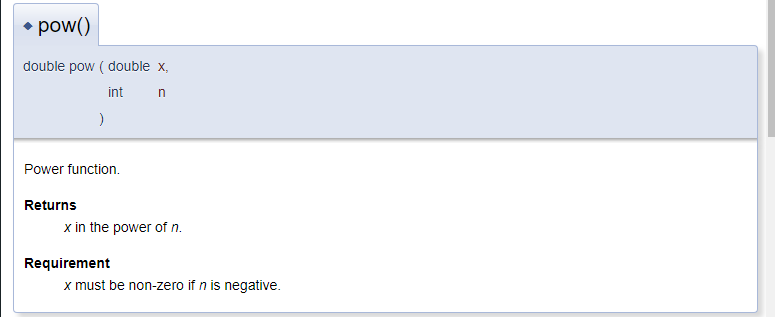
\includegraphics[width=0.75\textwidth]{images/doxygen_pow_description.png}
\end{center}

Теперь запишем рекурсивный вариант этой же функции:
\cppfile[firstline=24, lastline=33]{projects/03/power.cpp}

Алгоритм можно улучшить. Заметим, что для~чётных степеней \(n = 2k\) справедливо следующее соотношение:
\[
  x^n = x^{2k} = (x\cdot x)^k.
\]
А для~нечётных степеней \(n = 2k + 1\) будем действовать, как и раньше:
\cppfile[firstline=35, lastline=57]{projects/03/power.cpp}

В~комментариях можно разместить даже формулы в~стиле \href{\latexurl}{\LaTeX}-а. Также поддерживается упрощённое форматирование текста в~стиле \href{https://ru.wikipedia.org/wiki/Markdown}{\lang{Markdown}}.

\begin{center}
  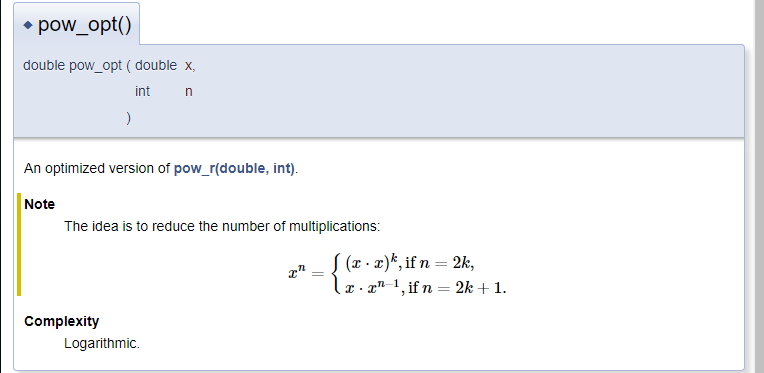
\includegraphics[width=0.75\textwidth]{images/doxygen_pow_opt_description.png}
\end{center}



%%==========================
\subparagraph{Тест-функция.}
%%==========================
Любой код, который написан нами, должен быть протестирован. Для~этой цели часто пишут вспомогательные функции. Например, в~нашем случае можно написать такой код:
\cppfile[firstline=59, lastline=89]{projects/03/power.cpp}

\noindent Строка:
\cppfile[firstline=69, lastline=69]{projects/03/power.cpp}

\noindent говорит, что имя \code{Func} "--- синоним типа, который указывает на~функцию с~двумя числовыми параметрами \code{double} и \code{int}, возвращающую число типа \code{double}.

Используя новый тип \code{Func} и макрос \code{FUN\_NAME}, мы создаём пары (указатель на~функцию, имя функции) и проходим по~каждой, вычисляя разницу с~эталонным значением функции \code{std::pow()} из~стандартной математической библиотеки.



%%=====================
\subparagraph{Макросы.}
%%=====================
Имя \code{FUN\_NAME} объявляется директивой \code{\#define} и является макросом, напоминая функцию тем, что имеет параметр. Директивы "--- инструкции, которые начинаются с~символа \code{\#}, "--- обрабатываются препроцессором перед компиляцией файла. Встречая макро-имя, препроцессор просто заменяет его на~тело в~макро-определении, подставляя параметры, если они есть.

\textbf{NB!} Не~используйте макросы без~крайней необходимости! Препроцессор действует весьма топорно. В~результате подстановки, код может привести к~неожиданному поведению. Рассмотрим простой пример:

\begin{cppcode*}{linenos=false}
#define N 10
#define M N + 5
// ...
int matrix_size = M * N;
\end{cppcode*}

\noindent Нетрудно догадаться, что в~результате макроподстановки мы получим количество элементов в~матрице \(10 + 5\cdot 10 = 60\), хотя изначально, скорее всего, планировали получить \((10 + 5)\cdot 10 = 150\). Зачастую, определения констант и многих макро-функций легко записать, используя \code{constexpr}-константы и \code{constexpr}-функции\footnote{Подробнее о~\texttt{constexpr}-функциях и их ограничениях можно прочитать в~книге \cite{Meyers:2016:ru, Stroustrup:2013:en}.}.
\enlargethispage{1\baselineskip}

\begin{cppcode*}{linenos=false}
constexpr int N = 10;
constexpr int M = N + 5;
\end{cppcode*}



%%========================
\subparagraph{Компиляция.}
%%========================
Чтобы собрать программу, необходимо добавить функцию \code{main()}:
\cppfile[firstline=91]{projects/03/power.cpp}

Для~компиляции вызовем следующую команду:

\console'$ g++ -Og -o bin/pow -Ilib -std=c++17 -pedantic -Wall -Wextra 03/power.cpp'



%%=========================
\section{Решето Эратосфена}
%%=========================
\emph{Решето Эратосф\'eна}\footcite{Eratosthen:wiki} "--- алгоритм нахождения всех простых чисел до~некоторого заданного целого числа~\(n\), который приписывают древнегреческому математику Эратосфену Киренскому. Название алгоритма говорит о~принципе его работы. Решето подразумевает фильтрацию, или отсеивание, всех чисел за~исключением простых. По~мере прохождения списка, нужные числа остаются, а ненужные (составные) исключаются.

Следуя методу Эратосфена, нужно выполнить следующие шаги:
\begin{enumerate}
    \item Выписать подряд все целые числа от~двух до~\(n\).
    \item Пусть переменная~\(p\) изначально равна двум "--- первому простому числу.
    \item\label{en:exclude} Зачеркнуть в~списке числа от~\(2p\) до~\(n\), считая шагами по~\(p\) (это будут числа кратные \(p\colon 2p, 3p, 4p,\ldots\)).
    \item\label{en:find} Найти первое незачёркнутое число в~списке, большее чем~\(p\), и присвоить значению переменной~\(p\) это число.
    \item Повторять шаги \ref{en:exclude} и \ref{en:find}, пока возможно.
\end{enumerate}
Теперь все незачёркнутые числа в~списке "--- это все простые числа от~\(2\) до~\(n\).

На~практике алгоритм можно улучшить. На~шаге \ref{en:exclude} числа следует зачёркивать, начиная сразу с~\(p^2\), потому что все составные числа меньше него уже будут зачёркнуты к~этому времени. И, соответственно, останавливать алгоритм можно, когда \(p^2\) станет больше, чем~\(n\). Также, все простые числа (кроме~\(2\)) "--- нечётные числа, и поэтому для~них можно считать шагами по~\(2p\), начиная с~\(p^2\).

Приведём возможный вариант реализации (см.~упражнение~13 из~\textbookref{главы~4} учебника):
\cppfile[firstline=11, lastline=37]{projects/03/eratosthen.cpp}

%%===================
\subparagraph{P.\,S.}
%%===================
\emph{Совет: не используйте для данной реализации \code{<std\_lib\_facilities.h>}.}

\noindent Помните, что каждую программу следует тщательно протестировать! Например, можно написать версию, использующую более простой алгоритм:
\cppfile[firstline=39, lastline=46]{projects/03/eratosthen.cpp}

\noindent И уже с~её помощью проверить, являются ли найденные числа простыми:
\cppfile[firstline=48]{projects/03/eratosthen.cpp}



%%================
\WhatToReadSection
%%================
\textcite{Stroustrup:2016:ru}: \textbf{глава~5}


%%===============
\ExercisesSection
%%===============
\begin{exercise}
\item Выполните упражнения из~\textbookref{главы~4} учебника.

\end{exercise}

% !TEX encoding   = UTF8
% !TEX spellcheck = ru_RU
% !TEX root = ../seminars.tex

%%==============
\chapter{Ошибки}
%%==============

%%==============================
\section{Игра <<Быки и Коровы>>}
%%==============================
Разберём вариант реализации игры <<Быки и Коровы>> (см.~упражнение~12 \textbookref{главы~5} учебника).
\cppfile[lastline=4]{projects/04/bulls_and_cows.cpp}

Начнём с~функции \code{main}. Обернём тело в~инструкцию \code{try-catch}, подразумевая обработку ошибок через механизм исключений:

\cppfile[firstline=45, lastline=47]{projects/04/bulls_and_cows.cpp}
\cpp'  // ...'
\cppfile[firstline=80]{projects/04/bulls_and_cows.cpp}

\noindent Фигурные скобки \code{main} опущены намеренно, поскольку тело будет заключено целиком внутрь блока \code{try}.

Размышляя об~игре, сформулируем для~начала правила и выведем на~экран подсказку для~пользователя нашей программки:

\cppfile[firstline=48, lastline=54]{projects/04/bulls_and_cows.cpp}

Укажем число, задуманное компьютером, непосредственно в~программе. Такое решение облегчит первоначальную отладку и сэкономит время разработки первой версии, откладывая размышления о~том, как задать число случайным образом да ещё так, чтобы цифры оказались уникальными. К~этому можно будет вернуться позднее.

Для~удобства доступа к~отдельным цифрам, поскольку их значения как целые числа нам не~нужны, будем хранить число в~виде последовательности символов.

\cppfile[firstline=56, lastline=56]{projects/04/bulls_and_cows.cpp}

Далее, следуя логике игры, пользователь должен попытаться угадать задуманное число. Необходимо дать ему возможность сделать ход и ввести данные. Этот код мы разместим, как отдельное логическое действие, в~функции \code{user\_guess}. А затем подсчитать количество <<быков>> и <<коров>> и вывести эту информацию на~экран:

\cppfile[firstline=58, lastline=77]{projects/04/bulls_and_cows.cpp}

Когда пользователь угадает число, то, очевидно, число <<быков>> станет равным количеству цифр в~задуманном числе, т.\,е. четырём. По~завершению цикла следует напечатать сообщение о~прекращении игры:

\cppfile[firstline=79, lastline=79]{projects/04/bulls_and_cows.cpp}

Теперь рассмотрим код для~вспомогательной функции \code{count}, которая подсчитывает количество цифр в~числе, совпадающих с~указанной.

\cppfile[firstline=6, lastline=15]{projects/04/bulls_and_cows.cpp}

Далее, напишем код, запрашивающий и получающий ввод от~пользователя:

\cppfile[firstline=29, lastline=43]{projects/04/bulls_and_cows.cpp}

Поскольку пользователь может ввести практически всё, что угодно, следует проверить входные данные на~соответствие правилам игры: должно быть четыре различные цифры:

\cppfile[firstline=17, lastline=27]{projects/04/bulls_and_cows.cpp}

Корректные входные данные позволяют нам не~предусматривать дополнительных проверок в~основном цикле функции \code{main}.



%%===================
\subparagraph{P.\,S.}
%%===================
Рассмотренный код "--- лишь основа для~создания хорошей игры. Вспомним хотя бы, что загадывание случайного числа мы отложили на~потом. Попробовав поиграть, становится очевидным, что необходимо вместо завершения программы после обработки исключения как-то возобновить игру. В~конце концов, пользователь мог случайно или по~ошибке нажать клавишу и ввести некорректный ответ. В~число улучшений самого кода следует включить устранение магической константы~4.

Продолжите работу над~игрой, выполняя упражнение~13 из~\textbookref{главы~5}.



%%================
\WhatToReadSection
%%================
\textcite{Stroustrup:2016:ru}: \textbf{глава~6}



%%===============
\ExercisesSection
%%===============
\begin{exercise}
\item Выполните упражнения из \textbookref{главы~5} учебника.
\end{exercise}

% !TEX encoding   = UTF8
% !TEX spellcheck = ru_RU
% !TEX root = ../seminars.tex

%%===========================
\chapter{Написание программы}
%%===========================

%%===================
\section{Калькулятор}
%%===================
Для~упражнений нам необходим код программы <<калькулятор>>, версия~2 из~\textbookref{главы~6}. Исходный файл загрузите из~репозитория
\begin{center}
  \courserepo{projects/05/calculator02buggy.cpp}.
\end{center}

Исправьте все ошибки (как ошибки компиляции, так и логические ошибки), которые специально внедрены в~эту версию кода.

Создайте файл \code{test\_in.txt}. Занесите туда все выражения, с~помощью которых вы тестировали работу вашей программы. Чуть позже мы покажем простой способ, как их подать на~вход программе непосредственно из~этого файла.

Используйте систему контроля версий (см.~раздел на~странице~\pageref{sect:git}) для~облегчения процесса разработки, ведения истории и создания разных ветвей кода, особенно, если они отличаются по~функциональным возможностям.



%%=====================================================
\section{Грамматика для побитовых логических выражений}
%%=====================================================
Побитовое логическое выражение напоминает арифметическое за~исключением того, что в~нём используются не~арифметические, а логические операторы: \cppinline{!}~(отрицание), \cppinline{~}~(дополнение), \cppinline{&}~(и), \cppinline{|}~(или) и \cppinline{^}~(исключающее или). Каждый оператор выполняет операции над~всеми битами своих целочисленных операндов. Операторы~\cppinline{!} и~\cppinline{~} являются префиксными унарными операторами. Оператор~\cppinline{^} имеет более высокий приоритет, чем оператор~\cppinline{|} (так же, как оператор~\cppinline{*} имеет более высокий приоритет, чем оператор~\cppinline{+}), так что выражение \cppinline{x|y^z} означает \cppinline{x|(y^z)}, а не~\cppinline{(x|y)^z}. Оператор~\cppinline{&} имеет более высокий приоритет, чем оператор~\cppinline{^}, так что выражение \cppinline{x^y&z} означает \cppinline{х^(y&z)}.

По~аналогии с~грамматикой обычных арифметических выражений, для логических побитовых выражений можно написать следующее:
\cppfile[firstline=14, lastline=29]{projects/05/bitwise_calculator.cpp}

Сделайте боковую ветку \code{bitwise-expr} в~системе контроля версий и переделайте код калькулятора так, чтобы он работал только с~целыми числами и вычислял значения побитовых логических выражений согласно разработанной грамматике.

Как убедиться, что ваша реализация работает правильно?



%%================
\WhatToReadSection
%%================
\textcite{Stroustrup:2016:ru}: \textbf{глава~7}



%%===============
\ExercisesSection
%%===============
\begin{exercise}
\item Выполните упражнения из~\textbookref{главы~6} учебника.
\end{exercise}

% !TEX encoding   = UTF8
% !TEX spellcheck = ru_RU
% !TEX root = ../seminars.tex

%%============================
\chapter{Завершение программы}\label{chap:completingprog}
%%============================

%%===================
\section{Калькулятор}
%%===================
Для~упражнений нам необходим код программы <<калькулятор>>, версия~8 из~\textbookref{главы~7}. Исходный файл загрузите из~репозитория
\begin{center}
    \courserepo{projects/06/calculator08buggy.cpp}.
\end{center}

Исправьте все ошибки (как ошибки компиляции, так и логические ошибки), которые специально внедрены в~эту версию кода.



%%==================================
\section{Автоматизация тестирования}
%%==================================
\enquote{При~приведении исходного текста в~порядок можно непреднамеренно внести новые ошибки. После наведения порядка в~исходном тексте всегда следует проводить повторное тестирование кода. Ещё лучше проводить его после внесения каждого улучшения, так что, если что-то пойдёт неправильно, вы всегда сможете вспомнить, что именно вы сделали только что. Помните: тестировать надо пораньше и почаще.}\footcite[глава~7, страница~282, последний абзац]{Stroustrup:2016:ru}

Также в~учебнике упоминается, и мы полностью с~этим согласны, что \enquote{тестировать вручную, постоянно вводя одни и те же выражения по~много раз, очень утомительно и требует времени. А всё, что утомительно, рано или поздно приводит к~ошибкам}. Так что давайте поскорее познакомимся, как можно автоматизировать этот процесс и облегчить себе жизнь.



%%========================================
\paragraph{Подготовка тестовых выражений.}
%%========================================
Поместите ряд примеров в~отдельный файл. Назовите его, допустим, \code{test\_in.txt}. Будьте изобретательны, составляя тестовые выражения. Стремитесь <<сломать>> программу. Можете обменяться исполняемыми файлами с~товарищем и найти примеры, на~которых его калькулятор выдаст ошибку в~правильном выражении, <<упадёт>> или даже зависнет. Используйте эти данные для~проверки своей программы. Вспомните примеры, на~которых ваш калькулятор уже <<ломался>> раньше. Добавьте эти выражения. Вспомните про~обработку ошибок. Специально вставьте несколько ошибочных выражений. Добавьте абракадабру. Калькулятор должен корректно и с~этим справляться, выдавая разумные сообщения об~ошибках. Итак, мы получим нечто такое:

\begin{textcode*}{linenos=false}
0; 1; 2; 3; 4; 5; 6; 7; 8; 9;

1 + 2;  1+2;  1 + 2 + 3;
1 - 2;  1-2;  1 - 2 - 3;

1 * 2;  1*2;  1 * 2 * 3;
1 / 2;  1/2;  1 / 2 / 3;

1 + 2*3;  1 - 2*3;
1 + 2/3;  1 - 2/3;

...

flkj430478908ufn5649058s6767-4
;
@$#!$%%^*()*()LKLKGJ58-099545567/*~~~~())(-=43+4;

...

let t;
let = 2;
let let = t;

let + x;

quit
\end{textcode*}

Подумайте хорошенько, все ли допустимые операции и возможности вы проверили? Добавьте лишние пробелы, переходы на~новую строку, табуляции. И, наоборот, в~некоторых примерах слепите всё вместе, убрав все пробельные символы. Будьте дотошны и упорны. Лучше отловить ошибки самому, чем досаждать ими пользователю! Подходите к~вопросу тестирования серьёзно и со~всей ответственностью.



%%=========================================
\paragraph{Перенаправление ввода и вывода.}\label{par:inout}
%%=========================================
Командный интерпретатор, или командная оболочка, доступен как в~\name{Unix}, включая \name{Linux} и \name{MacOS}, так и в~\name{Windows}. Родной интерпретатор \code{cmd} в~последней гораздо беднее по~возможностям в~сравнении с~\code{shell} в~\name{Unix}-подобных системах. Тем не~менее, вместе с~\git{} поставляется \code{GitBash} "--- вариант интерпретатора \code{shell}. Подробнее о~возможностях \code{shell} изложено в~разделе на~станице \pageref{sect:shell}.

Подадим полученные тестовые выражения из~файла на~стандартный поток ввода нашему калькулятору. Эти приёмы работают и в~\code{cmd}.

\console`$ bin/calc < 06/test_in.txt`

\noindent Сообщения программы на~экране также можно перенаправить из~стандартного потока вывода в~файл:

\console`$ bin/calc < 06/test_in.txt > 06/test_out.txt`

Заметим, что не~весь вывод с~экрана попал в~файл. Сообщения об~ошибках по-прежнему остались на~экране. Так произошло, потому что вывод ошибок производится в~поток \code{cerr}, а не~в~\code{cout}. Поток вывода ошибок (дескриптор 2) обычно отделён от~простого потока вывода (дескриптор 1). Тем не~менее, мы можем легко направить этот поток в~тот же файл, связав оба потока вместе:

\console`$ bin/calc < 06/test_in.txt > 06/test_out.txt 2>&1`



%%=================================
\paragraph{Автоматизация процесса.}
%%=================================
Убедившись, что корректные выражения приводят к~правильным ответам, а некорректные вызывают разумные сообщения об~ошибках, сохраните ответы под~другим именем.

\console`$ mv 06/test_out.txt 06/test_ans.txt`

Теперь с~лёгкостью можно получить вывод результатов работы программы после внесения каких-либо изменений: улучшений, исправлений "--- и протестировать все те возможности, что уже отлажены и должны работать.

Перекомпилируйте код после внесения очередных изменений.

\console`$ g++ -o bin/calc -Ilib -pedantic -Wall -Wextra 06/calculator.cpp`

Запустите программу и подайте ей тестовый ввод.

\console`$ bin/calc < 06/test_in.txt > 06/test_out.txt 2>&1`

Сравните результаты программно. Для этого, в~\name{Unix}, воспользуйтесь командой \code{diff}.

\begin{consolecode}
$ diff -s 06/test_out.txt 06/test_ans.txt
Files test_out.txt and test_ans.txt are identical
\end{consolecode}

\noindent Под~\name{Windows} существует более простая команда \code{fc}.

\begin{consolecode}
$ fc /l 06/test_out.txt 06/test_ans.txt
Сравнение файлов test_out.txt и TEST_ANS.TXT
FC: различия не найдены
\end{consolecode}

Если файлы отличаются, значит либо что-то перестало работать после изменений, либо же обнаружилась ошибка в~предыдущих результатах.



%%================
\paragraph{P.\,S.}
%%================
Сравнивать файлы можно любой программой с~графическим интерфейсом или без~него. Среди известных нам утилит отметим:

\begin{itemize}
\item \code{cmp} и \code{diff} "--- простые и надёжные консольные программы, способные <<переваривать>> файлы большого объёма, доступны в~\code{shell} и \code{GitBash};
\item \code{fc} "--- аналог \code{cmp}, но под~\name{Windows};
\item \code{meld} "--- с~графическим пользовательским интерфейсом, под~\name{Linux};
\item \code{WinMerge} "--- также с~графикой, но под~\name{Windows}.
\end{itemize}

\noindent Проверьте, возможно, ваша \name{IDE} уже включает в~себя подобные средства.

Если вы используете систему контроля версий, то добавив результаты--ответы под~контроль версий, легко сравнивать с~прежней версией средствами самой этой системы. Например, это легко делается в~уже упомянутом ранее \name{Smartgit}-е.



%%================
\WhatToReadSection
%%================
\textcite{Stroustrup:2016:ru}: \textbf{глава~8}



%%===============
\ExercisesSection
%%===============
\begin{exercise}
\item Выполните упражнения из~\textbookref{главы~7} учебника.

\end{exercise}

% !TEX encoding   = UTF8
% !TEX spellcheck = ru_RU
% !TEX root = ../seminars.tex

%%============================================
\chapter{Технические детали: функции и прочее}
%%============================================

%%=====================================
\section{Система сборки \texttt{CMake}}
%%=====================================
В~прошлый раз для~сборки исполняемого файла программы <<калькулятор>> мы вызывали следующую команду:

\console`$ g++ -o bin/calc -Ilib -pedantic -Wall -Wextra 06/calculator.cpp`

Для~проектов с~более сложной структурой, состоящих из~множества файлов, подключающих внешние библиотеки, имеющих разные варианты конфигурации сборки, намного удобнее воспользоваться системой сборки, например, простым \name{Make}-ом или более мощным и переносимым между платформами \name{CMake}-ом.

По~сути, для~системы сборки мы тоже некоторым образом должны указать детали всей цепочки сборки проекта от~компилятора и его флагов до~исходных файлов с~кодом.



%%===================================
\paragraph{Установка \texttt{CMake}.}
%%===================================
Скачайте \href{\cmakeurl}{архив}\footnote{Дистрибутив CMake: \nolinkurl{\cmakeurl}} \code{CMake} и распакуйте его (например, рядом с~каталогом, куда был распакован \code{MinGW}). Добавьте путь к~папке \code{bin} в~системные пути поиска (переменная \code{PATH}, см.~страницу~\pageref{sect:winSetup}).

Для~поддержки \name{CMake}-а в~\name{VS\,Code} необходимо доставить плагин \textenglish{VS Code Tools} от~Microsoft.

Поскольку данный плагин рассматривает рабочее пространство (\textenglish{workspace}) как один проект, то необходим общий проект, который будет включать в~себя дочерние проекты. Поэтому нам придётся создать проект с~нетривиальной структурой. К~счастью, это не~сильно усложнит нашу задачу.

Корневой и дочерние проекты \name{CMake} называются одинаково \code{CMakeLists.txt}, отличаясь лишь различным положением в~файловой системе.



%%======================
\paragraph{Общий проект}
%%======================
необходимо разместить в~корне рабочего пространства (у~нас это каталог \code{projects}). В~этот проект мы добавим общие настройки, такие как версия стандарта языка~\lang{C++} и дополнительные флаги компилятора (включим всевозможные предупреждения).

\cmakefile[firstline=3, lastline=5]{projects/CMakeLists.txt}

Далее, добавим в~стандартные пути каталог с~нашими библиотеками.

\cmakefile[firstline=7, lastline=11]{projects/CMakeLists.txt}

И, наконец, добавим наш первый дочерний проект, указав путь к~нему. (Создайте указанный каталог для~проекта.)

\cmakefile[firstline=13, lastline=13]{projects/CMakeLists.txt}



%%================================
\paragraph{Проект <<калькулятор>>}
%%================================
размещаем в~каталоге \code{projects/07/calculator}. Ещё раз повторим, что проектный файл создаётся один для~каждого каталога и поэтому на~всех уровнях вложения называется одинаково \code{CMakeLists.txt}. Эта идея наследуется от~\name{Make}.

Создадим локальную переменную \code{TARGET}. Она будет использоваться несколько раз. Будет удобно копировать проект для~других задач и заменять имя проекта только один раз в~этом месте.

\cmakefile[firstline=3, lastline=3]{projects/07/calculator/CMakeLists.txt}

Укажем имя проекта и язык программы. Для получения значения локальной переменной используется синтаксис \code{\$\{TARGET\}}.

\cmakefile[firstline=5, lastline=5]{projects/07/calculator/CMakeLists.txt}

Сообщим системе сборки, что нам нужен исполняемый файл и что исходный код расположен в~одном файле. (Если файлов несколько, просто перечисляем их через пробел или с~новой строки.)

\cmakefile[firstline=7, lastline=10]{projects/07/calculator/CMakeLists.txt}

В~завершение попросим систему сгенерировать инструкции для~установки целевого файла в~заданный каталог. Для~упрощения понимания, можно считать, что файл будет просто скопирован\footnote{В~реальности могут выполняться дополнительные действия в~зависимости от~целевого файла и целевой платформы.}.

\cmakefile[firstline=12, lastline=12]{projects/07/calculator/CMakeLists.txt}



%%==========================================
\paragraph{Как назначить каталог установки?}
%%==========================================
В~настройки рабочего пространства (\textenglish{Workspace Settings JSON}) необходимо добавить строку:

\jsonfile[firstline=5, lastline=5]{projects/.vscode/settings.json}

Чтобы выполнить установку, необходимо явно вызвать команду: \code{Ctrl+Shift+P} и в~строке поиска набрать \code{cmake\,install}.

Таким образом, исполняемый файл окажется в~каталоге \code{projects/bin}, как и ранее, когда мы непосредственно вызывали компилятор из~консоли.



%%================
\paragraph{P.\,S.}
%%================
Поиск компилятора, настройку флагов компиляции и массу другой работы \code{CMake} выполнит вместо нас в~процессе конфигурации. Этим процессом можно управлять. Однако, в~данный момент, нас вполне устроят базовые пресеты (\textenglish{Release, Debug}). Подробнее про систему сборки \code{CMake} можно почитать в~\href{\cmakedocurl}{документации}\footnote{Документация CMake: \nolinkurl{\cmakedocurl}}.



%%====================================
\section{Распределение кода по файлам}
%%====================================
Разместите логически отдельные части калькулятора в~разных файлах, опираясь на~материал \textbookref{главы~8}.

\begin{flushleft}\begin{tabular}{ll}
    \toprule
    \code{token.h}   & Лексемы и поток ввода лексем, константы \\
    \code{token.cpp} & \\[0.5em]

    \code{variable.h}   & Переменные и таблица переменных (символов) \\
    \code{variable.cpp} & \\[0.5em]

    \code{calculator.cpp} & Цикл вычислений, реализация грамматики \\
    \bottomrule
\end{tabular}\end{flushleft}

Помните, что заголовочные файлы должны содержать лишь объявления и константы, чтобы при~включении в~другие единицы трансляции не~происходило переопределение функций и глобальных переменных.

Как правило, содержимое заголовочного файла обрамляется директивами:

\begin{cppcode*}{linenos=false}
#ifndef TOKEN_H
#define TOKEN_H 1

// all code must be here

#endif // #ifndef TOKEN_H
\end{cppcode*}

\noindent Это необходимо во~избежание повторного включения кода из~файла \code{token.h} в~ту же единицу трансляции. (Когда и к~чему это может привести?) Такая ситуация неизбежно возникает в~любой достаточно большой программе.

Директива \cppinline/#ifndef/ проверяет определено ли имя \cppinline/TOKEN_H/. Если да, то она игнорирует весь код вплоть до~завершающей парной директивы \cppinline/#endif/. Если нет, тогда код включается, а \cppinline/TOKEN_H/ определяется при~помощи \cppinline/#define/, чтобы при~повторном подключении файла этот код пропускался. Имя макроса обычно формируют по~названию исходного заголовочного файла и набирают в~верхнем регистре.

Приведённый выше способ является наиболее переносимым между различными платформами. Некоторые компиляторы дополнительно поддерживают директиву, которая, по~сути, служит той же цели:

\cpp/#pragma once/



%%===========================
\section{Замена потока ввода}
%%===========================
Сделайте поток лексем явным параметром функций, как требуется в~упражнении~1 из~\textbookref{главы~8}. Например, функция \code{statement()} будет выглядеть так:

\begin{cppcode*}{linenos=false}
double statement (Token_stream& ts)
{
  Token t = ts.get();
  switch (t.kind)
  {
    case let:
      return declaration(ts);
    default:
      ts.putback(t);
      return expression(ts);
  }
}
\end{cppcode*}

\noindent Глобальную переменную \code{ts} можно (и нужно) сделать локальной:
\begin{cppcode*}{linenos=false}
void calculate ()
{
  Token_stream ts;

  while (true)
  try
  {
// as before

    out << result << statement(ts) << endl;
  }
  catch (runtime_error& e)
  {
// ...
    clean_up_mess(ts);
  }
}
\end{cppcode*}

\noindent Добавьте в~класс \code{Token\_stream} ссылку на~поток ввода и соответствующий конструктор для~инициализации. По~умолчанию, как и ранее, используйте стандартный поток ввода \code{cin}:

\begin{cppcode*}{linenos=false}
class Token_stream
{
  public:
  Token_stream() : in{ cin } {/* empty body */}
  Token_stream(istream& s) : in{ s } {/* empty body */}

// as before

  private:
// ...
  istream& in;
};
\end{cppcode*}

\noindent Определения методов класса следует поправить, заменив \code{cin} на~\code{in} иное подходящее имя.



%%================
\paragraph{P.\,S.}
%%================
После всех изменений, необходимо вновь прогнать тесты (см.~раздел на~странице~\pageref{sect:autotests}) и убедиться, что калькулятор остался в~рабочем состоянии.



%%==================================
\section{\texttt{constexpr} функции}
%%==================================
Немного дополним материл \textbookref{главы~8} по~данной теме\footcite[раздел 3.9]{Meyers:2016:ru}.

\begin{itemize}[itemindent=*, leftmargin=0pt]
    \item Функции, объявленные как \cppinline/constexpr/, могут использоваться в~контекстах, требующих константы времени компиляции. Если значения передаваемых вами аргументов в~\code{соnstехрr}-функцию в~таком контексте известны во~время компиляции, результат функции будет вычислен в~процессе компиляции. Если любое из~значений аргументов неизвестно во~время компиляции, ваш код будет отвергнут.

    \item Когда \code{соnstехрr}-функция вызывается с~одним или несколькими значениями, неизвестными во~время компиляции, она действует так же, как и обычная функция, выполняя вычисления во~время выполнения. Это означает, что вам не~нужны две функции для~выполнения одних и тех же операций, одной "--- для~констант времени компиляции, другой "--- для~всех прочих значений. Функция, объявленная как
    \code{constexpr}, выполняет их все.
\end{itemize}

Поскольку функции \code{constexpr} должны быть способны возвращать результаты во~время компиляции при~вызове со~значениями времени компиляции, на~их реализации накладываются ограничения. Эти ограничения различны в~\lang{C++11} и~\lang{C++14}.

В~\lang{C++11} функции \code{constexpr} могут содержать не~более одной выполнимой инструкции "--- \cppinline/return/. Это выглядит более ограничивающим, чем является на~самом деле, поскольку для~повышения выразительности \code{соnstехрr}-функций можно использовать две хитрости. Во-первых, можно применять условный оператор \code{"? :"} вместо инструкции \cppinline/if-else/, а во-вторых, вместо циклов можно использовать рекурсию. Таким образом, функция \code{pow} может быть реализована следующим образом:

\begin{cppcode*}{linenos=false}
constexpr int pow (int base, int exp) noexcept
{
  return exp == 0 ? 1 : base * pow(base, exp - 1);
}
\end{cppcode*}

Этот код работает, но только очень непритязательный функциональный программист сможет назвать его красивым. В~\lang{C++14} ограничения на~\code{constexpr}-функции существенно слабее, так что становится возможной следующая реализация:

\begin{cppcode*}{linenos=false}
constexpr int pow (int base, int exp) noexcept  // C++14
{
  auto res = 1;
  for (int i = 0; i < exp; ++i)
    res *= base;
  return res;
}
\end{cppcode*}



%%=====================================
\section{Сортировка пар (имя, возраст)}
%%=====================================
Приведём пример реализации программы из~упражнения~7 \textbookref{главы~8}. Будем придерживаться контекста исходного задания из~книги и использовать лишь изученные нами средства.

В~начале мы должны отсортировать вектор имён, а затем синхронизировать его с~вектором возрастов, используя копии исходных массивов.

\cppfile[firstline=48, lastline=56]{projects/07/name_age.cpp}

Чтобы синхронизировать пары, будем брать имена из~нового, сортированного, массива и искать их позицию в~старом массиве-копии. Взяв элемент из~старого массива возрастов с~той же позицией, мы получим парный элемент для~текущего имени.

\cppfile[firstline=28, lastline=46]{projects/07/name_age.cpp}

\noindent Отметим, что в~исходных данных может быть несколько пар с~одинаковыми именами. Мы сохраним их все, соблюдая тот порядок, в~котором они были исходно (\emph{стабильная сортировка}).

Вспомогательная функция поиска элемента в~массиве, начиная с~указанной позиции:

\cppfile[firstline=18, lastline=26]{projects/07/name_age.cpp}



%%==============================================
\paragraph{Функция \texttt{main} и ввод данных.}
%%==============================================
Тело \code{main} может выглядеть примерно таким образом:

\cppfile[firstline=81, lastline=81]{projects/07/name_age.cpp}
\cppfile[firstline=83, lastline=97]{projects/07/name_age.cpp}

Мы разместили каждое логическое действие в~отдельной функции. Самое сложное из~ещё не~рассмотренных нами действий "--- это ввод данных от~пользователя.

\cppfile[firstline=58, lastline=73]{projects/07/name_age.cpp}

Пары будут считываться, до~тех пор, пока мы не~завершим ввод при~помощи \code{Ctrl+D} в~\name{Linux} или \code{Ctrl+Z} в~\name{Windows}. Или пока не~введём некорректное значение для~возраста (почему для~возраста?), например, символ \code{'|'}. Появится ли некорректная пара в~последнем случае?

Вывод же на~печать пар имя/возраст теперь совсем не~составит труда.

\cppfile[firstline=75, lastline=79]{projects/07/name_age.cpp}



%%=======================
\paragraph{Тестирование.}
%%=======================
Воспользуйтесь перенаправлением ввода из~файла, чтобы протестировать полученную программу. Заготовьте пары в~отдельном файле \code{name\_age\_test\_in.txt}, и подайте их на~ввод программе, как это было показано в~предыдущем разделе на~странице~\pageref{par:inout}.



%%================
\paragraph{P.\,S.}
%%================
Слегка доработайте программу, улучшив приветствие пользователю и добавив <<штатное>> завершение ввода, например, по~команде \code{End}.



%%================
\WhatToReadSection
%%================
\textcite{Stroustrup:2016:ru}: \textbf{глава~9}



%%===============
\ExercisesSection
%%===============
\begin{exercise}
\item Выполните упражнения из~\textbookref{главы~8} учебника.

\end{exercise}

% !TEX encoding   = UTF8
% !TEX spellcheck = ru_RU
% !TEX root = ../seminars.tex

%%===========================================
\chapter{Технические детали: классы и прочее}
%%===========================================

%%====================================================
\section{Положение на плоскости. Класс \texttt{Vec2d}}
%%====================================================
Создадим небольшой вспомогательный класс \code{Vec2d} для~указания положения объекта на~плоскости. Позже мы сможем им воспользоваться при~рисовании двумерных фигур.

Заголовочный файл \code{lib/vec/vec2d.h} описывает данный класс, объявляет удобные операции над~его экземплярами.

\cppfile[firstline=4, lastline=13]{projects/lib/vec/vec2d.h}
\cpp`  // ...`
\cppfile[firstline=16, lastline=16]{projects/lib/vec/vec2d.h}
\cpp`// ...`
\cppfile[firstline=19, lastline=20]{projects/lib/vec/vec2d.h}
\cppfile[firstline=23, lastline=23]{projects/lib/vec/vec2d.h}

Загадочные имена параметров \code{lhs} и \code{rhs}, используемые при~перегрузке операторов, соответствуют сокращениям от~\textenglish{left hand side} (то есть слева от~оператора) и \textenglish{right hand side} (то есть справа от~оператора).

Реализацию методов разместим в~файле \code{lib/vec/vec2d.cpp}.

\cppfile[lastline=10]{projects/lib/vec/vec2d.cpp}
\cpp`// ...`
\cppfile[firstline=31, lastline=36]{projects/lib/vec/vec2d.cpp}
\cppfile[firstline=40, lastline=40]{projects/lib/vec/vec2d.cpp}

Добавьте остальные необходимые операторы самостоятельно.



%%=======================================
\section{Тесты для~класса \texttt{Vec2d}}
%%=======================================
Каким образом протестировать функционал нашего класса? Мы можем написать разнообразные выражения. Таким образом, мы охватим все возможные варианты его использования. На~этом этапе нас будет защищать сам компилятор, выдавая ошибки, если мы что-то не~реализовали или сделали это неправильным образом.

\begin{consolecode}
$ bin/vec
...
q + q      = {0, 2} [OK]
r + q      = {1, 1} [OK]
r += r     = {2, 0} [OK]
...
length(2 * s + 3 * p)     = 3.60555  [OK]
length(t)                 = 1.41421  [OK]
-----------
31 passed of 31 total
\end{consolecode}

Добавим файл \code{08/vec/main.cpp}. Сделаем набросок кода, чтобы получить вывод, подобный приведённому выше.

\cppfile[lastline=7]{projects/08/vec/main.cpp}
\cpp`// ...`
\cppfile[firstline=32, lastline=33]{projects/08/vec/main.cpp}
\cpp`  // ...`
\cppfile[firstline=55, lastline=66]{projects/08/vec/main.cpp}
\cpp`  // ...`
\cppfile[firstline=87, lastline=89]{projects/08/vec/main.cpp}

Тесты можно хранить в~векторе. Каждый элемент должен содержать выражение как строку (\code{std::string}), результат вычисления этого выражения (\code{Vec2d}) и ответ (\code{Vec2d}). Создадим для этого небольшую структуру.

\cppfile[firstline=9, lastline=14]{projects/08/vec/main.cpp}

Добавим реализацию операторов сравнения для~вектора на~плоскости, чтобы сравнивать результат с~ответом.

\cppfile[firstline=25, lastline=30]{projects/08/vec/main.cpp}

\noindent Нужно убедиться, что эти операторы верно запрограммированы, поскольку далее мы используем их для~проверки успешности прохождения тестов.

\cppfile[firstline=34, lastline=42]{projects/08/vec/main.cpp}

Добавим тесты, перебирая различные варианты, пытаясь <<сломать>> реализацию операций над~вектором \code{Vec2d}, найти выражения, которые могут не~сработать.

\cppfile[firstline=44, lastline=53]{projects/08/vec/main.cpp}

Каждый элемент вектора, имеющий тип \code{TestV}, мы инициализируем тройкой, например, \cppinline/{"r + r", r + r, {2, 0}}/. Однако, мы не~хотели бы дублировать выражение сначала в~строку, а затем как есть. По~этой причине мы добавили макрос, который получает такую пару из~обычного выражения (подобно тому, как это делали ранее, см.~страницу~\pageref{par:macro}).

\cppfile[firstline=23, lastline=23]{projects/08/vec/main.cpp}

По~аналогии, добавляем тесты для~функции \code{length()}.

\cppfile[firstline=68, lastline=85]{projects/08/vec/main.cpp}

К~сожалению, здесь мы не~можем использовать тип \code{TestV}. Нужно хранить не~пару векторов, а просто пару чисел. Для~этой цели придётся создать ещё один тип.

\cppfile[firstline=16, lastline=21]{projects/08/vec/main.cpp}

Далее мы познакомимся с~шаблонами, которые изящно решают эту проблему, подобно тому, как с~этой задачей справляется контейнер \code{std::vector}.



%%=================================
\section{Проект для \texttt{CMake}}
%%=================================
Скопируем проект, который создавали для калькулятора и слегка подправим, изменив имя и список файлов с исходным кодом (\code{08/vec/CMakeLists.txt}).

\cmakefile[firstline=3]{projects/08/vec/CMakeLists.txt}



%%================================
\section{Элементы логических схем}
%%================================
Логические схемы полезны и применяются во~многих областях: от~создания простых электронно-вычислительных плат универсального назначения до~сложных схем управления различными устройствами, основными и вспомогательными системами разнообразной техники.

\begin{figure}[h]
    {\centering
        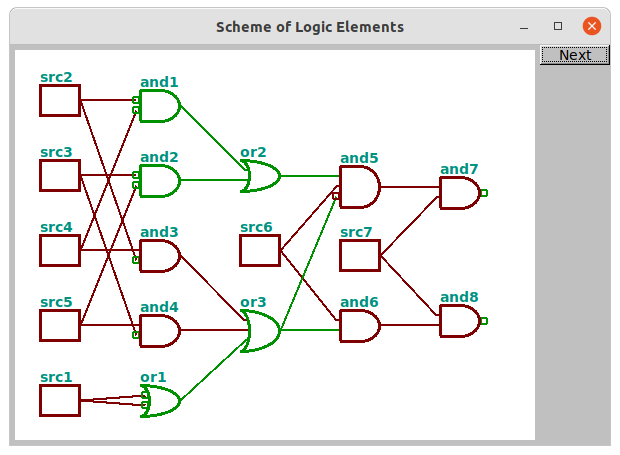
\includegraphics[width=0.6\textwidth]{images/logic_elements.png}

    }
    \caption{Пример рисования логической схемы}
    \label{fig:logicelems}
\end{figure}



%%========================
\paragraph{Анализ задачи.}
%%========================
Нам дан пример схемы с~логическими элементами. Нужно ответить на~следующие вопросы и сформулировать задачу.
\begin{enumerate}
    \item Какова предметная область?
    \begin{itemize}
        \item Работаем с~элементами математической логики.
    \end{itemize}

    \item В~каком контексте нужно разработать программный код?
    \begin{itemize}
        \item Необходим программный код, который позволяет смоделировать работу данной схемы.
        \item Этот код вполне вероятно будет использован для~моделирования подобных схем.
        \item Было бы удобно, если бы моделирование схемы не~зависело от~способа отображения процесса её работы (рисования).
    \end{itemize}

    \item Анализ исходных данных:
    \begin{itemize}
        \item На~схеме изображены не~все существующие логические элементы.
        \item На~схеме нет циклов.
        \item Вместо логического отрицания используются отрицания на~выходах/входах логических элементов.
    \end{itemize}
\end{enumerate}



%%=========================
\paragraph{Проектирование.}
%%=========================
Необходимо предусмотреть гибкость разрабатываемого программного кода.
\begin{itemize}
    \item Расширение функционала не~должно вынуждать полностью переписывать исходный код.
    \item Разделение на~небольшие части, подзадачи, которые могут быть использованы независимо (принцип <<разделяй и властвуй>>).
    \item Необходимо предусмотреть наиболее удобные уровни абстракции.
\end{itemize}

\bigskip Выделим в~коде две части:
\begin{itemize}
    \item Код для~непосредственного моделирования работы схемы.
    \item Код для~отображения процесса работы схемы (рисование).
\end{itemize}

\bigskip Продумаем примеры того, как бы мы хотели видеть использование разработанного программного кода:
\begin{enumerate}
    \item Создание элементов.
    \begin{itemize}
        \item При~создании логического элемента нужно указать его тип (тип объекта), инвертирован ли его выход (по~умолчанию не~инвертирован), задать \code{callback}-функцию (по~умолчанию \code{nullptr}).
        \item При~создании источника логического значения (сигнала) нужно указать это значение (по~умолчанию \code{false})
    \end{itemize}

    \item Соединение элементов.
    \begin{itemize}
        \item Соединений между логическими элементами гораздо больше, чем самих элементов.
        \item При~попытке сделать цикл в~схеме должно генерироваться исключение.
        \item Нужно предусмотреть (насколько это возможно) интуитивно понятный и лаконичный способ для~задания соединений.
        \item Удобно было бы соединять элементы по~цепочке.
        \item Будем использовать оператор \code{>>} для~соединения элементов (\code{and1 >> or2}).
        \item Подключение на~инвертированный вход вполне удобно смотрится с~использованием оператора~\code{\textasciitilde} (\code{or3 >> \textasciitilde{}and5}).
    \end{itemize}

    \item Изменение элементов.
    \begin{itemize}
        \item Для~задания логического значения источника удобно использовать оператор~\code{=}.
        \item Расчёт значений на~выходе каждого логического элемента должно происходить автоматически при~изменении состояния на~выходе элементов ниже по~цепочке.
        \item При~изменении состояния на~выходе элемента, этот элемент должен вызывать \code{callback}-функцию.
    \end{itemize}

    \item Получение значения на~выходе логического элемента.
    \begin{itemize}
        \item Оператор преобразования логического элемента в~значение \code{bool}.
    \end{itemize}

    \item Программный код для~отображения схемы и процесса её работы.
    \begin{enumerate}
        \item Нужно задавать только объекты, которые соответствуют логическим элементам на~схеме.
        \item Удобно создать класс-хранилище графических объектов SchemeShape.
        \item Отображение связей будет автоматическое, генерация объектов будет происходить в~SchemeShape.
        \item При~создании графических объектов нужно указать:
        \begin{itemize}
            \item на~какой схеме они расположены;
            \item какой логический элемент представляют;
            \item подпись (имя элемента);
            \item положение на~схеме.
        \end{itemize}
        \item Объект графического представления будет задавать \code{callback}-функцию для~элемента, который представляет.
        \item В~\code{callback}-функции будет происходить изменение цвета отображения элемента и связей.
    \end{enumerate}
\end{enumerate}



%%================
\WhatToReadSection
%%================
\textcite{Stroustrup:2016:ru}: \textbf{глава~10}



%%===============
\ExercisesSection
%%===============
\begin{exercise}
\item Выполните упражнения из~\textbookref{главы 9} учебника.

\end{exercise}

% !TEX encoding   = UTF8
% !TEX spellcheck = ru_RU
% !TEX root = ../seminars.tex

%%=============================
\chapter{Потоки ввода и вывода}
%%=============================

%%==========================
\section{Записи температуры}
%%==========================
Рассмотрим упражнение~2 из~\textbookref{главы~10}. Идею записи температуры выразим согласно тексту \textbookref{раздела~10.5} учебника:

\cppfile[firstline=9, lastline=13]{projects/09/store_temps.cpp}



%%========================
\paragraph{Запись в файл.}
%%========================
Легко написать функцию, которая сохранит готовые записи в~простом формате.

\cppfile[firstline=42, lastline=50]{projects/09/store_temps.cpp}

\noindent Тогда функция \code{main} может принять такой вид:

\cppfile[firstline=52, lastline=52]{projects/09/store_temps.cpp}
\cppfile[firstline=54, lastline=57]{projects/09/store_temps.cpp}



%%==========================
\paragraph{Тестовые данные.}
%%==========================
Попробуем генерировать температурные записи случайным образом. Для~правдоподобия зададим синусоидальное поведение в~течение дня. Примерно к~2 часам дня наблюдается максимум нагрева, а ночью земля остывает, и достигается минимум. Конечно, мы не~принимаем в~расчёт движение воздушных масс, облачность и прочее.

\begin{center}
  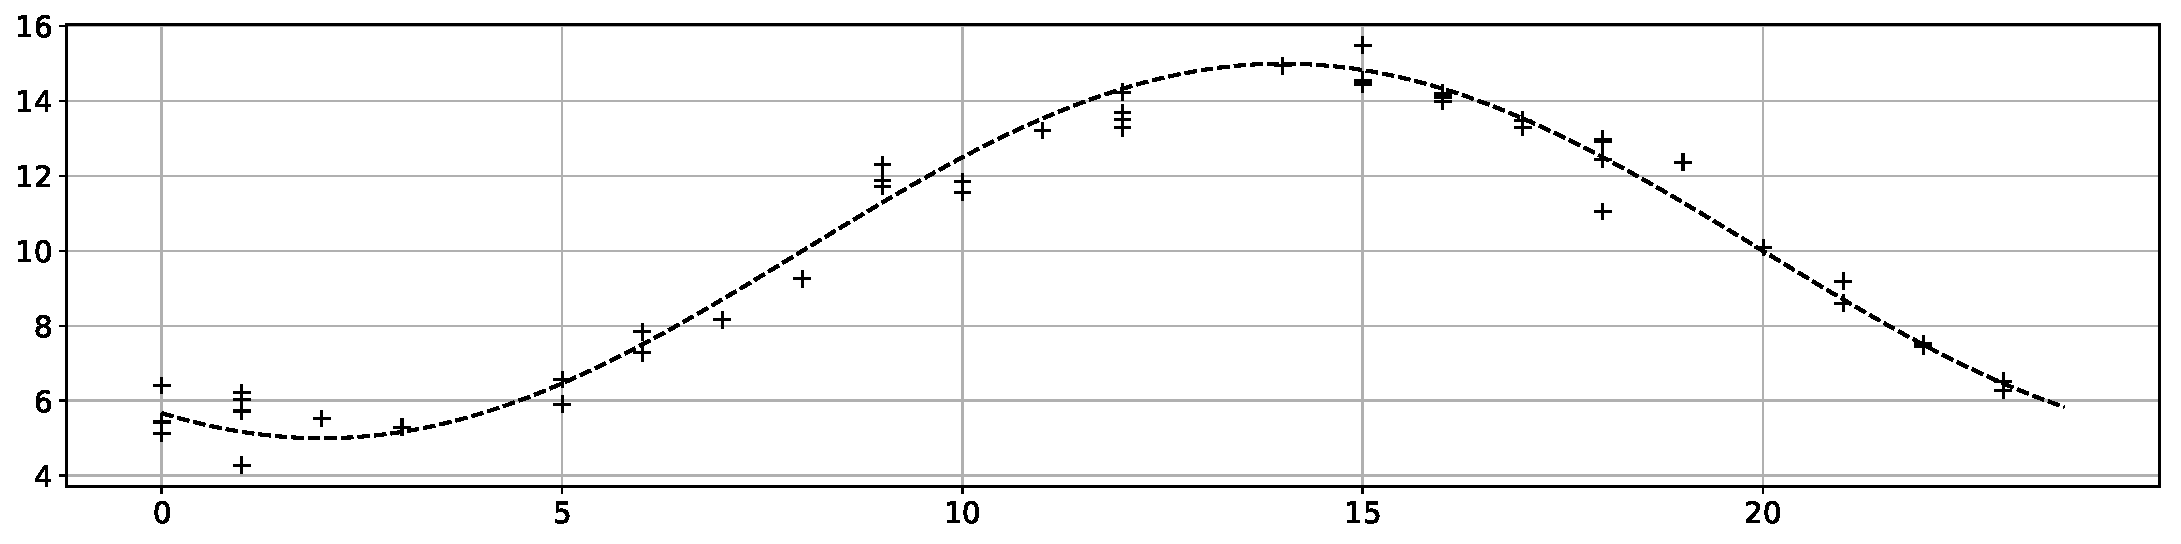
\includegraphics[width=0.8\textwidth]{images/raw_temps.pdf}
\end{center}

\cppfile[firstline=21, lastline=40]{projects/09/store_temps.cpp}

При~генерации записи мы случайным образом выбираем время суток, когда измерение произведено. А затем используем синусоиду с~некоторыми фиксированными параметрами: среднее в~течение дня, амплитуда колебаний за~день "--- для~вычисления текущего среднего значения и добавляем случайное отклонение по~нормальному закону распределения.



%%================================
\paragraph{Псевдослучайные числа.}
%%================================
Напомним, что функция плотности вероятности нормального распределения задаётся следующим соотношением:
\[
  p(x|\mu, \sigma) = \frac{1}{\sigma\sqrt{2\pi}} \cdot
                     \exp\left( -\frac{(x - \mu)^2}{2\sigma^2} \right)
\]
\noindent где \(\mu\) "--- среднее значение случайной величины \(x\), а \(\sigma\) "--- её стандартное отклонение. Величина \(\sigma\) означает, что с~вероятностью \(\approx 68\%\) значения \(x\) будут в~диапазоне \([\mu - \sigma, \mu + \sigma]\).

Рассмотрим определение функции, генерирующей псевдослучайное целое число в~заданном диапазоне из~заголовочного файла \code{std\_lib\_facilities.h}.

\cppfile[firstline=247, lastline=253]{projects/lib/std_lib_facilities.h}

По~аналогии, руководствуясь стандартом языка в~качестве справочника, пишем функцию генерирующую псевдослучайное число с~нормальным распределением.

\cppfile[firstline=15, lastline=19]{projects/09/store_temps.cpp}

\noindent Если необходимо генерировать различные последовательности псевдослучайных чисел при~разных запусках, следует задать произвольное начальное значение (\textenglish{seed}) генератору.

\begin{cppcode*}{linenos=false}
  static default_random_engine ran{time(nullptr)};
\end{cppcode*}



%%==========================
\paragraph{Чтение из файла.}
%%==========================
Продолжим работу с~записями и перейдём к~упражнению~3. Добавим оператор чтения из~потока ввода.

\cppfile[firstline=14, lastline=21]{projects/09/temp_stats.cpp}

\noindent
Заметьте, мы упустили из~вида проверку корректности входных данных! Добавьте её самостоятельно. После этого, записи можно прочитать из~файла следующим образом:

\cppfile[firstline=23, lastline=39]{projects/09/temp_stats.cpp}

\noindent
и организовать функцию \code{main} так:

\cppfile[firstline=65, lastline=65]{projects/09/temp_stats.cpp}
\cppfile[firstline=67, lastline=73]{projects/09/temp_stats.cpp}



%%==================
\section{Сортировка}
%%==================
Для~вычисления медианы нам понадобится упорядочить записи по~температуре. Выполним это, используя лямбда-выражение в~качестве критерия сортировки.

\cppfile[firstline=52, lastline=54]{projects/09/temp_stats.cpp}

Поскольку входные данные функции желательно не~изменять, а сортировка меняет порядок, нам понадобится копия вектора записей температур в~функции \code{temp\_stats}. Для~удобства инициализации этой копии, передадим её по~значению (!):

\cppfile[firstline=41, lastline=42]{projects/09/temp_stats.cpp}
\cpp`  // ...`
\cppfile[firstline=62, lastline=63]{projects/09/temp_stats.cpp}



%%========================
\section{Лямбда-выражения}\label{sect:lambda}
%%========================
Лямбда-выражения появились в~стандарте \lang{C++11} и немного доработаны в~более позднем \lang{C++14}. По своей сути, это автоматически генерируемые компилятором аналоги \emph{функторов} "--- объектов классов, которые имитируют поведение функций.

Теперь вы уже способны создать аналог нашего лямбда-выражения в~\lang{C++03} самостоятельно:

\begin{cppcode*}{linenos=false}
struct ReadingLess
{
  bool operator() (const Reading& a, const Reading& b) const
  {
    return a.temperature < b.temperature;
  }
};
\end{cppcode*}

Благодаря перегрузке оператора \code{()} имитируется поведение функции, то есть объект можно вызвать синтаксически точно так же, как обычную функцию. Отсюда и происходит название "--- функтор. Тело метода, определённого внутри класса, является подставляемым (\code{inline}), что обеспечивает эффективность для~коротких функций.

\begin{cppcode*}{linenos=false}
Reading a, b;
...
ReadingLess compare;
if (compare (a, b))  // behaves as an ordinary function here
  ...
\end{cppcode*}

\noindent
Вызов алгоритма сортировки в~стиле \lang{C++03}:

\cpp/sort (temps.begin(), temps.end(), ReadingLess());/

Очевидно, объект класса способен на~большее, чем просто функция. Он может хранить некоторое состояние и с~его помощью менять поведение функции-метода. А также инициализировать это состояние при~помощи конструкторов и обеспечить доступ к~нему через вспомогательные методы.

Часть лямбда-выражения с~квадратными скобками \code{[]} "--- это инициализирующий захват (\textenglish{capture}), реализация которого обеспечивается конструктором класса. Через него можно передавать копию (или ссылку) окружения лямбда-выражения. Подробнее эта тема раскрывается в~книге \cite{Stroustrup:2013:en}.

Лямбда-выражения коротко и ясно выражают идеи, определяются по~месту использования, широко применяются в~качестве аргументов для~алгоритмов библиотеки STL (\textenglish{Standard Template Library}) и могут быть размещены в~контейнерах. При~этом часть работы, а именно, определение класса, выполняет компилятор вместо нас. Именовать лямбда-выражение необязательно.



%%================
\WhatToReadSection
%%================
\textcite{Stroustrup:2016:ru}: \textbf{глава~11}



%%===============
\ExercisesSection
%%===============
\begin{exercise}
    \item Разработайте текстовый формат файла для~хранения схемы логических элементов (см.~страницу~\pageref{par:logic:v1}).

    \item Выполните упражнения из~\textbookref{главы~10} учебника.
\end{exercise}

% !TEX encoding   = UTF8
% !TEX spellcheck = ru_RU
% !TEX root = ../seminars.tex

%%================================
\chapter{Настройка ввода и вывода}
%%================================

%============================
\section{<<Переворот>> файла}
%============================
Рассмотрим упражнение~12 \textbookref{главы~11} учебника. Будем полагать, что файл может не~поместиться целиком в~оперативную память.

\cppfile[lastline=14]{projects/10/reverse_file.cpp}



%%===================================
\paragraph{Позиционирование в файле.}
%%===================================
Организуем считывание данных небольшими порциями по~\code{chunk} байтов из~начала файла (префикс \code{l} "--- left) и из~конца (префикс \code{r} "--- right) в~заготовленные буферы. Затем обратим порядок содержимого в~каждом буфере и запишем правый на~место левого, и наоборот "--- левый на~место правого. При~этом придётся управлять положением текущей позиции в~файле. Для~упрощения кода создадим два потока и откроем каждый для~доступа как на~чтение, так и на~запись одновременно.

\cppfile[firstline=16, lastline=54]{projects/10/reverse_file.cpp}

Контейнер \code{std::array} представляет собой обычный массив фиксированного размера. С~ним можно обращаться так же, как и с~динамическим массивом \code{std::vector}, т.\,е. доступны \code{size()}, \code{begin()}, \code{end()}, \code{empty()}, \code{[]}, \code{at()} и прочее, за~исключением методов меняющих размер.

\emph{Совет}: предпочитайте \code{std::array} взамен встроенных массивов в~стиле~\lang{C}.



%%==========================================
\paragraph{Аргументы функции \texttt{main}.}
%%==========================================
Вспомним, как мы запускаем какую-либо утилиту из~консоли и передаём ей аргументы, например:

\console`$ g++ -o bin/lsm -std=c++17 -pedantic -Wall -Wextra 02/least_squares.cpp`

\noindent \code{g++} "--- имя команды, а всё остальное "--- аргументы, которые ей передаёт пользователь. Если программа написана на~\code{C/C++}, то как она может получить эти аргументы? Для этого в~стандарте предусмотрен вариант функции \code{main} с~двумя аргументами:

\cppfile[firstline=56, lastline=56]{projects/10/reverse_file.cpp}

\noindent \code{argc} инициализируется количеством переданных аргументов. Имя команды является первым из~них и входит в~это число. А \code{argv} представляет собой массив значений.

Кто же вызывает \code{main} и передаёт ему эти аргументы? Среди звеньев цепочки, по~которой путешествуют наши аргументы, можно назвать сам командный интерпретатор и операционную систему, точнее, загрузчик на~исполнение.

Используя параметры командной строки, мы можем извлечь имена файлов и обратить порядок их содержимого в~теле функции \code{main}.

\cppfile[firstline=58, lastline=67]{projects/10/reverse_file.cpp}



%%======================
\paragraph{Тестирование}
%%======================
уже давно и прочно должно было войти в~привычку. Соберите исходный код в~исполнимый модуль

\console`$ g++ -o bin/reverse -std=c++14 -pedantic -Wall -Wextra 10/reverse_file.cpp`

\noindent и попробуйте <<сломать>> программку на~каких-нибудь входных данных. Вначале простые тесты, например:

\begin{consolecode}
$ echo "aaaaqbbbb" > 10/file.txt && bin/reverse 10/file.txt
$ cat 10/file.txt

bbbbqaaaa
\end{consolecode}

\noindent Команда \code{echo} просто печатает на~экран то, что ей передали. Далее, всё это перенаправляется с~экрана в~файл \code{file.txt}. Затем, обращается порядок и печатается на~экран новое содержимое файла при~помощи утилиты \code{cat}\footnote{Подробнее о~\name{Unix} утилитах, доступных в~\code{shell}, изложено в~Приложении на~странице \pageref{sect:utils}.}.

Заметьте, что \code{echo} добавила переход на~новую строку после выведенного текста, и теперь он оказался впереди. Рассмотрите разное количество символов, вплоть до~пустого файла: \code{"aqb"}, \code{"ab"}, \code{"a"}, \code{"}\code{"}. Убедившись, что всё работает, можно перейти к~исследованию варианта, когда размер файла больше порции, считываемой в~буфер за~один раз:

\console`$ bin/reverse 10/reverse_file.cpp 10/reverse_file.cpp`

\noindent Мы перевернули файл дважды и должны получить начальный вариант. Однако прежде, чем развлекаться с~исходным кодом, имеет смысл сохранить копию!

\console`$ cp 10/reverse_file.cpp 10/reverse_file_orig.cpp`

\noindent Фу-у-у-х! Теперь безопасно!

\begin{consolecode}
$ bin/reverse 10/reverse_file.cpp 10/reverse_file.cpp
$ diff -s 10/reverse_file.cpp 10/reverse_file_orig.cpp
Files 10/reverse_file.cpp and 10/reverse_file_orig.cpp are identical
\end{consolecode}



%%================
\WhatToReadSection
%%================
\textcite{Stroustrup:2016:ru}: \textbf{глава~12}



%%===============
\ExercisesSection
%%===============
\begin{exercise}
\item Выполните упражнения из~\textbookref{главы~11} учебника.

\end{exercise}

% !TEX encoding   = UTF8
% !TEX spellcheck = ru_RU
% !TEX root = ../seminars.tex

%%==============================
\chapter{Модель вывода на экран}
%%==============================

%%=======================================
\section{Сборка библиотеки \texttt{FLTK}}
%%=======================================
\todo{\ldots добавить описание\ldots}



%%=============================
\section{Графические примитивы}
%%=============================
Рассмотрим пример из~\textbookref{раздела~12.7}, использующий графические классы.

\begin{figure}[ht]
    {\centering
        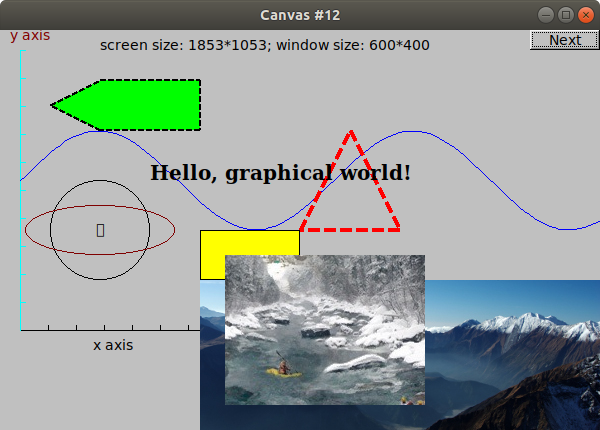
\includegraphics[width=0.6\textwidth]{images/shapes.png}

    }
    \caption{Окно программы c~графическими примитивами из~\textbookref{раздела~12.7}}
\end{figure}

\noindent Исходные файлы и проект программы размещены в~\href{\courserepourl}{репозитории}.

\begin{center}
    \code{projects/ch12/shape\_primitives}
\end{center}



%%=============
\paragraph{NB!}
%%=============
Использование директивы \code{using} приводит к~конфликту имён. В~системных графических библиотеках \name{Windows} определена функция \code{Rectangle}, а в~нашей графической библиотеке определён класс с~таким же именем. В~результате, компилятор обнаруживает неоднозначность определения имени.

Тем не~менее, поскольку все наши типы и функции размещены в~отдельном пространстве имён, следует просто уточнить, что мы имеем в~виду класс \code{Graph\_lib::Rectangle}.

\cppfile[firstline=1, lastline=10]{projects/ch12/shape_primitives/main.cpp}
\cppfile[firstline=12, lastline=21]{projects/ch12/shape_primitives/main.cpp}
\cpp`// ...`
\cppfile[firstline=48, lastline=51]{projects/ch12/shape_primitives/main.cpp}
\cpp`// ...`
\cppfile[firstline=113, lastline=113]{projects/ch12/shape_primitives/main.cpp}



%%=================================================
\section{Включение библиотеки \name{FLTK} в~проект}
%%=================================================
Рассмотрим внутренности проектного файла \code{CMakeLists.txt}, связанные с~добавлением внешней зависимости.

В~проект необходимо добавить файлы из~библиотеки \code{Graph\_lib}:

\cmakefile[firstline=22, lastline=23]{projects/ch12/shape_primitives/CMakeLists.txt}
\cmake'    # ...'
\cmakefile[firstline=25, lastline=28]{projects/ch12/shape_primitives/CMakeLists.txt}

\noindent которые будут подробно рассмотрены в~последующих \textbookref{главах} учебника. Классы этой библиотеки предоставляют нам сравнительно небольшой набор графических возможностей, реализованных на~основе библиотеки \name{FLTK}.

Система сборки \name{CMake} имеет механизмы поиска <<внешних>> библиотек в~системе. Это позволяет уменьшить зависимость описания проекта от~платформы, оставляя при~этом возможность вручную задать конкретные пути к~ним в~процессе конфигурации. Для поиска библиотеки \name{FLTK}, а также её зависимости "--- библиотеки более низкого уровня \name{OpenGL}, нужно добавить следующие строки:

\cmakefile[firstline=10, lastline=11]{projects/ch12/shape_primitives/CMakeLists.txt}

\noindent Флаг \code{REQUIRED} указывает, что без~данного компонента невозможна успешная сборка проекта. Таким образом, мы получаем более раннюю диагностику в~виде ошибки на~этапе конфигурирования.

\todo{\ldots добавить дальнейшее описание\ldots}



%%================
\paragraph{P.\,S.}
%%================
Подводя итоги, перечислим необходимые в проекте компоненты для сборки программы, которая использует сторонние библиотеки:
\begin{itemfeature}
    \item пути к заголовкам;
    \item пути к библиотекам;
    \item дополнительные флаги компилятору;
    \item библиотеки;
    \item дополнительные флаги компоновщику.
\end{itemfeature}
Эти возможности присутствуют в каждой более-менее приличной среде разработки. Однако способы их добавления зависят от конкретной среды и могут сильно отличаться. Необходимо изучать соответствующие руководства.



%%========================================================
\paragraph{Сборка в \name{Unix}-подобной командной среде.}
%%========================================================
Библиотека \name{FLTK} предоставляет удобную утилиту \code{fltk-config}, с помощью которой можно узнать необходимые настройки для сборки проекта, например:

\begin{consolecode}
$ fltk-config --cxxflags
-I/usr/local/include -I/usr/include/freetype2 -I/usr/include/libpng16 \
-D_LARGEFILE_SOURCE -D_LARGEFILE64_SOURCE -D_THREAD_SAFE -D_REENTRANT
$ fltk-config --ldflags
-L/usr/local/lib -lfltk -lXrender -lXcursor -lXfixes -lXext -lXft \
-lfontconfig -lXinerama -lpthread -ldl -lm -lX11
\end{consolecode}

\noindent и собрать исполняемый модуль программы:

\begin{consolecode}
$ g++ -o bin/shapes -std=c++14 -pedantic $(fltk-config --cxxflags) \
  projects/ch12/shape_primitives/main.cpp lib/Graph_lib/*.cpp \
  $(fltk-config --use-images --ldflags)
\end{consolecode}

Обратите внимание на использование конструкции \code{\$(command)} "--- аналог косых кавычек \code{`command`}. Командная среда вначале выполняет команду \code{command}, а затем подставляет на её место результат (то, что вывелось бы на экран) и запускает образовавшуюся в итоге команду.

Стандартный способ узнать возможности какой-либо утилиты "--- вызвать справку:
\console`$ fltk-config --help`%$

Теперь можно запустить нашу программу:
\console`$ bin/shapes`%$



%%==========================
\section{Элементы геометрии}\label{sect:geomelems}
%%==========================
Напишем ряд вспомогательных функций. Чтобы не загромождать основную программу и в дальнейшем иметь возможность использовать код повторно, разместим их в отдельном модуле (\code{lib/poly}): \code{poly.h}/\code{poly.cpp}.

Функция \code{regular\_polygon()} возвращает список вершин правильного \code{n}-угольника с центром в точке \code{center}, радиусом описанной окружности \code{radius} и начальным положением (углом) \code{angle} первой вершины, отсчитывая от оси X. Последний параметр позволяет задать необходимую ориентацию на плоскости нашего многоугольника. Положительное значение угла задаёт вращение против часовой стрелки. По умолчанию значение этого угла равно \code{0}.

\cppfile[firstline=17, lastline=32]{projects/lib/poly/poly.cpp}

\noindent
\parbox[c]{0.65\textwidth}{\parindent=1.25cm%
Изменение координат точки при вращении можно выразить через поворот самой системы координат:
\[
  \left\{ \begin{array}{l}
    x\prime = \phantom{-}x\cos\alpha + y\sin\alpha, \\
    y\prime =           -x\sin\alpha + y\cos\alpha.
  \end{array}\right.
\]
Используя эти соотношения, функция \code{rotated()} выполняет поворот точки \code{point} на угол \code{angle} относительно центра вращения \code{center} и возвращает новую точку. По умолчанию центр вращения расположен в начале координат.
}\hfill\parbox[c]{0.35\textwidth}{%
\begin{center}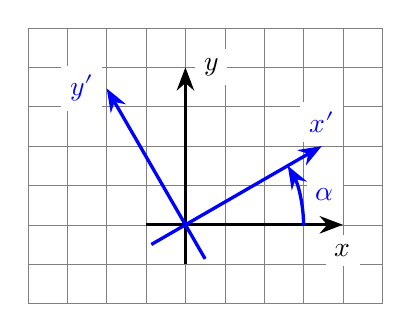
\begin{tikzpicture}[>=Stealth, very thick]
  \draw[help lines, step=.5cm] (-2, -1) grid (2.5, 2.5);
  \draw[->] (-0.5, 0) -- (2, 0) node[at end, below=3pt, fill=white] {\(x\)};
  \draw[->] (0, -0.5) -- (0, 2) node[at end, right=3pt, fill=white] {\(y\)};
  \draw[->, blue] (1.5, 0) arc [start angle=0, end angle=30, radius=1.5cm] node[midway, right=2pt, color=blue, fill=white] {\(\alpha\)};
  \draw[->, blue, rotate=30] (-0.5, 0) -- (2, 0) node[at end, above=1pt, color=blue, fill=white] {\(x\prime\)};
  \draw[->, blue, rotate=30] (0, -0.5) -- (0, 2) node[at end, left=1pt, color=blue, fill=white] {\(y\prime\)};
\end{tikzpicture}\end{center}
}% parbox

\cppfile[firstline=7, lastline=15]{projects/lib/poly/poly.cpp}

Функция \code{lerp()} добавлена в стандартную библиотеку \lang{C++20}. Она выполняет линейную интерполяцию между \(a\) и \(b\) для параметра \(t\) (или экстраполяцию, если \(t \notin [0, 1]\)).

\cppfile[firstline=30, lastline=30]{projects/lib/poly/poly.h}

Будет удобна ещё одна простая функция \code{append()}, которая добавит точки из списка в замкнутую ломаную \code{Closed\_polyline} из нашей графической библиотеки.

\cppfile[firstline=34, lastline=38]{projects/lib/poly/poly.cpp}

\noindent Здесь функция \code{as\_point()} преобразует вещественный радиус-вектор \code{Vec2d} в экранную точку \code{Point}, выполняя округление до целых значений по правилам математики.

\cppfile[firstline=32, lastline=35]{projects/lib/poly/poly.h}

\noindent Такое округление улучшает точность отрисовки линий на экране.



%%================
\section{Фракталы}
%%================
\emph{Фракталом} называется структура, состоящая из частей, которые в каком-то смысле подобны целому. Этот существенный отличительный признак наблюдается в эксперименте: фрактал выглядит одинаково, в каком бы масштабе его ни наблюдать. Взять хотя бы некоторые прекрасные кучевые облака. Они состоят из огромных <<горбов>>, на которых возвышаются <<горбы>> поменьше, на тех "--- <<горбы>> ещё меньше и т.д. вплоть до самого малого масштаба, который вы в состоянии разрешить.

\begin{figure}[ht]
    {\centering
        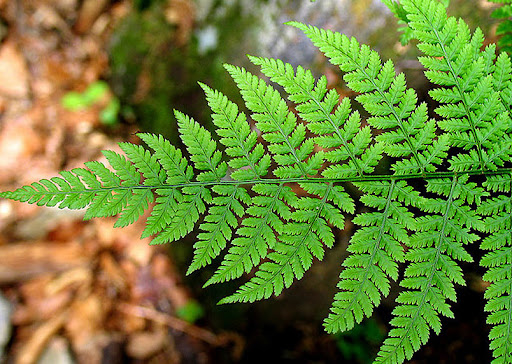
\includegraphics[height=0.26\textwidth]{images/fern.jpg}\hfil
        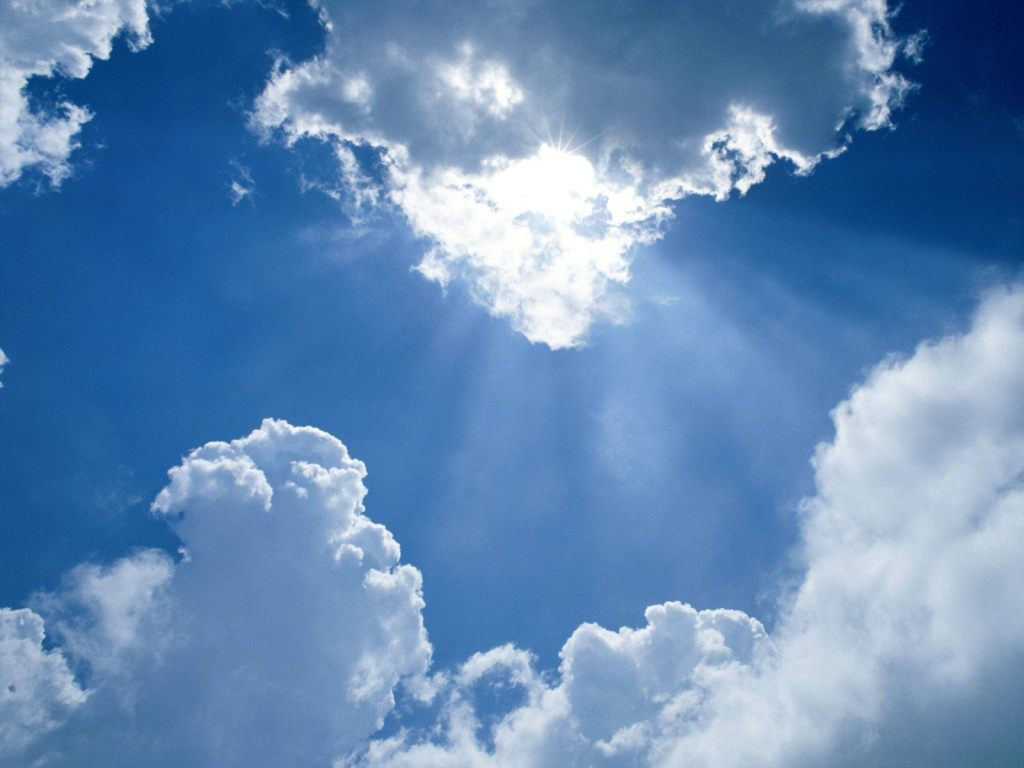
\includegraphics[height=0.26\textwidth]{images/clouds.jpg}\hfil
        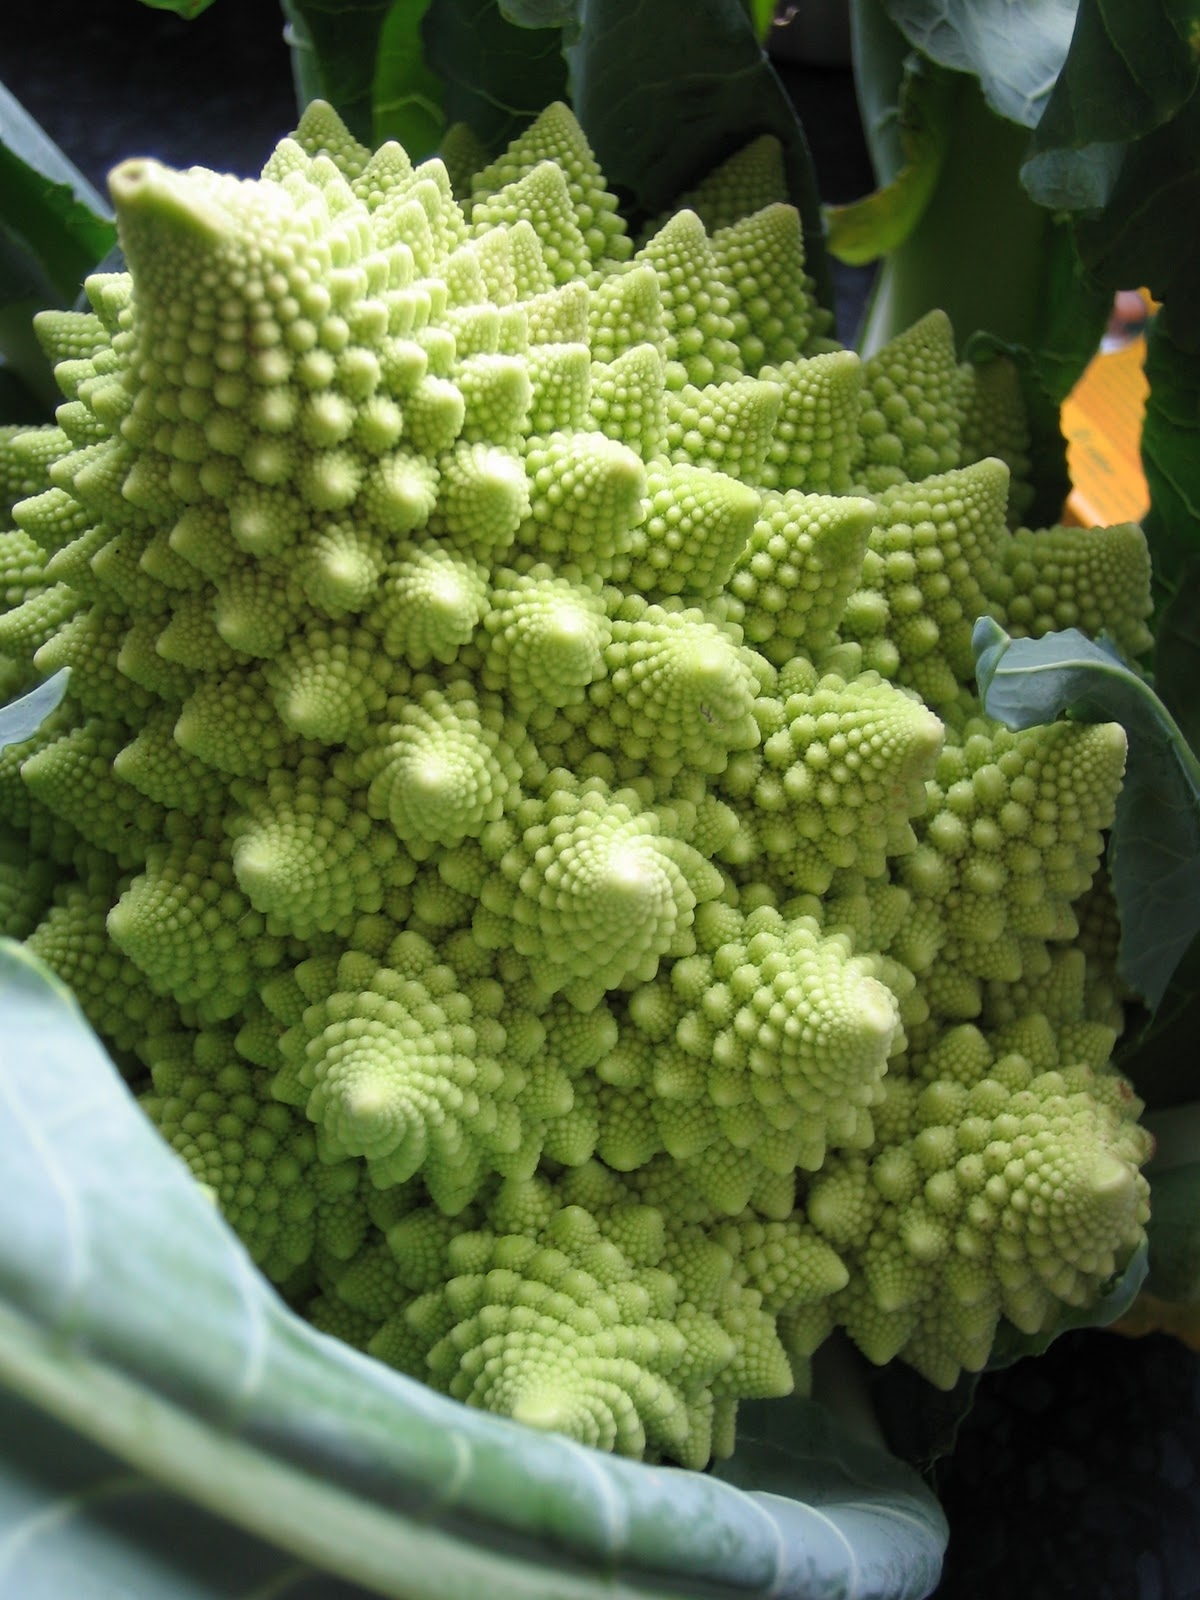
\includegraphics[height=0.26\textwidth]{images/romanesco_broccoli.jpg}

    }
    \caption{Примеры фракталов в природе}
\end{figure}



%%========================
\paragraph{Снежинка Коха,}
%%========================
построенная в виде замкнутой кривой на базе равностороннего треугольника, впервые была описана шведским математиком \href{https://ru.wikipedia.org/wiki/Кох,_Нильс_Фабиан_Хельге_фон}{Хельге фон Кохом} в 1904 году. В некоторых работах она получила название «остров Коха».

Доказано, что эта фрактальная кривая обладает рядом любопытных свойств. К примеру, длина её периметра равна бесконечности, что, однако, не мешает охватывать конечную площадь, величина которой равна \(\frac{8}{5}\) площади базового треугольника.

\begin{figure}[ht]
    {\centering
        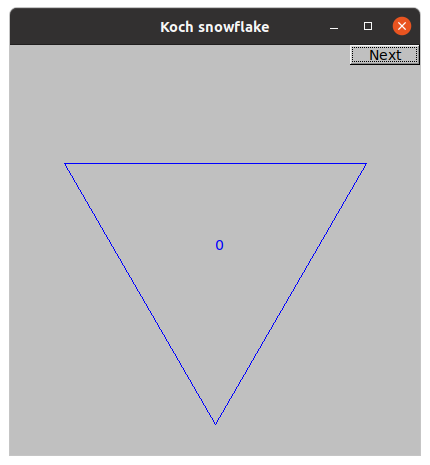
\includegraphics[width=0.3\textwidth]{images/koch_snowflake_n=0.png}\hfil
        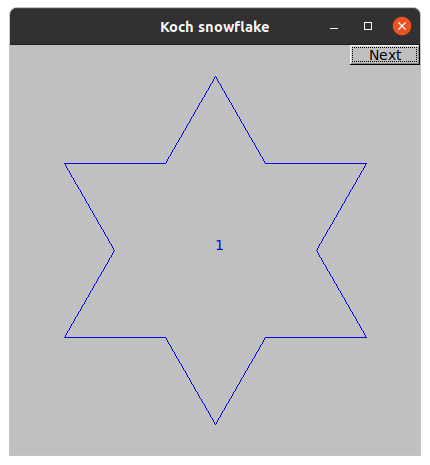
\includegraphics[width=0.3\textwidth]{images/koch_snowflake_n=1.png}\hfil
        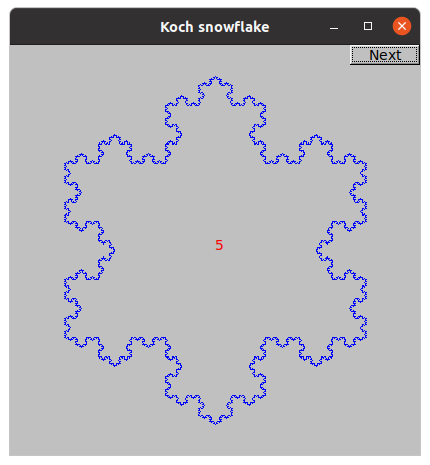
\includegraphics[width=0.3\textwidth]{images/koch_snowflake_n=5.png}

    }
    \caption{Снежинка Коха}
    \label{fig:kochshowflake}
\end{figure}

Построение кривой Коха начинается с прямолинейного отрезка единичной длины. Этот исходный отрезок называется \emph{затравкой} и может быть заменён каким-нибудь многоугольником, например, равносторонним треугольником или квадратом. Затравка "--- это \(0\)-е поколение кривой Коха. Далее, каждое звено затравки заменяется \emph{образующим элементом} "--- отрезок делится на 3 равные части и средняя часть заменяется равносторонним треугольником, у которого удалено основание (рисунок~\ref{fig:kochshowflake}).

Шаг этого алгоритма можно выразить следующим образом, используя ранее приведённые вспомогательные функции:

\cppfile[firstline=24, lastline=37]{projects/ch12/koch_snowflake/main.cpp}

Контейнер \code{std::list} представляет собой двусвязный список. Обойти его элементы можно используя итераторы "--- обобщённый аналог указателей. Они будут рассмотрены в \textbookref{главе~20} учебника. Список передаётся по rvalue-ссылке, которая позволяет избежать ненужного копирования объекта. Подробнее об этих ссылках и перемещении (\code{std::move}) мы узнаем в \textbookref{главе~18} учебника.

Вариант рисования снежинки Коха на базе правильного \code{n}-угольника в окне шириной~\code{w} средствами нашей библиотеки \code{Graph\_lib} можно записать так:

\cppfile[firstline=51, lastline=80]{projects/ch12/koch_snowflake/main.cpp}

Мы добавили текстовую метку в центре фигуры, показывающую номер шага алгоритма. И также учли, что дальнейшее измельчение кривой бессмысленно, если длина ребра становится менее~\(1\) пикселя. Функцию \code{max\_edge\_length()} предлагаем реализовать самостоятельно.

\textbf{NB!} Обратите особое внимание, что замкнутая ломаная создаётся в теле цикла каждый раз заново. Дело в том, что \code{Graph\_lib} не предоставляет удобного способа добавления новых точек в середину кривой. Мы вынуждены откреплять нашу кривую от окна в конце итерации, чтобы избежать отрисовки несуществующего объекта.


%=================
% !TEX encoding   = UTF8
% !TEX spellcheck = ru_RU
% !TEX root = ../seminars.tex

%%=================================
\section{Правильные многоугольники}
%%=================================
Нарисуем ряд вложенных правильных многоугольников из~упражнения~11 \textbookref{главы~12}.

\begin{figure}[ht]
  {\centering
    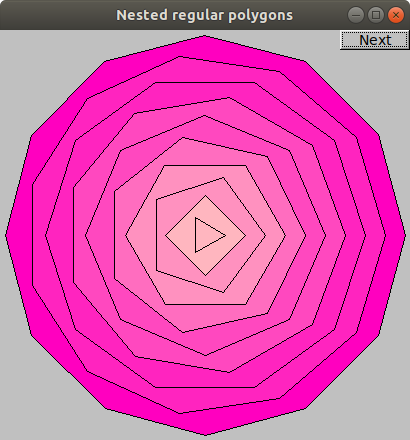
\includegraphics[height=0.3\textwidth]{images/regular_polygons.png}

  }
  \caption{Вложенные правильные многоугольники}
  \label{fig:regpoly}
\end{figure}

Покажем лишь ключевой фрагмент кода. Напомним, что функция \code{regular\_polygon()} вычисляет вершины правильного многоугольника и была представлена ранее в~разделе~\ref{sect:geomelems}.

\cppfile[firstline=19, lastline=45]{projects/ch12/regular_polygons.cpp}

Класс \code{Vector\_ref} рассматривается в~\textbookref{главе~13} и удобен для~хранения множества неименованных объектов. Многоугольники рисуются с~использованием вращательной симметрии и раскрашиваются в~оттенки пурпурного (см. диаграмму цветов из~\textbookref{главы~13}). Результат работы программы показан на~рисунке~\ref{fig:regpoly}.



%%====================
\section{Суперэллипсы}
%%====================
Суперэллипс, также известный как кривая Лямэ, названная в~честь \href{https://en.wikipedia.org/wiki/Gabriel_Lam\%C3\%A9}{Габриэля Лямэ}, "--- замкнутая кривая, которая как и эллипс обладает большой и малой полуосями, а также симметрией относительно них, но в~общем случае другой формой.

\begin{figure}[ht]
  {\centering
    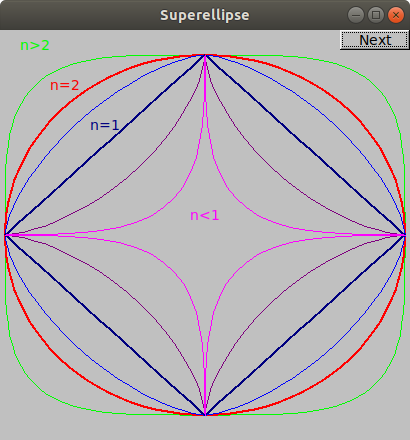
\includegraphics[height=0.3\textwidth]{images/superellipse.png}

  }
  \caption{Суперэллипсы}
  \label{fig:superellipse}
\end{figure}

В~декартовой системе координат суперэллипс в~обобщённом виде задаётся следующим соотношением:
\[
  \left| \frac{x}{a} \right|^m + \left| \frac{y}{b} \right|^n = 1;\quad m, n > 0.
\]

В~параметрическом виде, где параметр~\(t\) не~имеет никакой геометрической интерпретации, кривая выражается системой уравнений:
\begin{equation}
  \label{eq:superellipse}
  \left\{\begin{array}{l}
    x(t) = a\,\mathrm{sign}(\cos t) \cdot |\cos t|^{\frac{2}{m}},\\
    y(t) = b\,\mathrm{sign}(\sin t) \cdot |\sin t|^{\frac{2}{n}};
  \end{array}\right.
  \quad 0 \leqslant t \leqslant 2\pi.
\end{equation}

Функция, добавляющая точки, лежащие на~суперэллипсе, по~формуле~(\ref{eq:superellipse}), приведена ниже:

\cppfile[firstline=20, lastline=35]{projects/ch12/superellipse.cpp}

Функцию, определяющую знак числа, можно написать таким образом:

\cppfile[firstline=18, lastline=18]{projects/ch12/superellipse.cpp}

Ключевой фрагмент функции \code{main()} для~рисования нескольких вложенных суперэллипсов из~упражнения~12 \textbookref{главы~12}:

\cppfile[firstline=40, lastline=54]{projects/ch12/superellipse.cpp}

Мы уверены, что вы сможете самостоятельно добавить текстовые метки (подписи) к~кривым и раскрасить их, например, как на~рисунке~\ref{fig:superellipse}.

%=================



%%================
\WhatToReadSection
%%================
\textcite{Stroustrup:2016:ru}: \textbf{глава~13}



%%===============
\ExercisesSection
%%===============
\begin{exercise}
\item Выполните упражнения из \textbookref{главы~12} учебника.

\item Постройте так называемую антиснежинку Коха. Алгоритм генерирования заключается в вырезании на каждом этапе всё новых и новых треугольников из исходного многоугольника. Иными словами, рёбра базовой формы модифицируются внутрь, а не наружу. В результате полученная фигура охватывает бесконечное множество несвязанных областей.

\begin{figure}[ht]
  {\centering
    
\includegraphics[height=0.2\textwidth]{images/koch_curve_85_degrees.png}

  }
  \caption{Фрактал Цезаро "--- вариант кривой Коха с углом между \(60^{\circ}\) и \(90^{\circ}\) (\(85^{\circ}\))}
\end{figure}

\item Нарисуйте дракона Хартера, также известного как дракона Хартера--Хейтуэя. Он был впервые исследован физиками \name{NASA} "--- Джоном Хейтуэем (John Heighway), Брюсом Бэнксом (Bruce Banks), и Вильямом Хартером (William Harter). В 1967 году описан Мартином Гарднером в колонке «Математические игры» журнала <<\textenglish{Scientific American}>>. Многие из свойств фрактала были описаны Чендлером Дэвисом (Chandler Davis) и Дональдом Кнутом.

\begin{figure}[ht]
  \begin{center}
    \fbox{\begin{minipage}{0.4\textwidth}
      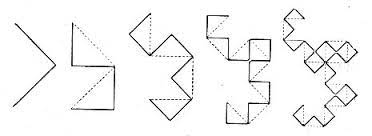
\includegraphics[width=\textwidth]{images/harter-heighway_dragon_steps-1.jpg}\\
      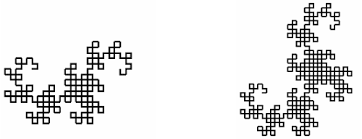
\includegraphics[width=\textwidth]{images/harter-heighway_dragon_steps-2.png}
    \end{minipage}}
    \hfil
    \fbox{\begin{minipage}{0.25\textwidth}
      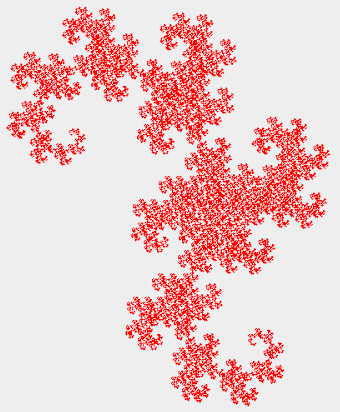
\includegraphics[width=\textwidth]{images/harter-heighway_dragon.png}
    \end{minipage}}
  \end{center}
  \caption{Дракон Хартера--Хейтуэя}
\end{figure}

\end{exercise}

%% !TEX encoding   = UTF8
% !TEX spellcheck = ru_RU
% !TEX root = ../seminars.tex

%%==========================
\chapter{Графические классы}
%%==========================
В~качестве образца приведём несколько примеров решения упражнений. Выполняя некоторые упражнения, мы по~сути расширяем графическую библиотеку, поэтому включим все новые классы в~пространство имён \code{Graph\_lib}. Весь этот код разместим в~каталоге \code{projects/lib/Graph\_lib/ext}. Заголовки и определения классов в~файле \code{graph.h}:

\cppfile[lastline=2, linenos=false]{projects/lib/Graph_lib/ext/graph.h}
\cpp`// ... (standard headers)`
\cppfile[firstline=6, lastline=8, linenos=false]{projects/lib/Graph_lib/ext/graph.h}
\cpp`// ... (extension classes)`
\cppfile[firstline=81, linenos=false]{projects/lib/Graph_lib/ext/graph.h}

\noindent а реализацию функций "--- в~\code{graph.cpp}:

\cpp`// ... (standard headers)`
\cppfile[firstline=4, lastline=6, linenos=false]{projects/lib/Graph_lib/ext/graph.cpp}
\cpp`// ... (methods implementation)`
\cppfile[firstline=187, linenos=false]{projects/lib/Graph_lib/ext/graph.cpp}



%%===================
\section{Дуга (арка)}
%%===================
Рассмотрим класс \code{Arc} для~рисования дуги (или арки) из~упражнения~1 \textbookref{главы~13}. Дуга должна быть частью эллипса. Соответственно, разумно в~качестве базового класса выбрать \code{Ellipse}. Это позволит использовать часть уже разработанной функциональности.

\begin{figure}[ht]
    {\centering
        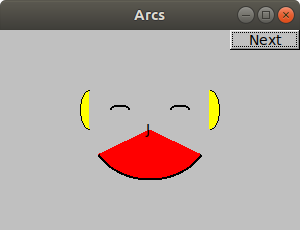
\includegraphics[height=0.25\textwidth]{images/arc.png}~\textit{a})
        \hfil
        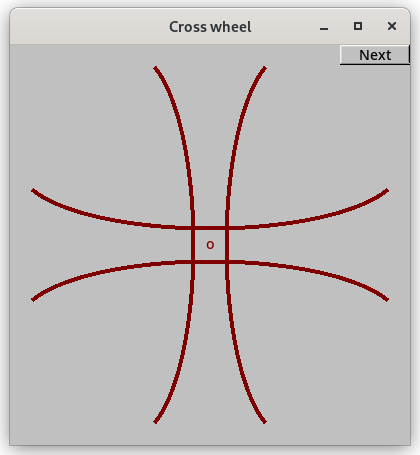
\includegraphics[height=0.25\textwidth]{images/cross_wheel.png}~\textit{б})
        \hfil
        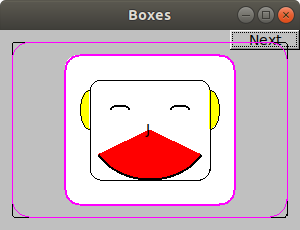
\includegraphics[height=0.25\textwidth]{images/box.png}~\textit{в})

    }
    \caption{Рожицы из~арок и мальтийский крест}
    \label{fig:arc}
\end{figure}

\cppfile[firstline=10, lastline=29]{projects/lib/Graph_lib/ext/graph.h}

\noindent
Ограничений на~начальный и конечный углы дуги мы не~накладываем.

В~конструкторе необходимо инициализировать часть, соответствующую базовому классу \code{Ellipse}, а затем углы, которые мы добавили для~арки:

\cppfile[firstline=8, lastline=11]{projects/lib/Graph_lib/ext/graph.cpp}

В~наиболее сложной части, а именно, отрисовке фигуры, мы взяли за~основу функцию из~класса \code{Ellipse}. Всё, что нужно, "--- это изменить углы:

\cppfile[firstline=13, lastline=26]{projects/lib/Graph_lib/ext/graph.cpp}

Теперь мы можем нарисовать рожицу из~нескольких дуг, используя класс \code{Arc}, например, как показано на~рисунке~\ref{fig:arc}\textit{a}. Нос добавлен при~помощи метки \code{Mark}.



%%============================================
\section{Прямоугольник с~закруглёнными углами}
%%============================================
Теперь рассмотрим класс \code{Box} из~упражнения~2 \textbookref{главы~13}. Он очень похож на~обычный прямоугольник. Единственное, что необходимо добавить, "--- радиус скругления углов. После не~слишком удачной реализации с~хранением четырёх линий в~объекте \code{Lines} и четырёх дуг в~массиве из~объектов \code{Arc}, мы решили наследовать от~\code{Rectangle}:

\cppfile[firstline=32, lastline=51]{projects/lib/Graph_lib/ext/graph.h}

Если пользователь не~указал радиус скругления, мы решили по~умолчанию задать величину 10\,\% от~наименьшей стороны. Это удобно. Но поскольку эта величина известна только на~этапе выполнения, необходим некий трюк. Мы задали в~качестве значения по~умолчанию (константа \code{automatic}) наибольшее целое число, представимое типом \code{int} (необходим заголовок \code{<limits>}).

Реализация первого конструктора довольно проста, отрицательные радиусы скругления мы отбрасываем:

\cppfile[firstline=28, lastline=36]{projects/lib/Graph_lib/ext/graph.cpp}

Второй конструктор совершенно аналогичен. Следует инициализировать базовую часть "--- класс \code{Rectangle} "--- двумя угловыми точками, а для~получения длины и ширины в~теле конструктора можно воспользоваться методами \code{width()} и \code{height()}.

Функция изменения радиуса скругления \code{set\_roundness()} также должна выполнить проверку на~неотрицательность аргумента, после чего присвоить новый радиус.

Стоит уделить внимание отрисовке. Она несколько сложнее, чем для~арки или прямоугольника, особенно, если добавить поддержку заливки фигуры цветом. Код функции представлен ниже:

\cppfile[firstline=47, lastline=54]{projects/lib/Graph_lib/ext/graph.cpp}
\cpp`    // ... use fl_pie() and fl_rectf()`
\cppfile[firstline=67, lastline=83]{projects/lib/Graph_lib/ext/graph.cpp}

Добавим контуры нашей рожице и несколько рамок с~разным скруглением, используя класс \code{Box}, например, как показано на~рисунке~\ref{fig:arc}\textit{в}.



%%================
% !TEX encoding   = UTF8
% !TEX spellcheck = ru_RU
% !TEX root = ../seminars.tex

%%================================
\section{Правильный шестиугольник}
%%================================
Рассмотрим класс \code{Regular\_hexagon} из~упражнения~8 \textbookref{главы~13}. Правильный шестиугольник, по~сути, является многоугольником \code{Polygon}. Однако он не~может содержать количество вершин, отличное от~6-ти. Таким образом, заманчиво наследовать от~\code{Polygon}, но тогда функцию \code{add()}, добавляющую дополнительные точки, необходимо как-то исключить из~интерфейса. И хотя, в~принципе, некоторые языки (с~динамической типизацией) позволяют сделать это, наследование интерфейса нарушилось бы. То есть там, где требуется \code{Polygon} мы не~смогли бы использовать \code{Regular\_hexagon}, в~который нельзя добавлять точки.

Хоть это лишает нас возможности воспользоваться реализацией классов \code{Polygon} или \code{Closed\_polyline}, \emph{логически правильным} решением является наследовать от~абстрактной фигуры \code{Shape}:
\cppfile[firstline=49, lastline=61]{projects/lib/Graph_lib/ext/graph.h}

В~конструкторе добавляем точки, используя вращательную симметрию:
\cppfile[firstline=99, lastline=113]{projects/lib/Graph_lib/ext/graph.cpp}

\noindent Округление при~помощи функции \code{std::round()} вместо отбрасывания дробной части даёт возможность слегка улучшить качество рисования в~отдельных случаях.

В~реализации следующих методов, которые предоставляются для~удобства пользователей, применяется априорное знание об~ориентации шестиугольника на~плоскости:
\cppfile[firstline=115, lastline=133]{projects/lib/Graph_lib/ext/graph.cpp}

Заметим, что эти функции можно было бы вынести из~класса, то есть сделать внешними по~отношению к~классу. Тем не~менее, мы расположили их внутри, поскольку это свойства самих объектов и эти свойства есть у~подобных объектов других типов. Например, у~окна также есть длина (\code{x\_max()}) и ширина (\code{y\_max()}).

Код оставшейся функции \code{draw\_lines()} в~точности повторяет реализацию из~классов \code{Open\_polyline} и \code{Closed\_polyline}:
\cppfile[firstline=135, lastline=157]{projects/lib/Graph_lib/ext/graph.cpp}

Пример рисования правильных шестиугольников показан на~рисунке~\ref{fig:regularhexagon}.



%%==================================
\section{Мозаика из~шестиугольников}
%%==================================
Применим разработанный класс \code{Regular\_hexagon} для~рисования мозаики в~пределах прямоугольной области из~упражнения~9 \textbookref{главы~13}.

\begin{figure}[ht]
  {\centering
    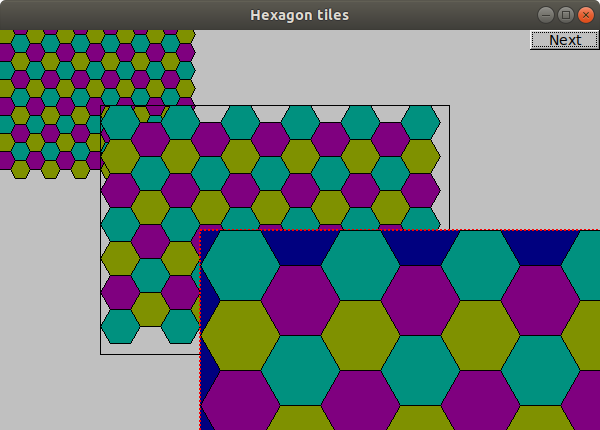
\includegraphics[width=0.6\textwidth]{images/hexagon_tiles.png}

  }
  \caption{Элементы мозаики из~правильных шестиугольников}
  \label{fig:regularhexagon}
\end{figure}

Наследование выполним от~класса \code{Rectangle}, а для~хранения множества правильных шестиугольников воспользуемся классом \code{Vector\_ref}:

\cppfile[firstline=64, lastline=76]{projects/lib/Graph_lib/ext/graph.h}

Вся работа по~формированию мозаики выполняется в~конструкторе. Параметры~\code{p}, \code{ww} и~\code{hh} задают прямоугольник, который заполняется одинаковыми правильными шестиугольниками. Размер шестиугольников определяется радиусом описанной окружности \code{rr}. Код конструктора приведён ниже:

\cppfile[firstline=160, lastline=190]{projects/lib/Graph_lib/ext/graph.cpp}

\begin{figure}[ht]
  {\centering
    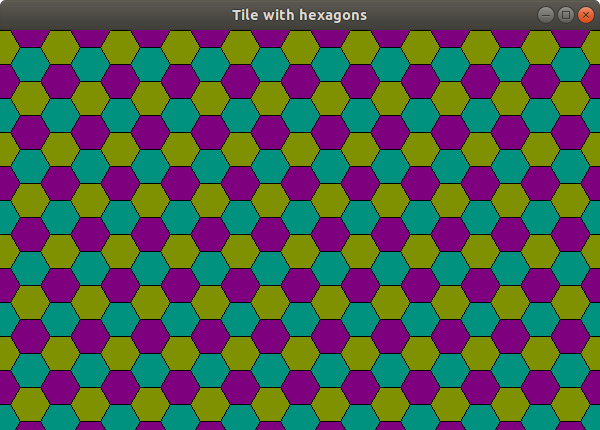
\includegraphics[width=0.6\textwidth]{images/tile_window.png}

  }
  \caption{Окно, полностью заполненное мозаикой}
  \label{fig:hexagontile}
\end{figure}

Реализация перекрывающих методов выполняется тривиально:

\cppfile[firstline=192, lastline=204]{projects/lib/Graph_lib/ext/graph.cpp}

В~начале мы рисуем прямоугольник, затем мозаику. По~умолчанию, прямоугольник не~рисуется. Это поведение мы установили в~конструкторе класса, задав невидимый цвет. Если изменить цвет рисования, то мы увидим границу (и заливку) прямоугольной области, как показано на~рисунке~\ref{fig:regularhexagon}. На~рисунке~\ref{fig:hexagontile} мозаикой покрыта вся область окна.

%%================



%%================
\WhatToReadSection
%%================
\textcite{Stroustrup:2016:ru}: \textbf{глава~14}



%%===============
\ExercisesSection
%%===============
\begin{exercise}
\item Выполните упражнения из~\textbookref{главы~13} учебника.

\begin{figure}[ht]
    {\centering
        \hfill
        \subbottom[Спираль Дюрера\label{fig:spirals:a}]{%
            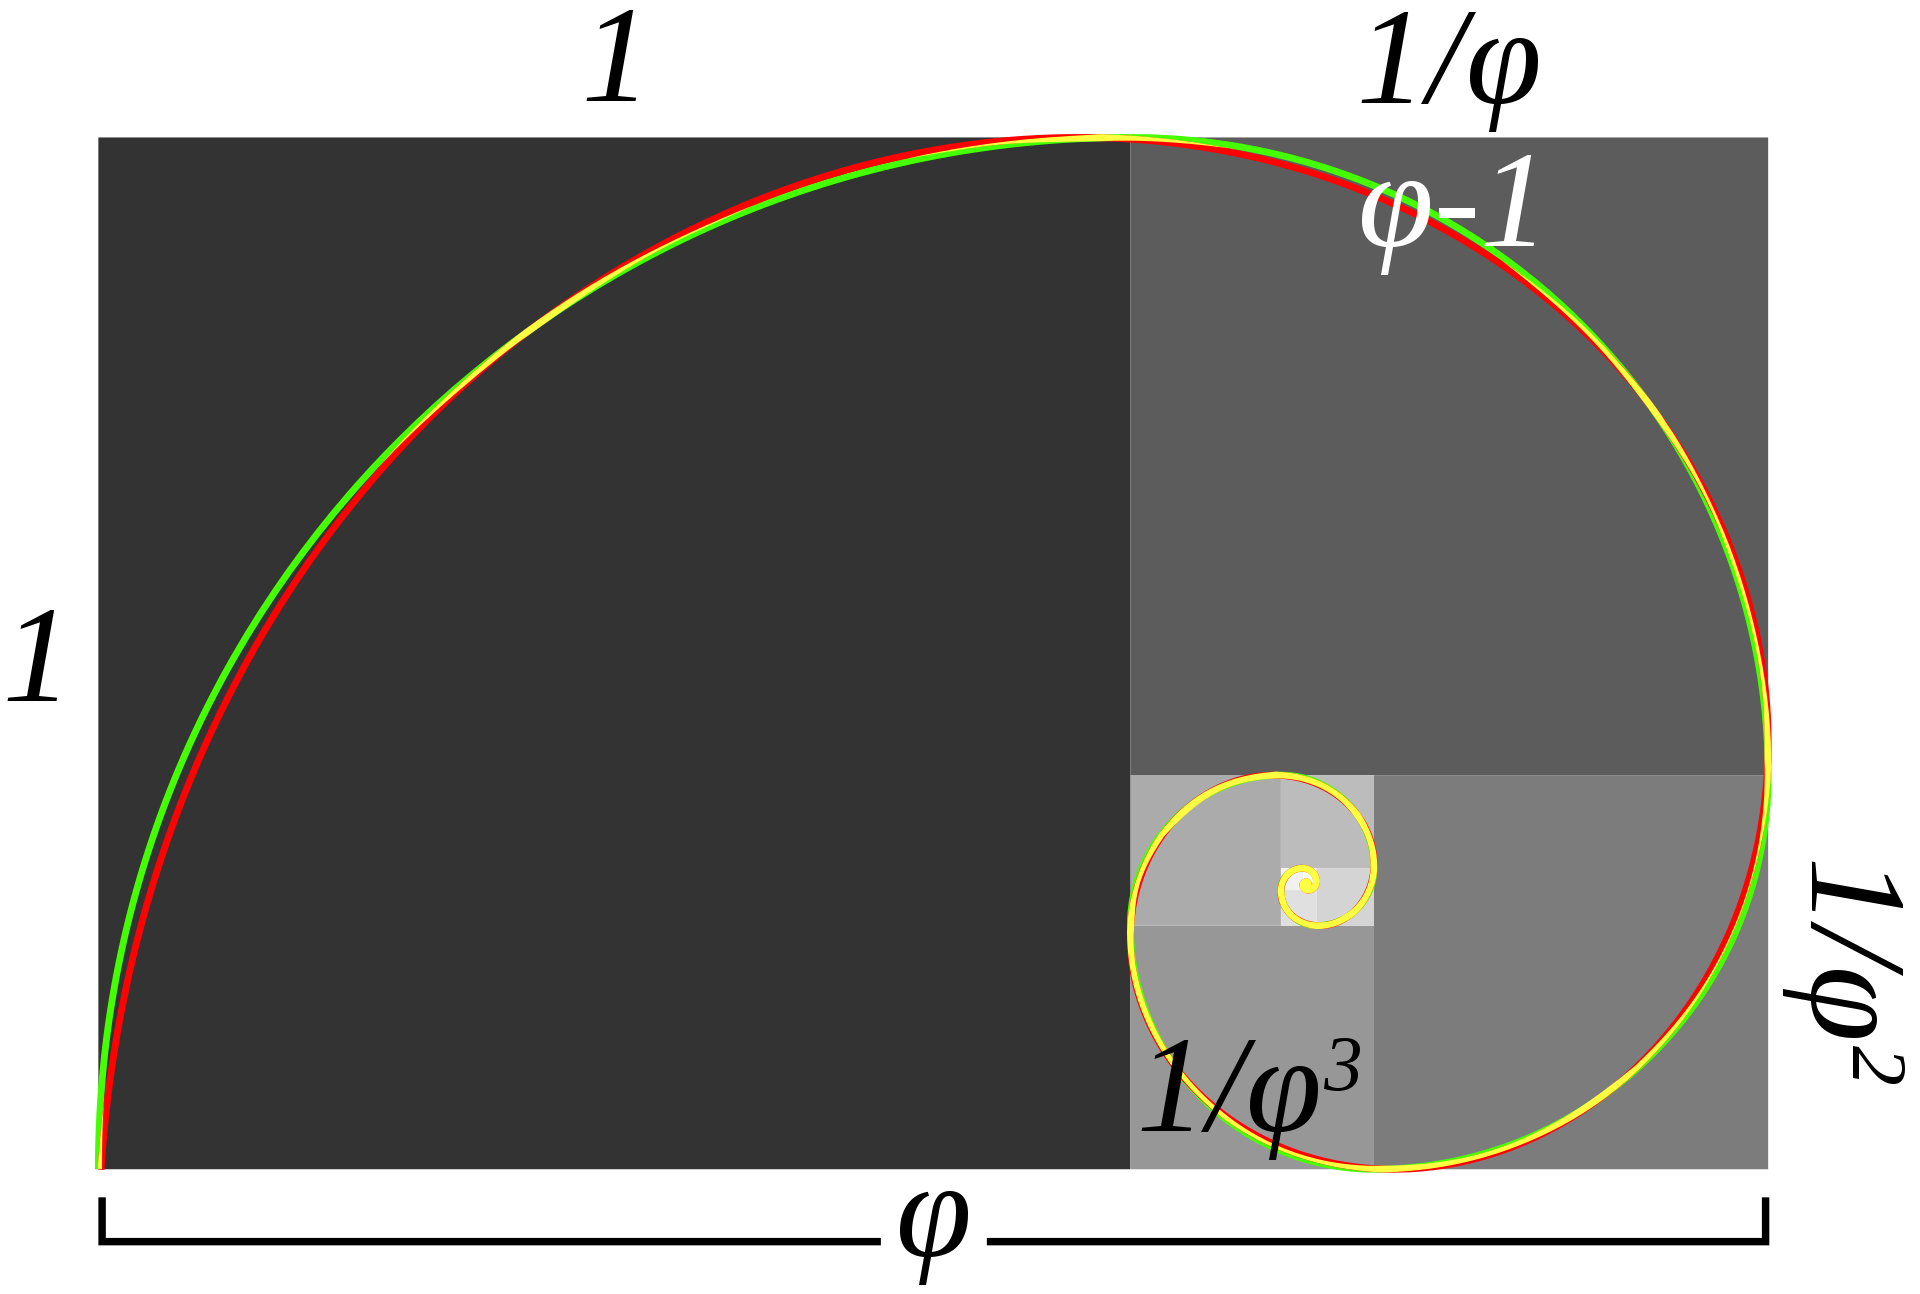
\includegraphics[height=0.25\textwidth, frame]{images/fake_real_log_spiral.png}}
        \hfill
        \subbottom[Спираль Фибоначчи\label{fig:spirals:b}]{%
            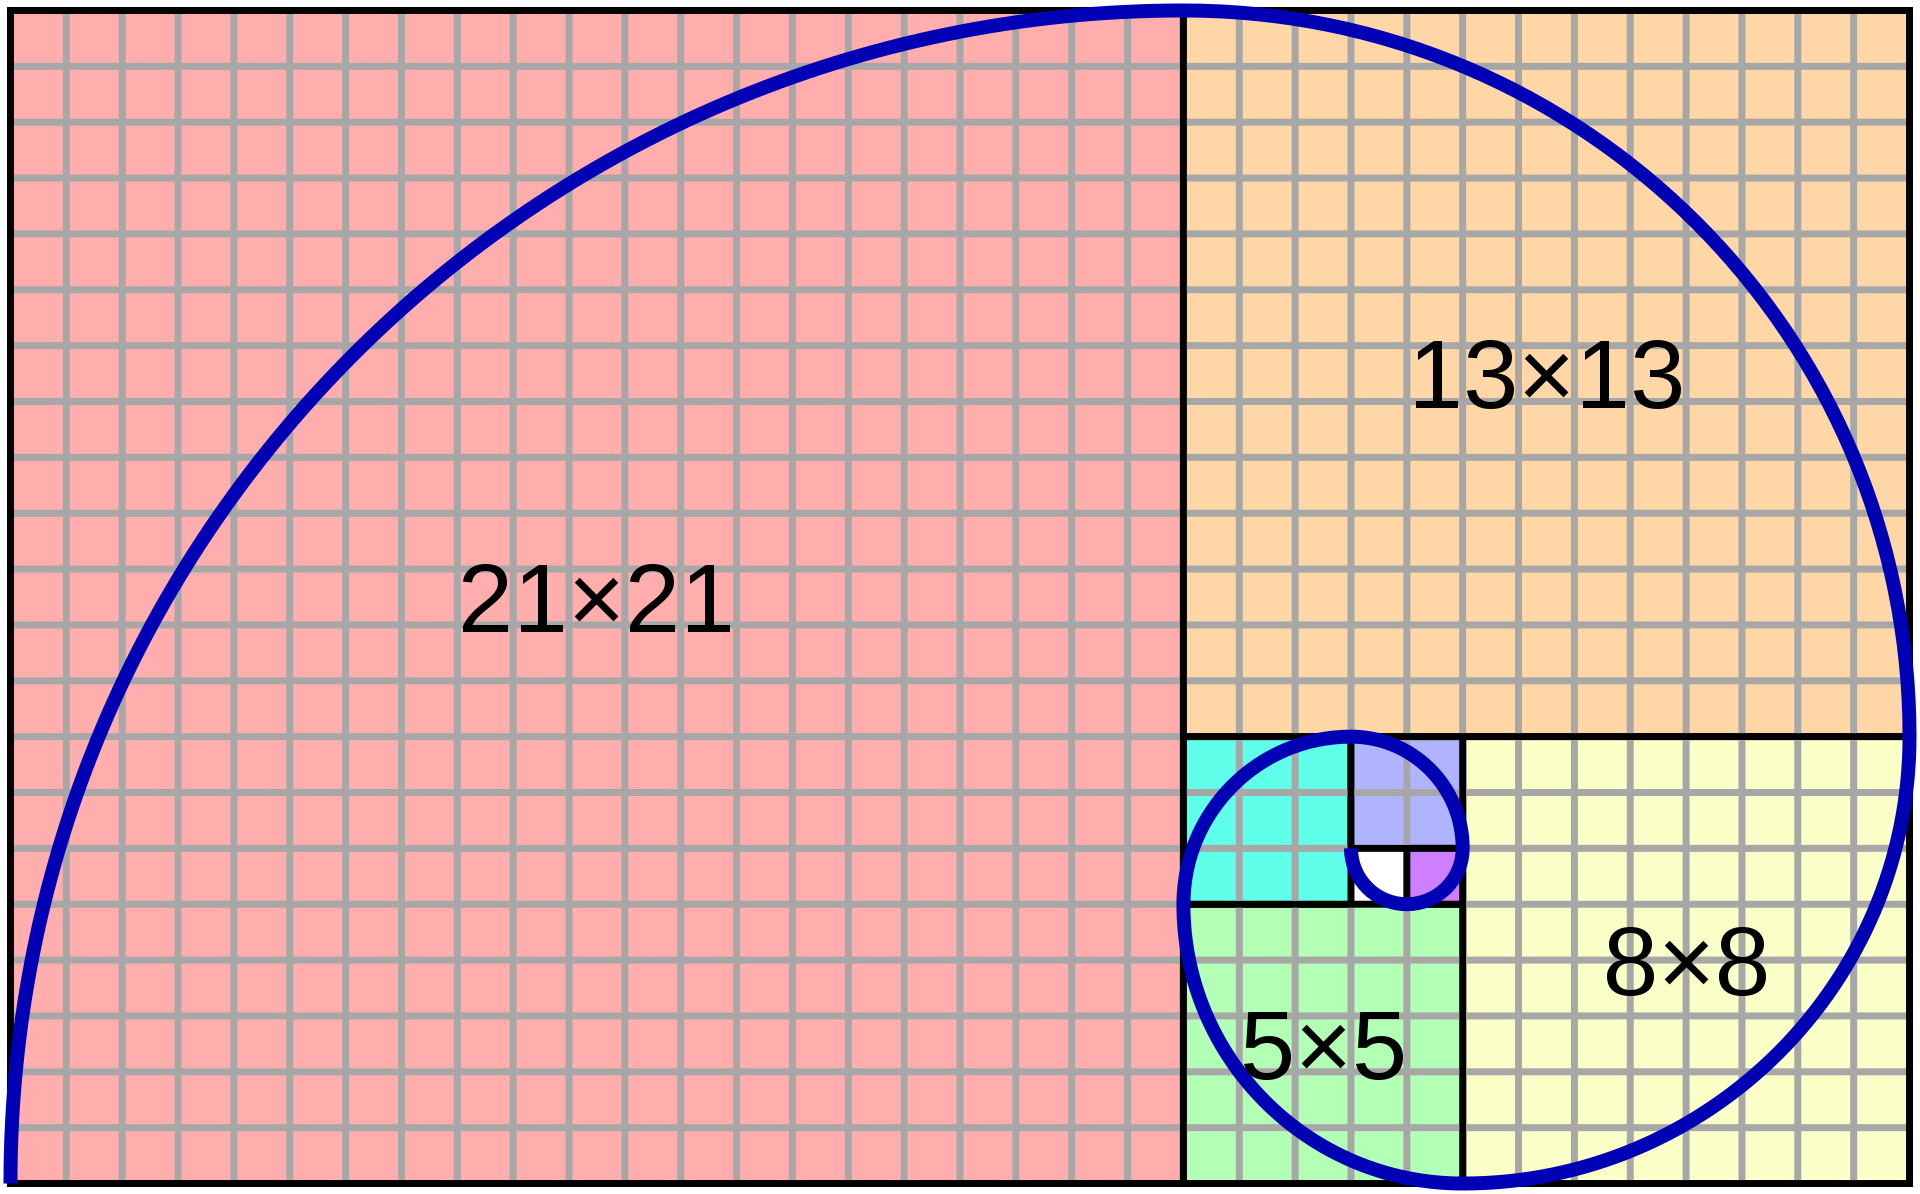
\includegraphics[height=0.25\textwidth]{images/fibonacci_spiral.png}}
        \hfill
    }
    \caption{Приближения золотой спирали}
    \label{fig:spirals}
\end{figure}

\item При~вписывании \emph{золотой спирали} в~последовательность вложенных друг в~друга золотых прямоугольников, она аппроксимируется спиралью, построенной по~методу Дюрера. Золотой прямоугольник можно разделить на~квадрат и подобный ему прямоугольник, его, в~свою очередь, разделить тем же образом, и продолжать этот процесс произвольное число раз. Если в~эти квадраты вписать соединенные между собой четвертинки окружностей, то получается спираль, изображённая на~рисунке~\ref{fig:spirals:a} зелёным цветом.

\smallskip

Спираль Фибоначчи строится подобно вышеописанной спирали, за~исключением того, что начинают с~прямоугольника из~двух квадратов и добавляют потом к~большей стороне прямоугольника квадрат такой же длины. Поскольку отношение между соседними числами Фибоначчи стремится к~золотой пропорции, спираль всё больше приближается к~золотой спирали по~мере добавления квадратов.

\begin{figure}[ht]
    {\centering
        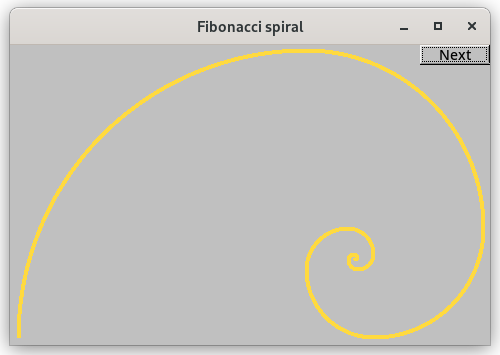
\includegraphics[height=0.25\textwidth]{images/fibonacci_spiral_draw.png}
        \hspace{1.5cm}
        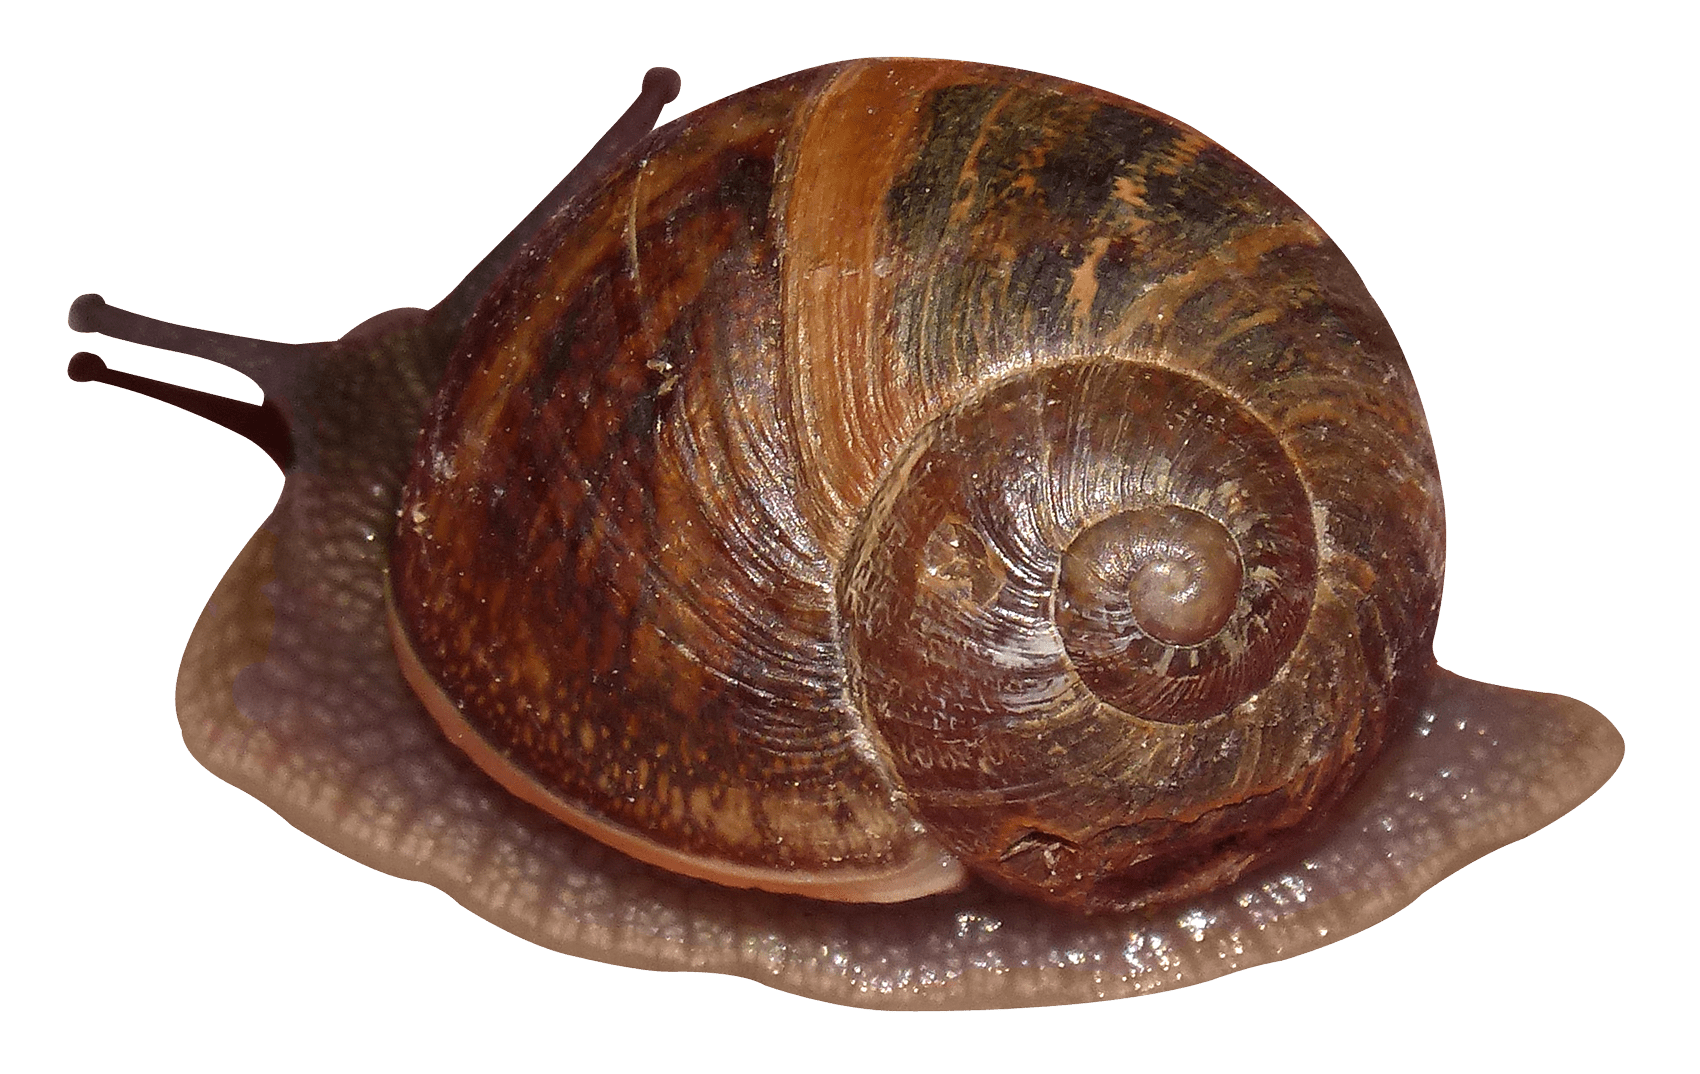
\includegraphics[height=0.25\textwidth]{images/snail.png}

    }
    \caption{Спираль Фибоначчи}
    \label{fig:fibonaccispiral}
\end{figure}

Нарисуйте спираль Фибоначчи, используя класс \code{Arc}, который был создан в~одном из~упражнений.
\end{exercise}

%\include{14/graphics_class_design}
%\include{15/graphing_functions_and_data}
%\include{16/graphical_user_interfaces}
%\include{17/vector_and_free_store}
%\include{18/vectors_and_arrays}
%\include{19/vector_templates_and_exceptions}
%\include{20/containers_and_iterators}
%\include{21/algorithms_and_maps}
%\include{26/testing}


\backmatter
%%=========
% !TEX encoding   = UTF8
% !TEX spellcheck = ru_RU
% !TEX root = ../seminars.tex

%%==================
\chapter{Что дальше}
%%==================
Станете ли вы профессиональным программистом или экспертом по языку \lang{С++}, прочитав эту книгу?\footcite[Текст взят из подраздела 0.1.3]{Stroustrup:2016:ru} Конечно, нет! Настоящее программирование "--- это тонкое, глубокое и очень сложное искусство, требующее знаний и технических навыков. Рассчитывать на то, что за четыре месяца вы станете экспертом по программированию, можно с таким же успехом, как и на то, что за полгода или даже год вы полностью изучите биологию, математику или иностранный язык (например, китайский, английский или датский) или научитесь играть на виолончели. Если подходить к изучению книги серьёзно, то можно ожидать, что вы сможете писать простые полезные программы, читать более сложные программы и получите хорошие теоретическую и практическую основы для дальнейшей работы.

Прослушав этот курс, лучше всего поработать над реальным проектом. Ещё лучше параллельно с работой над реальным проектом приступить к чтению какой~-нибудь книги профессионального уровня (например, \textcite{Stroustrup:2013:en}), более специализированной книги, связанной с вашим проектом, например, документации по библиотеке \name{Qt} для разработки графического пользовательского интерфейса (GUI) или справочника по библиотеке \name{ACE} для параллельного программирования, или учебника, посвященного конкретному аспекту языка \lang{С++}, например \textcite{Koenig:2002:ru, Sutter:2008:ru, Gamma:2004:ru}.

В конечном итоге вам придётся приступить к изучению некоторого другого языка программирования. Невозможно стать профессионалом в области программного обеспечения (даже если программирование не является вашей основной специальностью), зная только один язык программирования.


% !TEX encoding   = UTF8
% !TEX spellcheck = en_US

\clearpage

%\hypersetup{ urlcolor=black }

%\providecommand*{\BibDash}{}
\urlstyle{rm}
\ifdefmacro{\microtypesetup}{\microtypesetup{protrusion=false}}{}
\printbibliography[heading=bibintoc]
\ifdefmacro{\microtypesetup}{\microtypesetup{protrusion=true}}{}
\urlstyle{tt}

%\hypersetup{ urlcolor={urlcolor} }



\appendix
%========
% !TEX encoding   = UTF8
% !TEX spellcheck = ru_RU
% !TEX root = seminars.tex

%%==================
\chapter{Приложение}
%%==================
%%===========================================
\section{Установка и настройка рабочей среды}\label{sect:workEnv}
%%===========================================
{ % hot keys
\newcommand*{\hotkey}[1]{\fbox{\texttt{\small #1}}}
\newcommand*{\hotplus}{{\small\,+\,}}
\newcommand*{\hotkeys}[2]{\hotkey{#1}\hotplus\hotkey{#2}}
\newcommand*{\hotkeyss}[3]{\hotkey{#1}\hotplus\hotkey{#2}\hotplus\hotkey{#3}}



%%============================
\paragraph{ОС \name{Windows}.}
%%============================
Мы настоятельно рекомендуем в качестве \name{IDE} установить \name{Qt\,Creator}. Совместно с ним используйте \name{MinGW-w64} (компилятор, компоновщик, отладчик и прочее).

Удобная \name{UNIX}-подобная командная среда \name{Git\,Bash} идёт в комплекте с системой контроля версий \href{\giturl}{\git}, которая, в свою очередь, входит в состав \name{Smartgit}-а "--- графической облочки над \git-ом. Командная среда, помимо прочего, облегчит тестирование программ в автоматическом и полуавтоматическом режимах. А система контроля версий окажется неотъемлемым элементом разработки сложных программ.

Для установки и настройки компонентов:
\begin{itemfeature}
\item Загрузите \href{\qtcreatorurl}{\name{Qt\,Creator}}\footnote{\nolinkurl{\qtcreatorurl}}, \href{\mingwurl}{\name{MinGW-w64}}\footnote{\nolinkurl{\mingwurl}} и \href{\smartgiturl}{\name{Smartgit}}\footnote{\nolinkurl{\smartgiturl}}.

\item Распакуйте архив \name{MinGW-w64} в каталог \code{c:\backslash{}Program Files} или любой другой каталог, куда вы обычно устанавливаете программы.

И далее, следуя графическим инструкциям из архива
\begin{flushleft}
	\yadisk{cpp-seminars/how-to-s/how-to\_set-up-qt-creator.zip},
\end{flushleft}
выполните последующие пункты.

\item Добавьте путь к компилятору в список стандартных системных путей. Если вы не знаете, как это выполнить

\item Установите \name{Qt\,Creator}, следуя инструкциям установщика.

\item Запустите \name{Qt\,Creator}. Откройте окно настройки параметров из меню \code{Инструменты} \code{->} \code{Параметры}. Во вкладке \code{Комплекты} выберите, скорее всего, единственный комплект \code{Desktop}. В качестве компиляторов для \lang{C} и \lang{C++} выберите из списка \code{MinGW} \GCC{} \code{C} и \code{C++}, соответственно. В качестве отладчика укажите \GDB.

\item Установите \name{Smartgit}, оставляя рекомендуемые (по умолчанию) параметры в тех местах, где вы сомневаетесь, что выбрать.
\end{itemfeature}

Если что-то пошло не так, повторите процедуру \textbf{спокойно}, выполняя \textbf{в точности} все указанные выше действия. Используйте только латиницу для каталогов установки и проектов, иногда русские буквы в путях приводят к ошибкам в \name{Qt\,Creator}-е.

И теперь не получилось? Хм-м... Тогда обратитесь за помощью к студентам старших курсов или преподавателю.



%%=========================
\paragraph{ОС \name{UNIX}.}
%%=========================
Пользователи \name{UNIX} и подобных ей операционных систем могут установить при помощи системы управления пакетами (например, \code{apt} в \name{Ubuntu}) дистрибутив \name{Qt\,Creator} совместно со средствами сборки \name{GNU} \GCC{} или \code{Clang}, а также систему контроля версий \git{} и \name{Smartgit}.



%%=============================
\section{Редактирование текста}\label{sect:typing}
%%=============================
Набор исходного текста "--- неотъемлемая часть разработки программ. Используйте <<горячие>> клавиши для более быстрого редактирования. Краткий список наиболее популярных комбинаций, поддерживаемых даже простыми редакторами:

\begin{longtable}[l]{@{}rp{0.7\textwidth}@{}}
\endhead
\endfoot

\hotkeys{Ctrl}{A}  & Выделить всё.\\[0.5em]

\hotkeys{Ctrl}{C}  & Скопировать выделение. \\
\hotkeys{Ctrl}{V}  & Вставить. \\[0.5em]

\hotkeys{Ctrl}{Z}  & Отменить последнее действие. \\[0.5em]

\hotkey{Home} & Переместить курсор в начало\slash{}конец текущей строки. \\
\hotkey{End}  & \\[0.5em]

\hotkeys{Shift}{Home} & Выделить символы с текущей позиции и до начала\slash{}конца строки. \\
\hotkeys{Shift}{End}  & \\[0.5em]

\hotkeys{Ctrl}{Home} & Переместить курсор в начало\slash{}конец файла. \\
\hotkeys{Ctrl}{End}  & \\[0.5em]

\hotkeys{Ctrl}{\leftarrow}  & Переместить курсор по словам. \\
\hotkeys{Ctrl}{\rightarrow} & \\
\end{longtable}

\noindent Дополнительные полезные комбинации в \name{Qt\,Creator}:
\begin{longtable}[l]{@{}rp{0.7\textwidth}@{}}
\endhead
\endfoot

\hotkeys{Ctrl}{I} & Выровнять отступ (\textenglish{\textbf{i}ndent}) текущей строки или выделения. \\[0.5em]

\hotkeys{Ctrl}{\slash} & Комментировать\slash{}раскомментировать текущую строку или выделение. \\[0.5em]

\hotkeyss{Ctrl}{Shift}{R} & Переименовать имя под курсором. \\[0.5em]

\hotkeyss{Ctrl}{Shift}{\uparrow}   & Сместить текущую строку вверх\slash{}вниз. \\
\hotkeyss{Ctrl}{Shift}{\downarrow} & \\[0.5em]

\hotkeyss{Alt}{Shift}{\uparrow}   & Редактировать столбец. \\
\hotkeyss{Alt}{Shift}{\downarrow} & \\
\end{longtable}

Полезно научиться набирать текст вслепую, то есть не глядя на клавиатуру. В сочетании с использованием горячих клавиш это позволяет достичь существенного ускорения при работе с исходным кодом. Таким образом, остаётся больше времени для размышлений над структурой и логикой самой программы. В качестве примера он-лайн клавиатурного тренажёра приведём \href{\typingtutorurl}{эту}\footnote{\nolinkurl{\typingtutorurl}} ссылку.

} % hot keys



%%====================
\section{Unix утилиты}\label{sect:utils}
%%====================
Совместно с командной средой (\name{bash} "--- \textenglish{\textbf{b}ourne \textbf{a}gain \textbf{sh}ell}) поставляется широкий набор полезных программ, или утилит (\textenglish{utilities}).

\console/$ cd dir/%$

\textenglish{\textbf{c}hange \textbf{d}irectory} "--- перейти в каталог \code{dir}. Если каталог опущен, то перейти в домашний каталог. (Определяется значением переменной среды \code{HOME}.) Файловая система \textenglish{Unix} представляет собой единое дерево, и любой абсолютный путь начинается с корня (\code{/}). Точка (\code{.}) означает текущий каталог, две точки (\code{..}) "--- родительский каталог.

\console/$ cd ../%$

Перейти в родительский каталог.

\console|$ cd /|%$

Перейти в корневой каталог.

\console/$ pwd/%$

\textenglish{\textbf{p}rint \textbf{w}orking \textbf{d}irectory} "--- вывести на экран абсолютный путь к текущему каталогу.

\console/$ ls dir/%$

\textenglish{\textbf{l}i\textbf{s}t} "--- вывести на экран содержимое каталога \code{dir}. Если каталог опущен, то по умолчанию используется текущий каталог.

\console/$ man cmd/%$

\textenglish{\textbf{man}ual} "--- вывести на экран подробную справку о команде \code{cmd}.

\console/$ cmd --help/%$

Вывести на экран короткую справку о команде \code{cmd}. Полезно, если утилита \code{man} недоступна.

\console/$ mkdir dir/%$

\textenglish{\textbf{m}a\textbf{k}e \textbf{dir}ectory} "--- создать каталог \code{dir}.

\console/$ rmdir dir/%$

\textenglish{\textbf{r}e\textbf{m}ove \textbf{dir}ectory} "--- удалить пустой каталог \code{dir}.

\console/$ rm file/%$

\textenglish{\textbf{r}e\textbf{m}ove} "--- удалить файл. Используя опцию \code{-r} можно рекурсивно удалить непустой каталог.

\console/$ mv src dst/%$

\textenglish{\textbf{m}o\textbf{v}e} "--- перемещает/переименовывает файл \code{src} в \code{dst}. Имя \code{dst} может быть каталогом, тогда \code{mv} перемещает \code{src} туда.

\console/$ cat file.../%$

\textenglish{\textbf{cat}enate} "--- связывает файлы и выводит объединённое содержимое на экран.

\console/$ less file/%$

Более мощный аналог утилиты \code{more} "--- постраничного фильтра для просмотра файлов. Часто применяется для буферизации вывода на экран, используя конвейер:

\console/$ odjdump -d prog | less/%$


\console/$ vim file/%$

\textenglish{\textbf{v}isual editor \textbf{im}proved} "--- открыть файл для редактирования. Пройти вводный курс по использованию этого мощного редактора можно запустив команду:

\console/$ vimtutor/%$



%%==================================
\section{Интерпретатор \name{shell}}\label{sect:shell}
%%==================================
Когда система (в терминале) выдаёт приглашение \code{\$} и вы вводите команды для выполнения, вы имеете дело не с ядром самой системы, а с неким посредником, называемым интерпретатором команд, или \name{shell}\footnote{Более подробно об интерпретаторе \name{shell} и других возможностях системы \textenglish{Unix} излагается, например, в книге \fullcite{Kernighan:1992:ru}}. Это обычная программа, но она может делать удивительные вещи. Применение программы--посредника обеспечивает три главных преимущества:

\begin{itemfeature}[itemsep=\baselineskip]
  \item Сокращённые имена файлов: можно задать целое множество файлов в качестве аргументов команде, указав шаблон для имён: \name{shell} будет искать файлы, имена которых соответствуют заданному шаблону.

  \console/$ ls *.cpp *.c/%$

  Вывести на печать имена всех файлов в текущем каталоге, которые оканчиваются на~\code{.cpp} или \code{.c}. Символ \code{*} в шаблоне соответствует любой последовательности символов. Поддерживаются и другие специальные символы для задания шаблона.


  \item Переключение ввода--вывода: вывод любой программы можно направить в файл, а не на терминал, ввод можно получать из файла, а не с терминала. Ввод и вывод можно даже передать другим программам.

  \console/$ ls *.cpp > cppfiles.txt/%$

  Имена всех файлов, оканчивающихся на~\code{.cpp}, направить в файл \code{cppfiles.txt}. Файл будет создан, если не существует, или перезаписан, если существует.

  \console/$ wc -l < main.cpp/%$

  Подсчитать количество строк (опция \code{-l}) в файле \code{main.cpp}.

  \console/$ cat main.cpp | wc -l/%$

  То же. Символ~\code{|} обозначает конвейер. Вывод команды слева передаётся на ввод команде справа. Можно организовывать в конвейере цепочку любой длины.

  \console/$ wc -l main.cpp/%$

  То же, используя лишь возможности самой утилиты \code{wc} (\textenglish{\textbf{w}ord \textbf{c}ount}).


  \item Создание собственной среды: можно определить свои собственные команды и правила сокращений.
\end{itemfeature}



%%==========================================
\section{Рисование графиков в \lang{Python}}\label{sect:pyplot}
%%==========================================
Каждый язык имеет свои достоинства и недостатки и, как правило, нацелен на эффективное решение определённого класса задач. Совместное использование разных языков часто помогает сократить усилия при разработке программ и повысить гибкость либо удобство создаваемых инструментов. Попробуем продемонстрировать это на примере визуализации результатов обработки данных лабораторной работы по физике, которые можно получить методом наименьших квадратов, рассмотренным в разделе~\ref{chap:helloworld} (также см. упр.~\ref{ex:plot} на странице~\pageref{ex:plot}).

\begin{figure}[ht]
  {\centering
    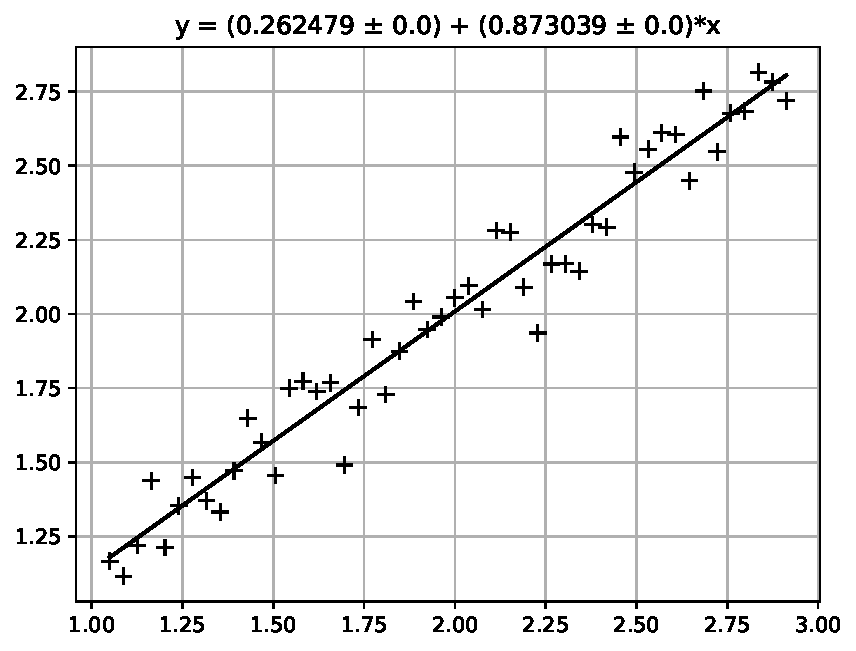
\includegraphics[width=0.6\textwidth]{images/line_approx.pdf}

  }
  \caption{Визуализация при помощи \name{Matplotlib}}
  \label{fig:pyplot}
\end{figure}

В языке \lang{C++} нет встроенных графических средств. Для этого необходимо использовать сторонние библиотеки. Работа с подобными инструментами не всегда настолько проста, как хотелось бы. А настройка внешнего вида координатных осей, изображаемых кривых и точек может потребовать перекомпиляции всей программы.

Одним из действительно удобных для этого случая решений является написание сценария (\textenglish{script}) на интерпретируемом языке. \href{\pythonurl}{\lang{Python}} относится к этому ряду языков и имеет мощную поддержку разнообразных средств практически прямо <<из коробки>>. Ниже приведён вариант решения нашей задачи с использованием пакета \href{\matplotliburl}{\name{Matplotlib}}.

\begin{center}
  \yadisk{cpp-seminars/examples/01/plot.py}
\end{center}

\inputminted[linenos, fontsize=\small]{py}{01/src/plot.py}

Совместить использование разработанных нами отдельных инструментов можно при помощи командной среды. Для этого достаточно всего одной строки (см. страницу~\pageref{sect:shell}):
\begin{consolecode}
$ ./lsm line_approx.txt | xargs python3 plot.py
\end{consolecode}

\noindent Результат в виде графического файла \code{line\_approx.pdf}, изображён на рисунке~\ref{fig:pyplot}.


\end{document}
